\documentclass[a4paper,11pt,uplatex]{jsarticle}

\usepackage[dvipdfmx]{graphicx,xcolor}% ドライバ指定
\usepackage[top=30truemm,bottom=30truemm,left=25truemm,right=25truemm]{geometry} % 余白設定

% 画像
\usepackage{here, subfig}
\usepackage{docmute} % ファイル分割用
\usepackage[cc]{titlepic}

% 数式関連
\usepackage{amsmath,amsfonts,amssymb,mathtools,amsthm}
\usepackage{bm} % ボールド体のベクトルを出力するときには\vb{a}ではなく\bm{a}としてください。\bmの方が綺麗に出力できる。
\usepackage{empheq} % 連立方程式をきれいに書いてくれる
\usepackage{physics} % 微分記号とか
\usepackage[separate-uncertainty]{siunitx} % SIUNITX

% 数式、図、表番号の変更
\makeatletter
\@addtoreset{equation}{section} % 章ごとに番号をリセット
\@addtoreset{figure}{section}
\@addtoreset{table}{section}
\def\theequation{\thesection.\arabic{equation}} % 章.何番目 と変更
\def\thefigure{\thesection.\arabic{figure}}
\def\thetable{\thesection.\arabic{table}}
\makeatother

% -------------------
% 定理環境付近
\usepackage{tcolorbox} % 色付きの囲み
\tcbuselibrary{breakable, skins, theorems}
\usepackage{ascmac} % 囲み \begin{itembox}ができる。

% ----------

\usepackage{enumitem} % enumium環境いじるために必要
\renewcommand{\labelenumi}{\theenumi.}
\renewcommand{\theenumi}{\Alph{enumi}}

% ------------ url関係
\usepackage{url}
\usepackage[dvipdfmx]{hyperref}
\hypersetup{
	 colorlinks=true,
	 citecolor=blue,
	 linkcolor=black,
	 urlcolor=blue
}
\usepackage{pxjahyper}
% ---------

% 表関連のパッケージ
\usepackage{booktabs}
\usepackage{multirow}
\usepackage{longtable}
\usepackage{arydshln}% 表で破線を使うため
\usepackage{multicol}
% longtableをusepackageする場合は順番が重要らしいです。longtableとarydshlnの順番逆にしたらエラーはく(コンパイルはできるが…)

\renewcommand{\labelitemii}{・}

\usepackage[greek, japanese]{babel}
\usepackage{teubner}	% 古代(古典)ギリシア語表記指定



% 大槻使用
\usepackage{color}
\newcommand{\red}[1]{\textcolor{red}{#1}}
\newcommand{\blue}[1]{\textcolor{blue}{#1}}
\usepackage{ulem}

% 能崎使用
%背景
\usepackage{wallpaper}
\title{CREATE2 成果報告書}
\date{\today}
\author{松本侑真\thanks{C-59J PM}\and{大槻渉}\thanks{構造系責任者}
\and{能崎直紀}\thanks{電装系責任者}\and{佐野泰笙}\thanks{シミュレーション系責任者}
\and{川北魁人}\thanks{推進系責任者}}

\begin{document}
\maketitle


\begin{abstract}
	第21回伊豆大島共同打上実験におけるCREATE2の打上結果について、本成果報告書で詳細に述べる。本打上実験では団体初の動翼機構を搭載したC-59Jを打ち上げ、ロール制御ミッションに挑戦した。
	\footnote{以下ではCERATE2のプロジェクトを指す場合でも、打上機体名である「C-59J」と呼称する。}
	打上結果としては、パラシュート解放による減速落下に成功し、各基板のセンサによるデータを回収することができた。
	データ解析によると、制御開始直後から機体のロール角度が目標ロール角度に速やかに収束し、その後の追従精度も十分なものであった。
	そのためC-59Jのメインミッションである、ロール制御技術を確立させ、ロール制御を成功させるという目標は達成することができた。
	しかし、本打上実験において新たな課題も見つかった。本報告書では、プロジェクト概要、C-59Jの打上結果とデータ解析、プロジェクトを通して見つかった課題について記す。
\end{abstract}
\newpage
\tableofcontents
\newpage

\section{プロジェクト概要}
本プロジェクトでは、団体初の動翼機構をC-59Jに搭載し、エンジン燃焼終了後からパラシュート開傘までのロール制御を行った。
本プロジェクトの目的は、ロケットのロール制御技術を獲得・実証し、姿勢制御技術の足掛かりを得ることである。
ロール制御については、対気速度によって変化するロールモーメントの大きさを考慮しながら、ロール角度を一定に保つようにフィードバック制御を行う。
なお、機体に搭載したピトー管により、飛行時の対気速度をリアルタイムで取得した。

\subsection{ミッション目標}
本プロジェクトのミッション目標は以下の通りである
\begin{itemize}
	\item ピトー管によって対気速度をリアルタイムで取得する。
	\item 燃焼終了からパラシュート開傘までのロール制御を行う。
\end{itemize}

1番のミッション目標は機体のロール制御を行うことである。ところで、ロール制御の精度を上げるためには対気速度をリアルタイムで取得する必要があり、
その方法の1つとしてピトー管を搭載することが挙げられる。
しかし、現在のCREATEにはピトー管の作成・評価技術が存在していないため、第18回能代宇宙イベント\footnote{2022年8月11日から2022年8月19日まで行われた、秋田県能代市を会場とした宇宙イベントである。\\
	能代宇宙イベント公式ホームページ:\url{http://www.noshiro-space-event.org/}}
においてC-61J\footnote{第21回伊豆大島共同打上実験にてCREATEが打ち上げた2021年度新入生機体である。}がC-59Jに先行してピトー管を搭載し、技術検証をする予定であった。
しかし、C-59Jと同じ第21回伊豆大島共同打上実験での打上げとなったため、ピトー管の技術検証もC-59Jのミッション目標に含まれることになった。なお、サクセスクライテリアについてはロール制御ミッションのみに設定してある。

\subsection{ミッション背景}
次に、ミッション背景について述べる。CREATEのロケットはロール運動しながら飛行していることが以前の打上実験から判明している。
本来ならばロール運動をしないような構造設計をしているため、ロール運動をしながら飛行することは好ましくない。
特に二段式技術実証機であるC-43Jプロジェクトにおいて、機体の姿勢角条件が二段目分離条件を満たしておらず、電装部の安全機構により二段目が放出されなかった。
以上の結果より、機体の姿勢制御技術を発展させ、より安定した飛行を目指すことが団体の課題であった。

また、ピッチ・ヨー制御と比較してロール制御を行うメリットとして、制御による飛行経路の影響が少ないということが挙げられる。
これは、ロール回転運動がピッチ・ヨー回転運動に影響を与えないことに基づいている。
機体が予想外のピッチ・ヨー回転運動をする場合、機体の飛行経路に大きな影響を与えることが知られている。
すなわち、ピッチ・ヨー制御を行うことはロール制御よりも安全面から困難であると考えた。
そのため、C-59Jでは姿勢制御技術の発展の第一歩としてロール制御をミッションとした。

\newpage
\subsection{サクセスクライテリアについて}
以下の表\ref{tab:success_criteria}に本プロジェクトのサクセスクライテリアを示す。なお、FULLのサクセスクライテリアについては表とは別に詳述する。
\begin{table}[H]
	\centering
	\caption{サクセスクライテリア}
	\begin{tabular}{cp{60mm}p{60mm}} \toprule
		     & \multicolumn{1}{c}{内容}                               & \multicolumn{1}{c}{判定条件}             \\ \midrule
		MIN  & 地上で制御プログラムを実行し、動翼の適切な動作を確認する。                        & 動画とデータ解析により、意図した動翼の動作が実現していることを確認する。 \\ \midrule
		FULL & ロール制御を成功させる。                                         & 搭載カメラの映像とデータ解析によって確認する。              \\ \midrule
		ADV  & 制御前に機体がロールをしていた場合、制御中は目標角からのロール角度を\SI{90}{deg}以下にする。 & データ解析で内容を達成しているか確認する。                \\
		\bottomrule
	\end{tabular}
	\label{tab:success_criteria}
\end{table}
\subsubsection*{FULLのサクセスクライテリアについて}
FULLのサクセスクライテリアの意味としてのロール制御の成功条件を述べる。まずは以下に3つの文を示す:
\begin{enumerate}
	\item ある程度一定方向を向き続けた映像が撮れている。
	\item 6軸センサのデータから機体のロール角度が一定に保たれていることがわかる。
	\item 意図したロール制御が実現されている。
\end{enumerate}

FULLのサクセスクライテリアでの意味としてロール制御が成功しているとは、文Aと文Bが同時に満たされている場合であると定義する。
次に、3つの文をサクセスクライテリアの成功可否に用いる理由について述べる。
そもそもロール制御が成功しているとは、「ロール制御が何らかの結果として成功しており、実際にロール角度が一定に保たれていること」と、「ロール制御が制御系の正常な動作によって引き起こされたものであること」を同時に満たしている状況のことである。
ここで文Aと文Bは、ロール角度が一定に保たれていることを確認するために導入した。
すなわち、C-59Jの機体動翼部に搭載しているカメラ映像や6軸センサでのロール角の値を用いることで、制御部に依らずにロール角度が一定に保たれていることを確認できる条件とした。
そして文Cは、ロール角度が一定に保たれているかとは独立に、制御系の正常な動作を定量的に確認するために導入した。

文Aの達成可否については機体に搭載したカメラによって判定する。ロール制御が成功している場合には、カメラ映像でロール角度が一定に保たれていることが目視で判別することができる。
文Bの達成可否については6軸センサの各速度データを積分した結果から判定する。
最後に、文Cの達成可否については電装データによって定量的に判定する。先に述べたように、カメラ映像によってロール制御が成功していると判断できても、制御系が正常に機能していることの確認にはならない。
すなわち、カメラの映像で定性的にロール制御の成功を確認するだけでなく、それが意図した制御によって実現されたことを確認する必要がある。
したがって、ロール角度や動翼角度のログデータ、実際の制御系の応答、目標角度の追従精度などから定量的に成功可否を判断する。

\newpage
\subsection{機体ロゴ}
C-59J(愛称:IRIS)の機体ロゴを以下の図\ref{fig:sum_kitairogo}に示す。
\begin{figure}[H]
	\centering
	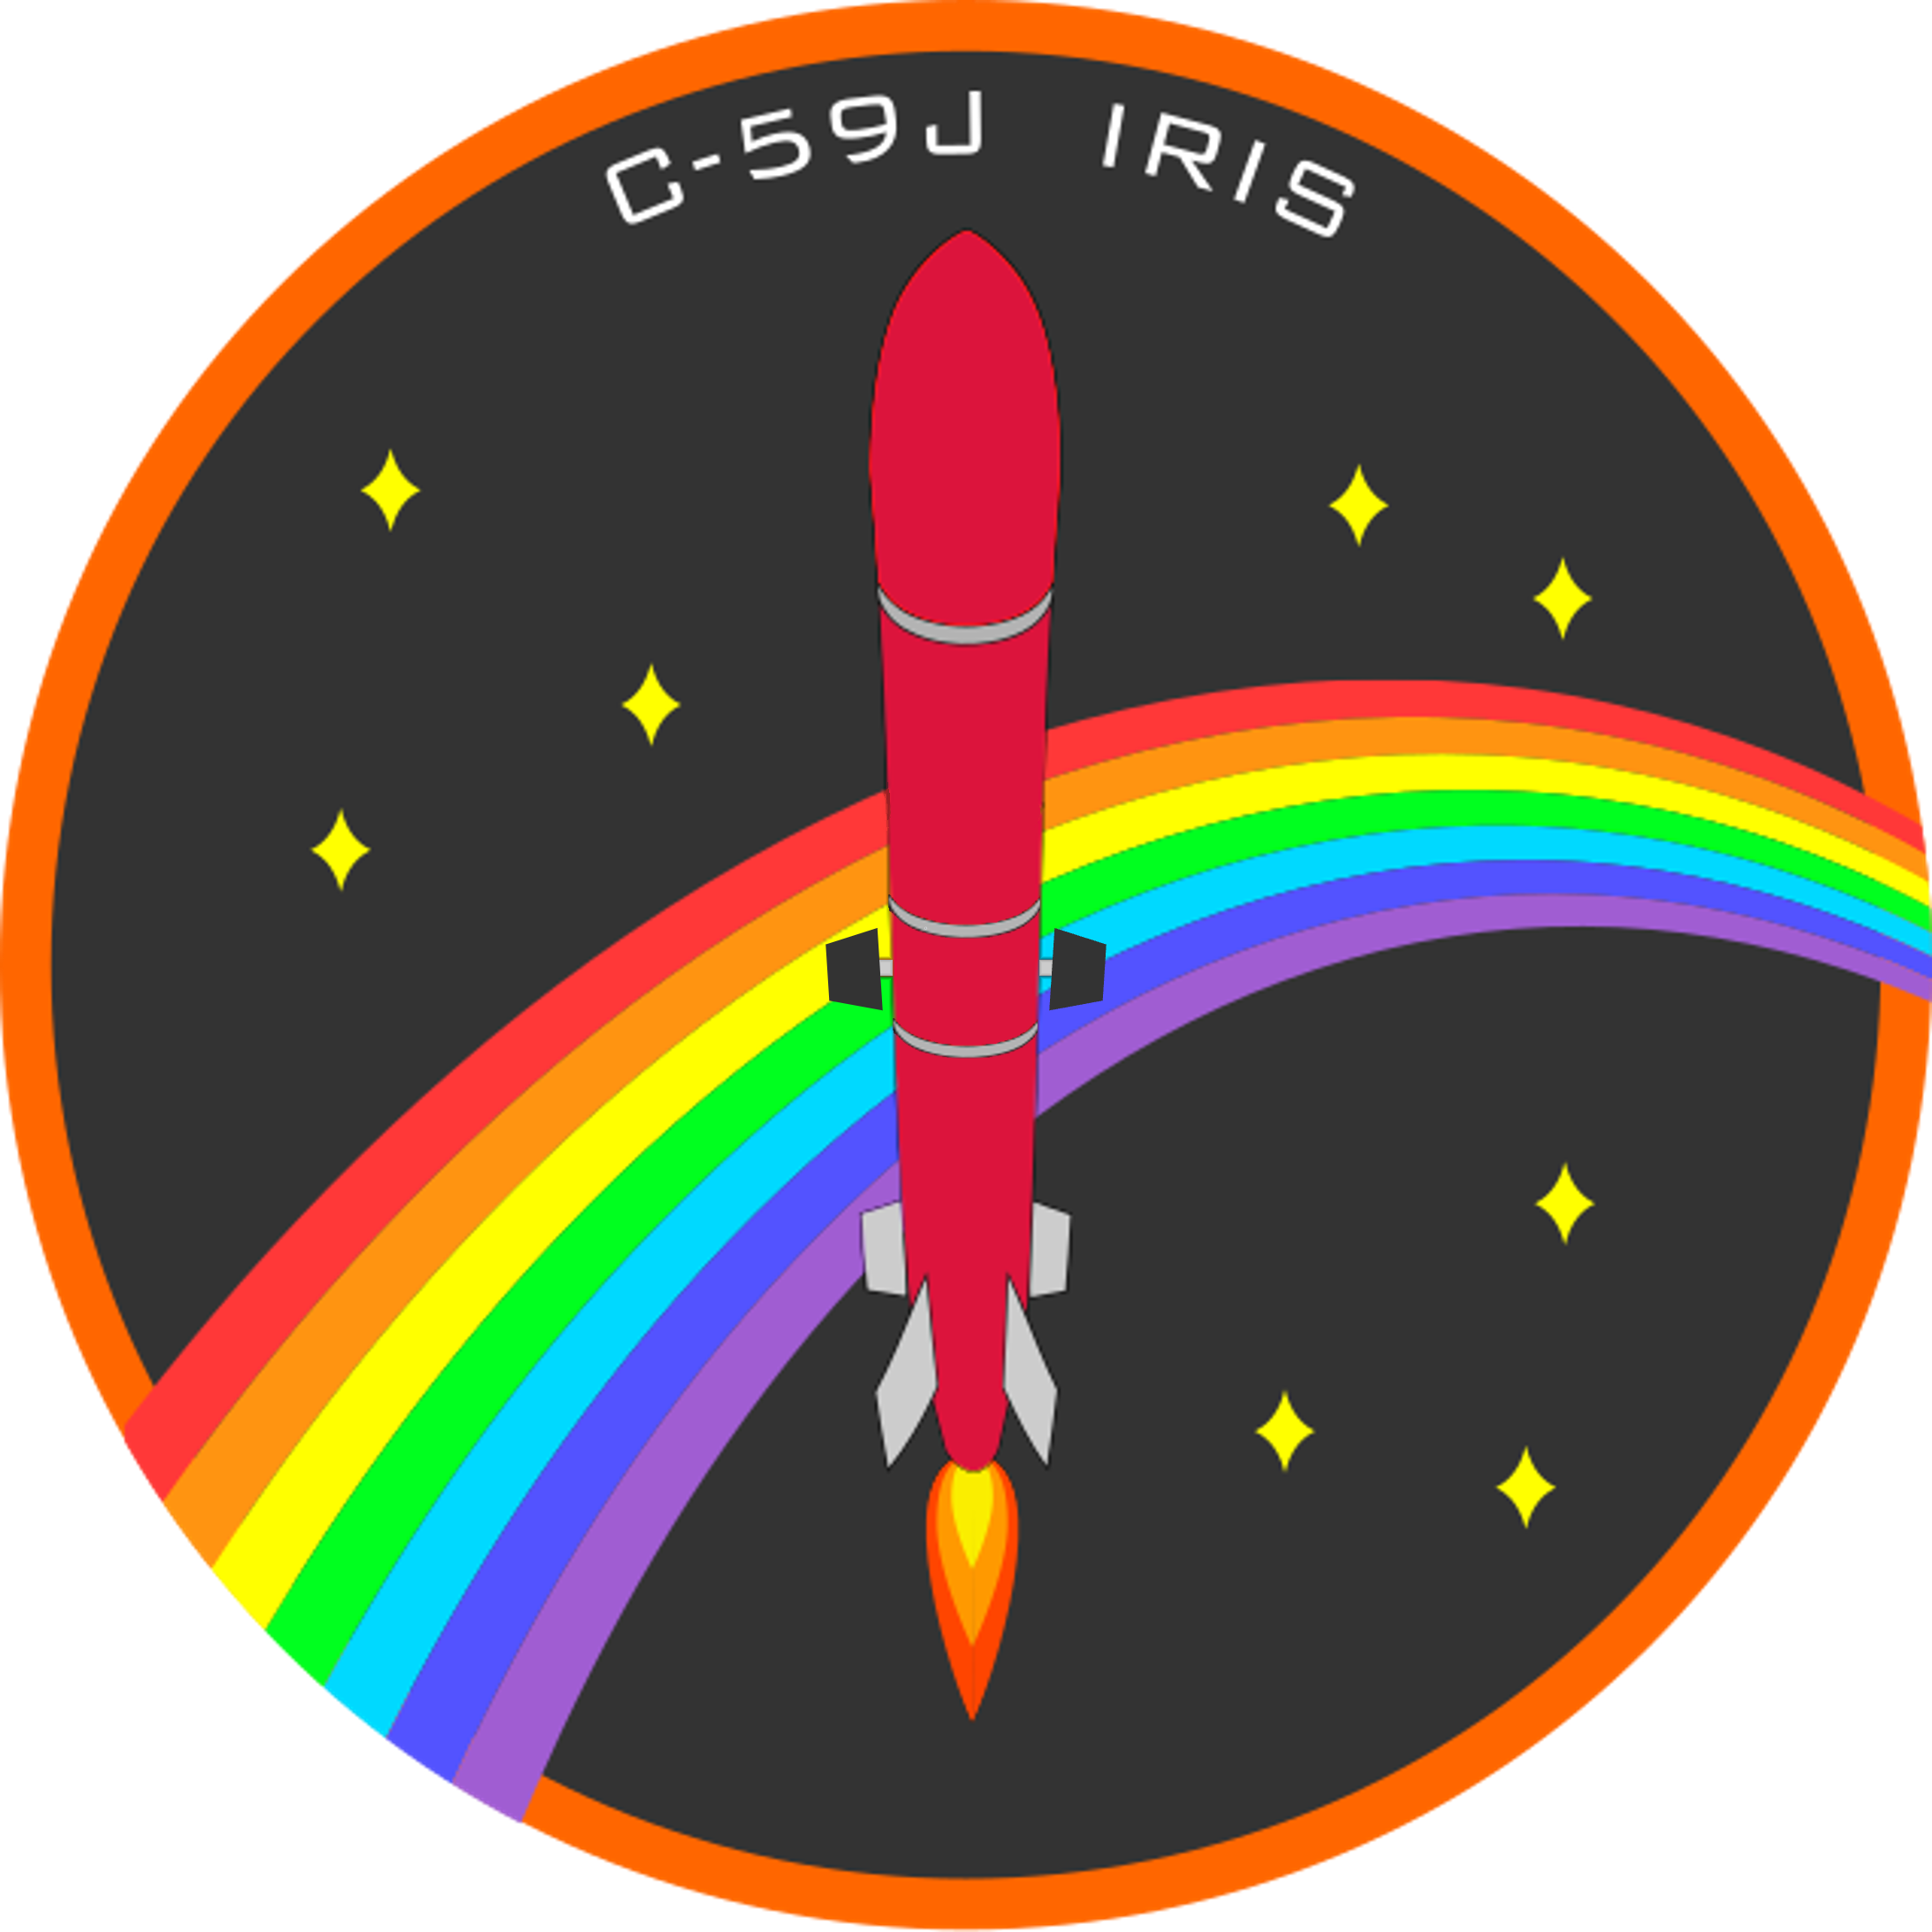
\includegraphics[width=0.5\linewidth]{pic_summary/newlogo.png}
	\caption{機体ロゴ}
	\label{fig:sum_kitairogo}
\end{figure}
ロゴデザインのモチーフは、C-59Jの愛称である``IRIS''からきている。
IRISはギリシャ神話に登場する虹の女神IRIS (\foreignlanguage{greek}{{>~I}ris})から取られており、機体に虹が架かる様子を表している。

\newpage
\section{構造系開発概要}
\subsection{機体概要}
機体諸元を表\ref{s_59syogen}に示す。
また、機体外観図、各部材位置、各部品詳細をそれぞれ図\ref{s_gaikei}、図\ref{s_iti}、表\ref{s_buhin}に示す。
また、実機写真を図\ref{s_real1}、図\ref{s_real2}に示す。

\begin{table}[H]
	\centering
	\caption{機体諸元}
	\begin{tabular}{ccl} \toprule
		名称     & 諸元            & 備考     \\\midrule
		機体名称   & IRIS(C-59J)            \\
		全長     & \SI{1541}{mm} & ピトー管あり \\
		       & \SI{1486}{mm} & ピトー管なし \\
		直径     & \SI{91}{mm}            \\
		乾燥質量   & \SI{5944}{g}           \\
		重心位置   & \SI{707}{mm}  & 機体後端より \\
		圧力中心位置 & \SI{523}{mm}  & 機体後端より \\
		静安定静余裕 & 11.6          & 最小値    \\
		       & 12.8          & 最大値    \\
		\bottomrule
	\end{tabular}
	\label{s_59syogen}
\end{table}

\begin{figure}[H]
	\centering
	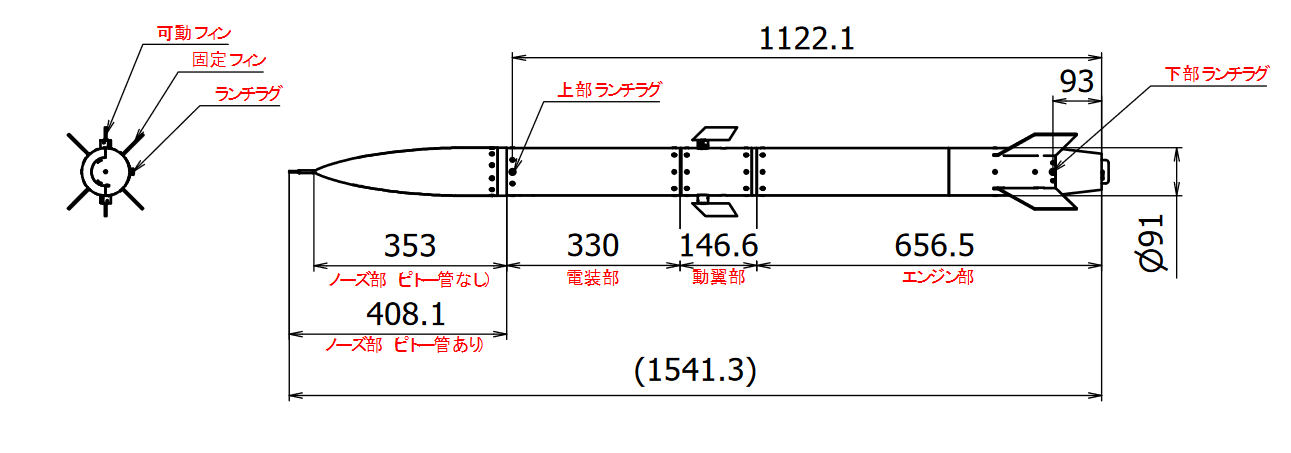
\includegraphics[width=1.1\linewidth]{pic_str/s_sunpou.png}
	\caption{機体外観図}
	\label{s_gaikei}
\end{figure}

\begin{figure}[H]
	\centering
	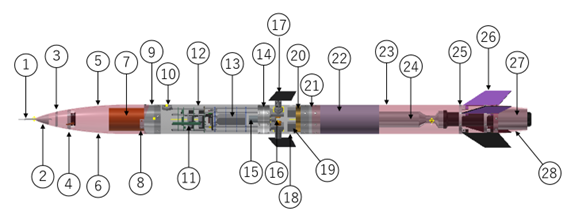
\includegraphics{pic_str/s_iti.png}
	\caption{各部材位置}
	\label{s_iti}
\end{figure}

\renewcommand{\arraystretch}{0.9}
\begin{longtable}[H]{cclll}
	\caption{各部品詳細図}
	\label{s_buhin}                                                    \\
	\toprule
	区画    & No. & 部品名       & 材質    & 型番及び説明                           \\ \hline \endhead
	ノーズ部  & 1   & ピトー管      & A5052 & 内製                               \\
	      & 2   & ノーズトップ    & ABS   & ピトー管固定用                          \\
	      & 3   & ピトー管用基板   & N/A   & 電装概要に記載                          \\
	      & 4   & 減速機構      & N/A   & 従来機体から踏襲                         \\
	      & 5   & ノーズコーン    & CFRP  &                                  \\
	      & 6   & フェアリング    & CFRP  & 開放部                              \\
	      & 7   & パラシュート    & ナイロン  &                                  \\
	      & 8   & リカバリーネイル  & ABS   & フェアリング抑え                         \\\midrule
	      & 9   & NAカプラー    & A5052 &                                  \\ \midrule
	電装部   & 10  & 電源投入スイッチ  & ABS   & \ref{switch}節に記載                 \\
	      & 11  & 電装タワー     & N/A   &                                  \\
	      & 12  & 電装チューブ    & GFRP  &                                  \\
	      & 13  & LiFeバッテリー & N/A   & ROBOパワーセル F3-1450タイプ(Li-Fe)      \\ \midrule
	      & 14  & ARカプラー    & A5052 &                                  \\ \midrule
	動翼部   & 15  & 動翼制御用モータ  & N/A   & Maxon(製品番号:134164、110160、201937) \\
	      & 16  & 動翼機構      & N/A   & \ref{douyoku}節に記載                \\
	      & 17  & 可動フィン     & アクリル  &                                  \\
	      & 18  & 動翼チューブ    & CFRP                                     \\
	      & 19  & カメラ       & N/A   & MD25                             \\
	      & 20  & 錘         & 真鍮    &                                  \\\midrule
	      & 21  & REカプラー    & A5052 &                                  \\ \midrule
	エンジン部 & 22  & スタイロフォーム  & N/A   & エンジン抑え                           \\
	      & 23  & エンジンチューブ  & CFRP                                     \\
	      & 24  & エンジン      & N/A   & HyperTEK J250                    \\
	      & 25  & フィンブロック   & ABS   & 固定フィン固定用                         \\
	      & 26  & 固定フィン     & アクリル  &                                  \\
	      & 27  & エンジン受け    & A5052 & 2部品で構成                           \\
	      & 28  & テールコーン    & ABS   & \ref{tale}節に記載                   \\
	\bottomrule
\end{longtable}
\renewcommand{\arraystretch}{1.0}


\begin{figure}[H]
	\centering
	\includegraphics[scale = 0.1]{pic_str/s_59_real_pic.jpg}
	\caption{実機写真}
	\label{s_real1}
\end{figure}

\begin{figure}[H]
	\centering
	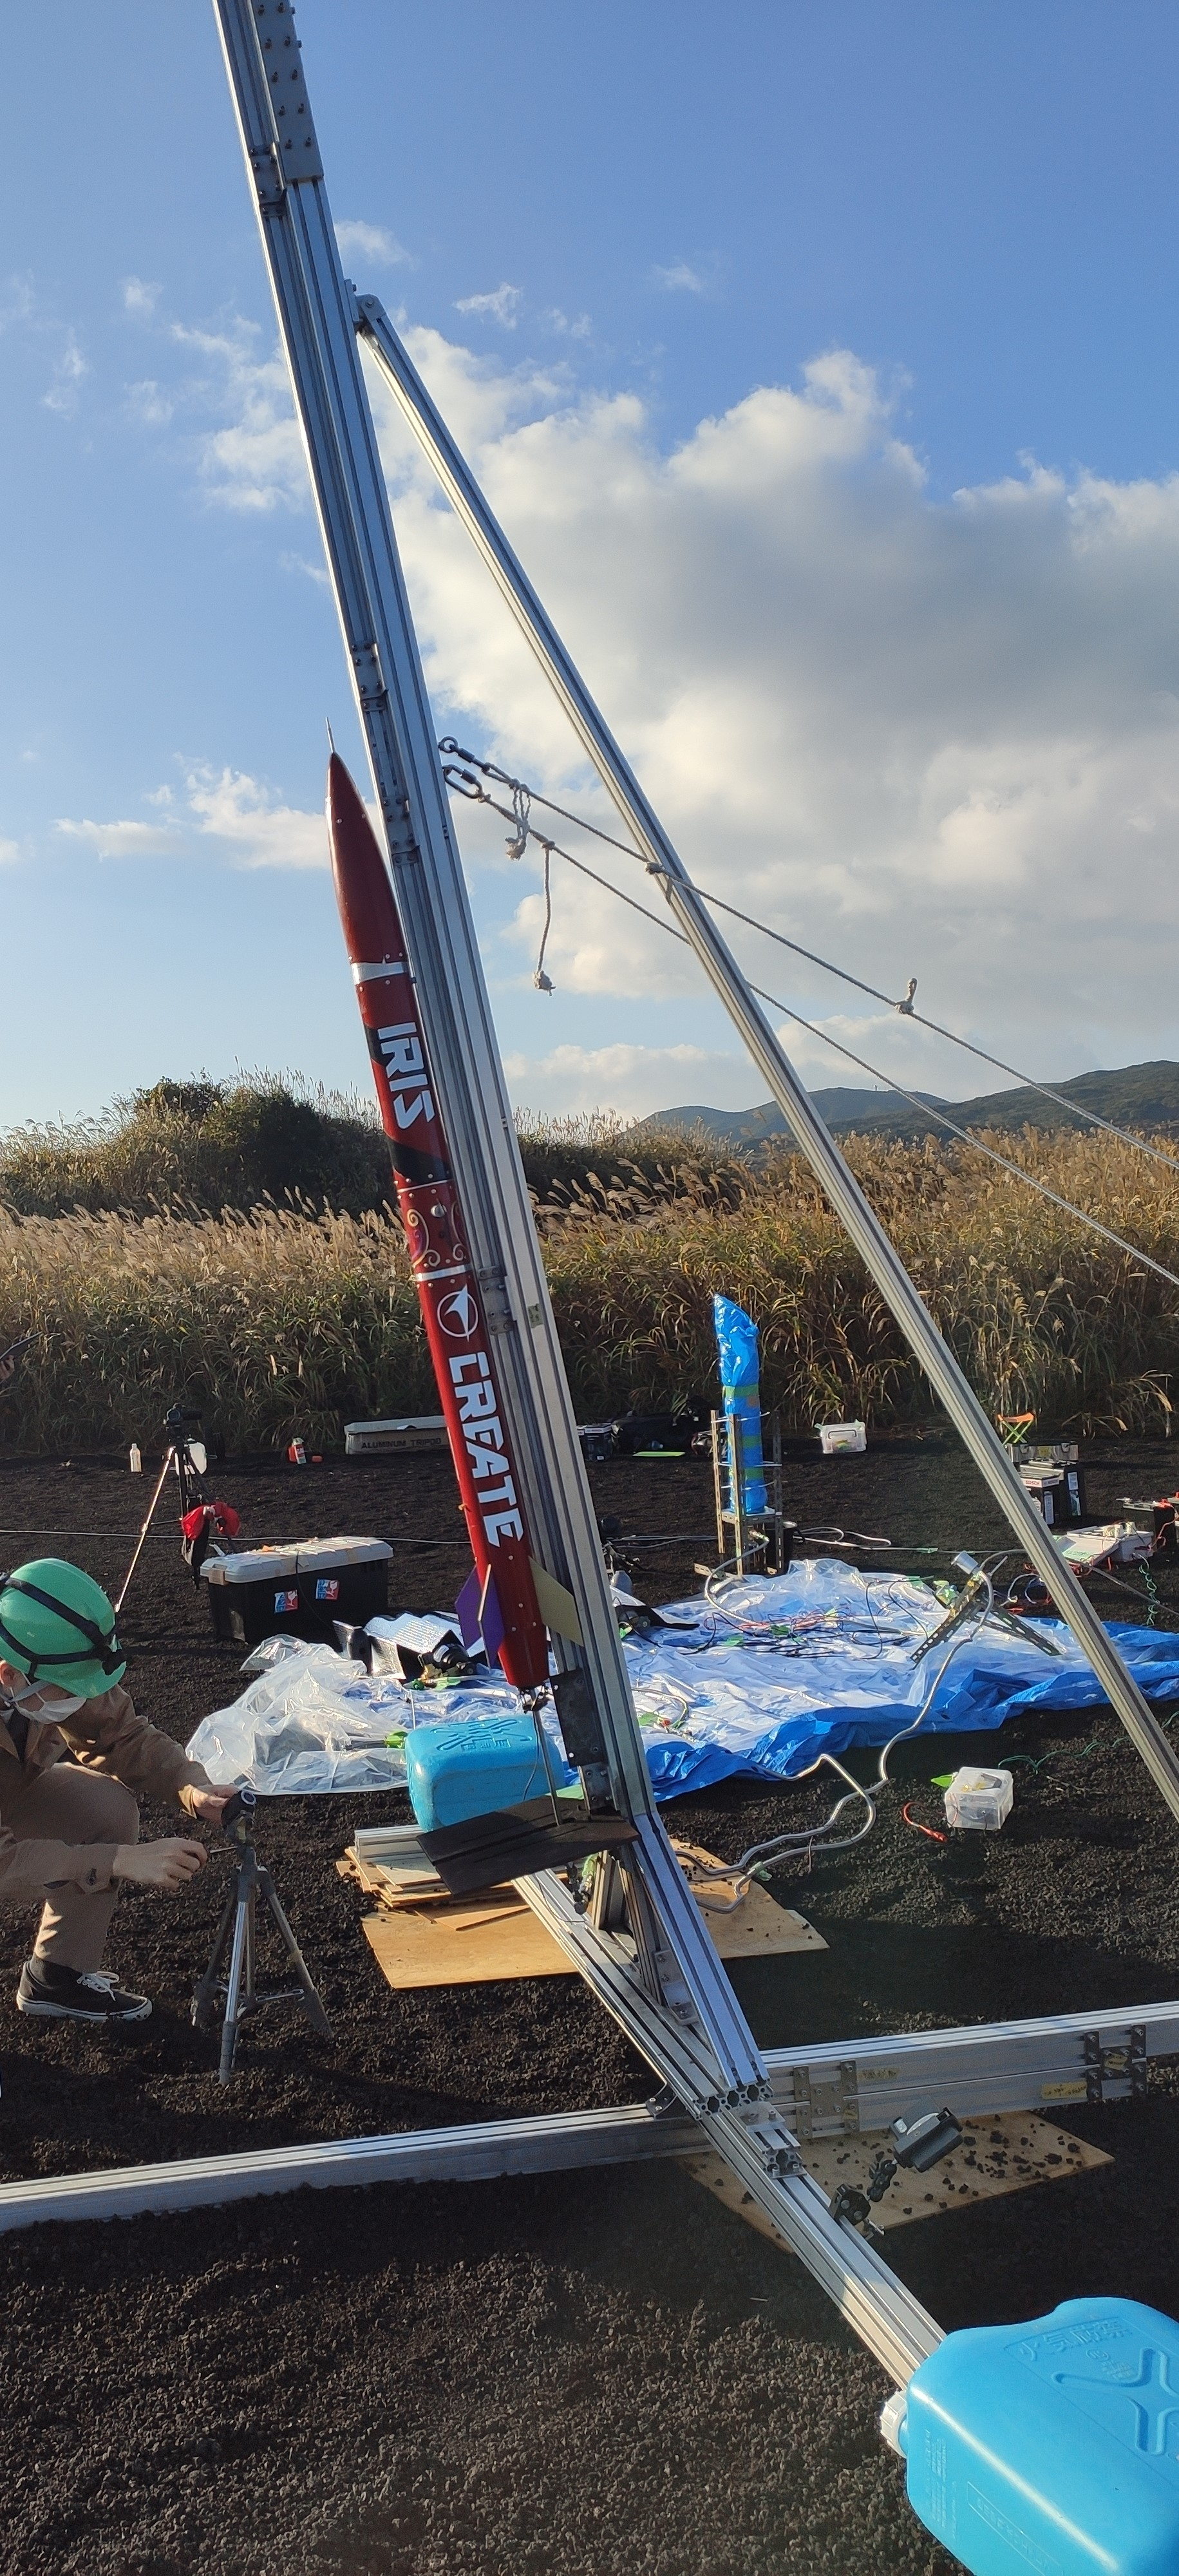
\includegraphics[scale = 0.1]{pic_str/s_59_launcher.jpg}
	\caption{実機写真(ランチャー挿入)}
	\label{s_real2}
\end{figure}

本機はロール制御ミッション達成のため、新たに可動フィンを設置していることが特徴である。
図\ref{s_gaikei}左側記載の側面図に示すように、固定フィン4枚、可動フィン2枚を搭載している。
フィンの位相角は、ランチラグを\SI{0}{deg}としたとき、固定用フィンは\SI{45}{deg}、\SI{135}{deg}、\SI{225}{deg}、\SI{315}{deg}であり、可動フィンは\SI{90}{deg}、\SI{270}{deg}となっている。
これは、可動フィンによって発生した乱流が後方の固定フィンに影響を与えないようにするためである。

\subsection{動翼機構}
\label{douyoku}
本節では、ロール制御ミッションのために新たに追加した動翼部について記す。
動翼機構のCAD図と写真、外形の様子をそれぞれ図\ref{s_r_all}、図\ref{s_r_pic}、図\ref{s_r_outer}に示す。

\begin{figure}[H]
	\centering
	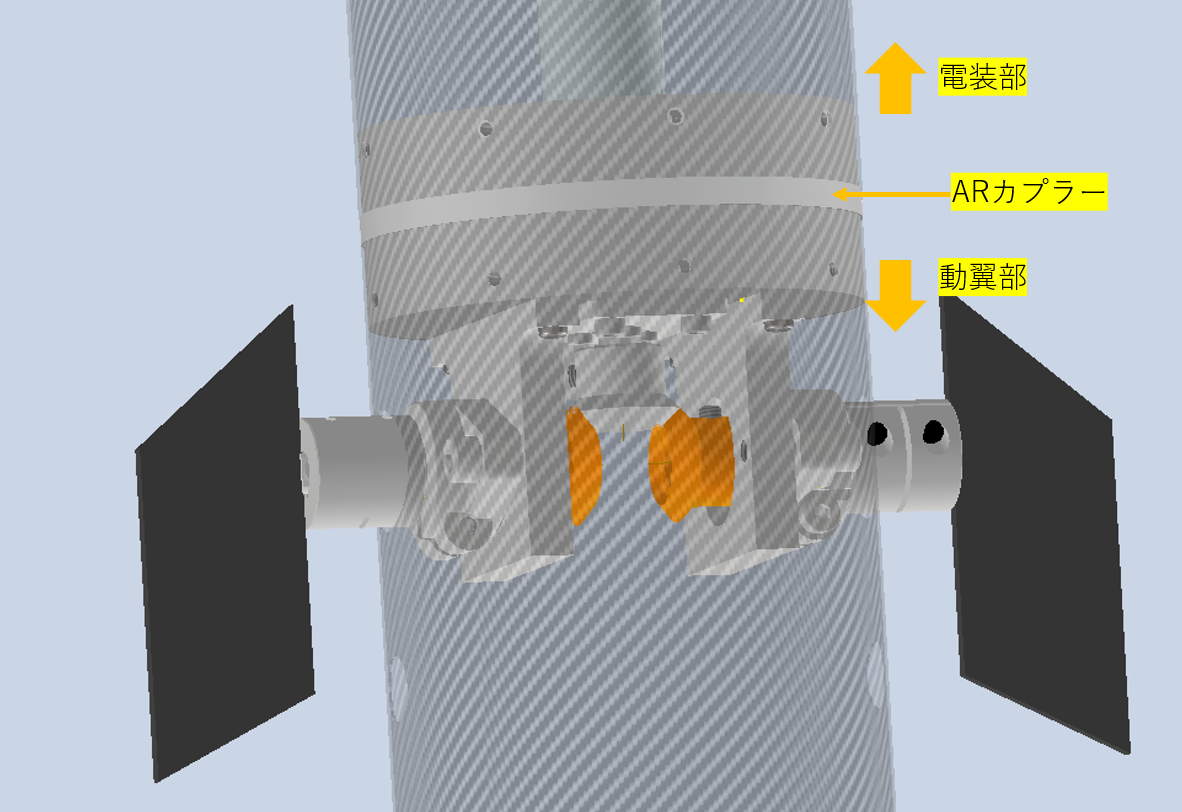
\includegraphics[scale = 0.3]{pic_str/s_roll_all.png}
	\caption{動翼機構CAD図}
	\label{s_r_all}
\end{figure}

\begin{figure}[H]
	\centering
	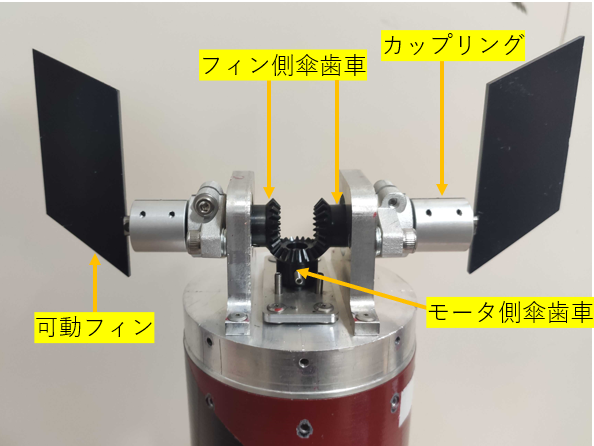
\includegraphics[scale = 0.6]{pic_str/s_r_pic.png}
	\caption{動翼機構}
	\label{s_r_pic}
\end{figure}

\begin{figure}[H]
	\centering
	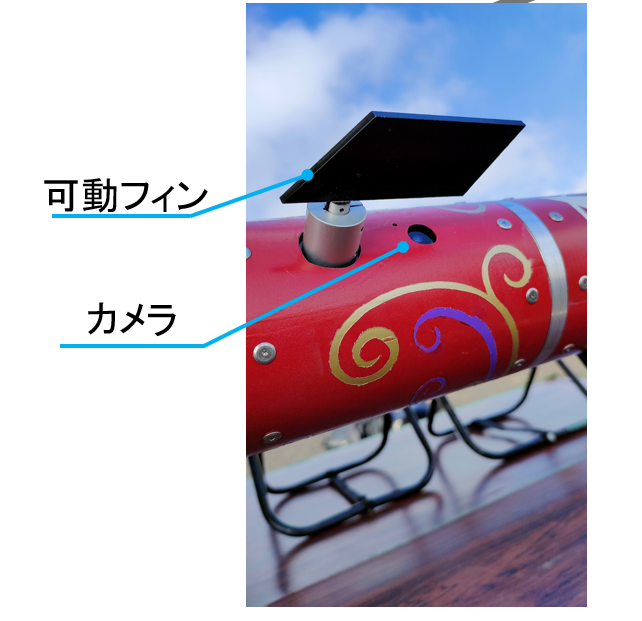
\includegraphics[scale = 0.55]{pic_str/s_r_outer_2.png}
	\caption{動翼部外形}
	\label{s_r_outer}
\end{figure}

傘歯車を介して、モータの回転を左右2枚の可動フィンに伝える機構になっている。
このような機構にすることで、2枚の可動フィンが連動し、かつ同じ量だけ回転するようにしている。\footnote{
	傘歯車を使用せず、左右にサーボモータを設置しフィンを回転させる方法も検討したが、高精度の制御ができるモータを使用したい、左右2つのフィン回転量が等しいことを担保したい、という2点よりこの機構を採用した。
	代わりに傘歯車のバックラッシが小さく、かつ摩擦補償が小さい機構の製作が必要となった。}
以下に特記点を示す。
\begin{itemize}
	\item フィン側傘歯車と可動フィンは連動して回転するようになっているが、左右2枚の可動フィンの位相を合わすために、カップリングを設置している。
	      現地組立では水準器を使用し、2枚の可動フィンと機軸の水平度を測ることでフィン位相を合わせた。
	      \\
	\item 電装計器の誤作動、電源喪失、ピトー管からの対気速度値異常などが原因で可動フィンが想定より多く回転してしまい、機体の姿勢が不安定になってしまう可能性がわずかながらある。この状況を防ぐため、フィンの回転制御角を物理的に制限する機構を搭載している。この機構のCAD図を図\ref{s_r_kadouiki}に示す。
	      \begin{figure}[H]
		      \centering
		      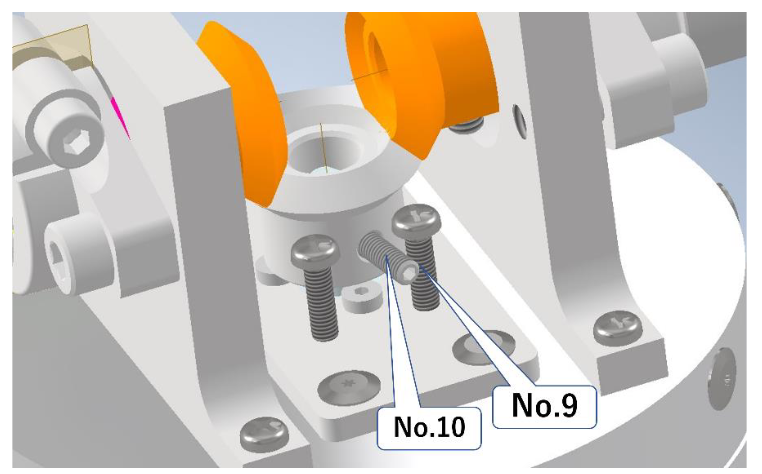
\includegraphics[scale = 0.5]{pic_str/s_r_kadouiki.png}
		      \caption{回転角制御機構}
		      \label{s_r_kadouiki}
	      \end{figure}
	      モータと傘歯車を締結しているイモネジ(No.10)を仕様より長いものを使用し、回転角が中央\footnote{2つ設置してあるネジ(No.9)から等距離の地点。}から$\pm \SI{15}{deg}$ を超えるとネジ(No.9)に当たり、止まるようになっている。
	      また、制御開始時にイモネジが中央に位置していないといけないが、カップリングの印をつけることで、フィン位相をあわせる際にイモネジが中央位置かどうかをわかるようにした。
	      また、イモネジの正しい使い方をしていないため、通常使用時から緩むようになっていたが、ネジロックを使用することで緩まないようにした。
	      \\
	\item 前述の通り、バックラッシを調整できるような設計を行った。主に加工誤差が原因で、傘歯車を設計値通りの場所に設置することができないため、製作後に傘歯車の位置をワッシャーとシムリングを挟むことでで調整できるようにした。
	      実際に\SI{0.1}{mm}ごとに傘歯車の位置を調整していき、バックラッシが小さくなり、かつ摩擦補償が小さくなる位置を決定した。
	      \\
	\item 図\ref{s_r_outer}に示したように、動翼のすぐ下にカメラを設置した。これは飛行中に動翼が正常に動作していることを確認するため、及びロールしない映像を撮影するためである。
\end{itemize}


\newpage
\subsection{テールコーン}
\label{tale}

エンジン排気の流れを整えることを目的として、機体後端にテールコーンを設置した。
テールコーン付近の断面図を図\ref{s_tale_num}に、主な構成部品を表\ref{s_tale_table}に示す。
また、テールコーンの図面を図\ref{s_tale_zumen}に示す。

\begin{figure}[H]
	\centering
	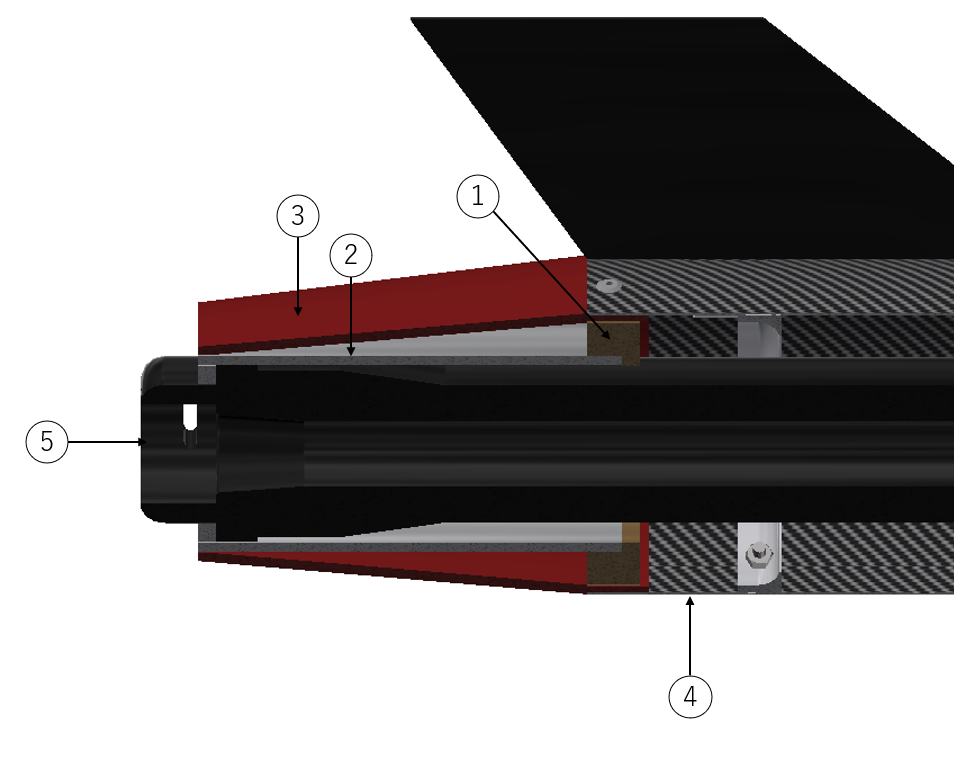
\includegraphics[scale = 0.4]{pic_str/s_talecorn_num.png}
	\caption{テールコーン付近断面図}
	\label{s_tale_num}
\end{figure}

\begin{table}[H]
	\centering
	\caption{テールコーン部品表}
	\begin{tabular}{ccc} \toprule
		No. & 名称       & 材質、型番         \\ \midrule
		1   & エンジン受け1  & A5052         \\
		2   & エンジン受け2  & A5052         \\
		3   & テールコーン   & ABS           \\
		4   & エンジンチューブ & CFRP          \\
		5   & エンジン     & HyperTEK J250 \\ \bottomrule
	\end{tabular}
	\label{s_tale_table}
\end{table}

\begin{figure}[H]
	\centering
	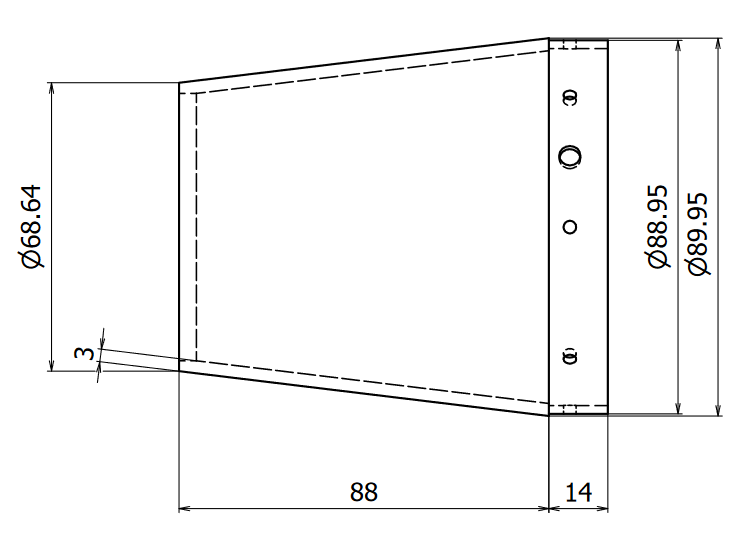
\includegraphics[scale = 0.6]{pic_str/s_talecorn_zumen.png}
	\caption{テールコーン図面}
	\label{s_tale_zumen}
\end{figure}

\newpage
\section{電装系開発概要}
\subsection{電装系全体概要}

電装タワー上段からGPS基板、開放基板、ミッション基板の3つの基板を搭載した。
GPS基板と開放基板はマイコンにSTM32-F446RET6を、ミッション基板はESP32を搭載した。
記憶素子はSPI flashであるS25FL127を搭載した。基板動作用電源としてCR123Aを4個、動翼用電源としてLiFeバッテリーを搭載した。
電装系全体の概要図を図\ref{fig:avi_all}に、基板ごとの役割を表\ref{tab:avi_ref}に示す。
また、実際の電装タワーの外観を図\ref{fig:avi_tower}に示す。

\begin{figure}[H]
	\centering
	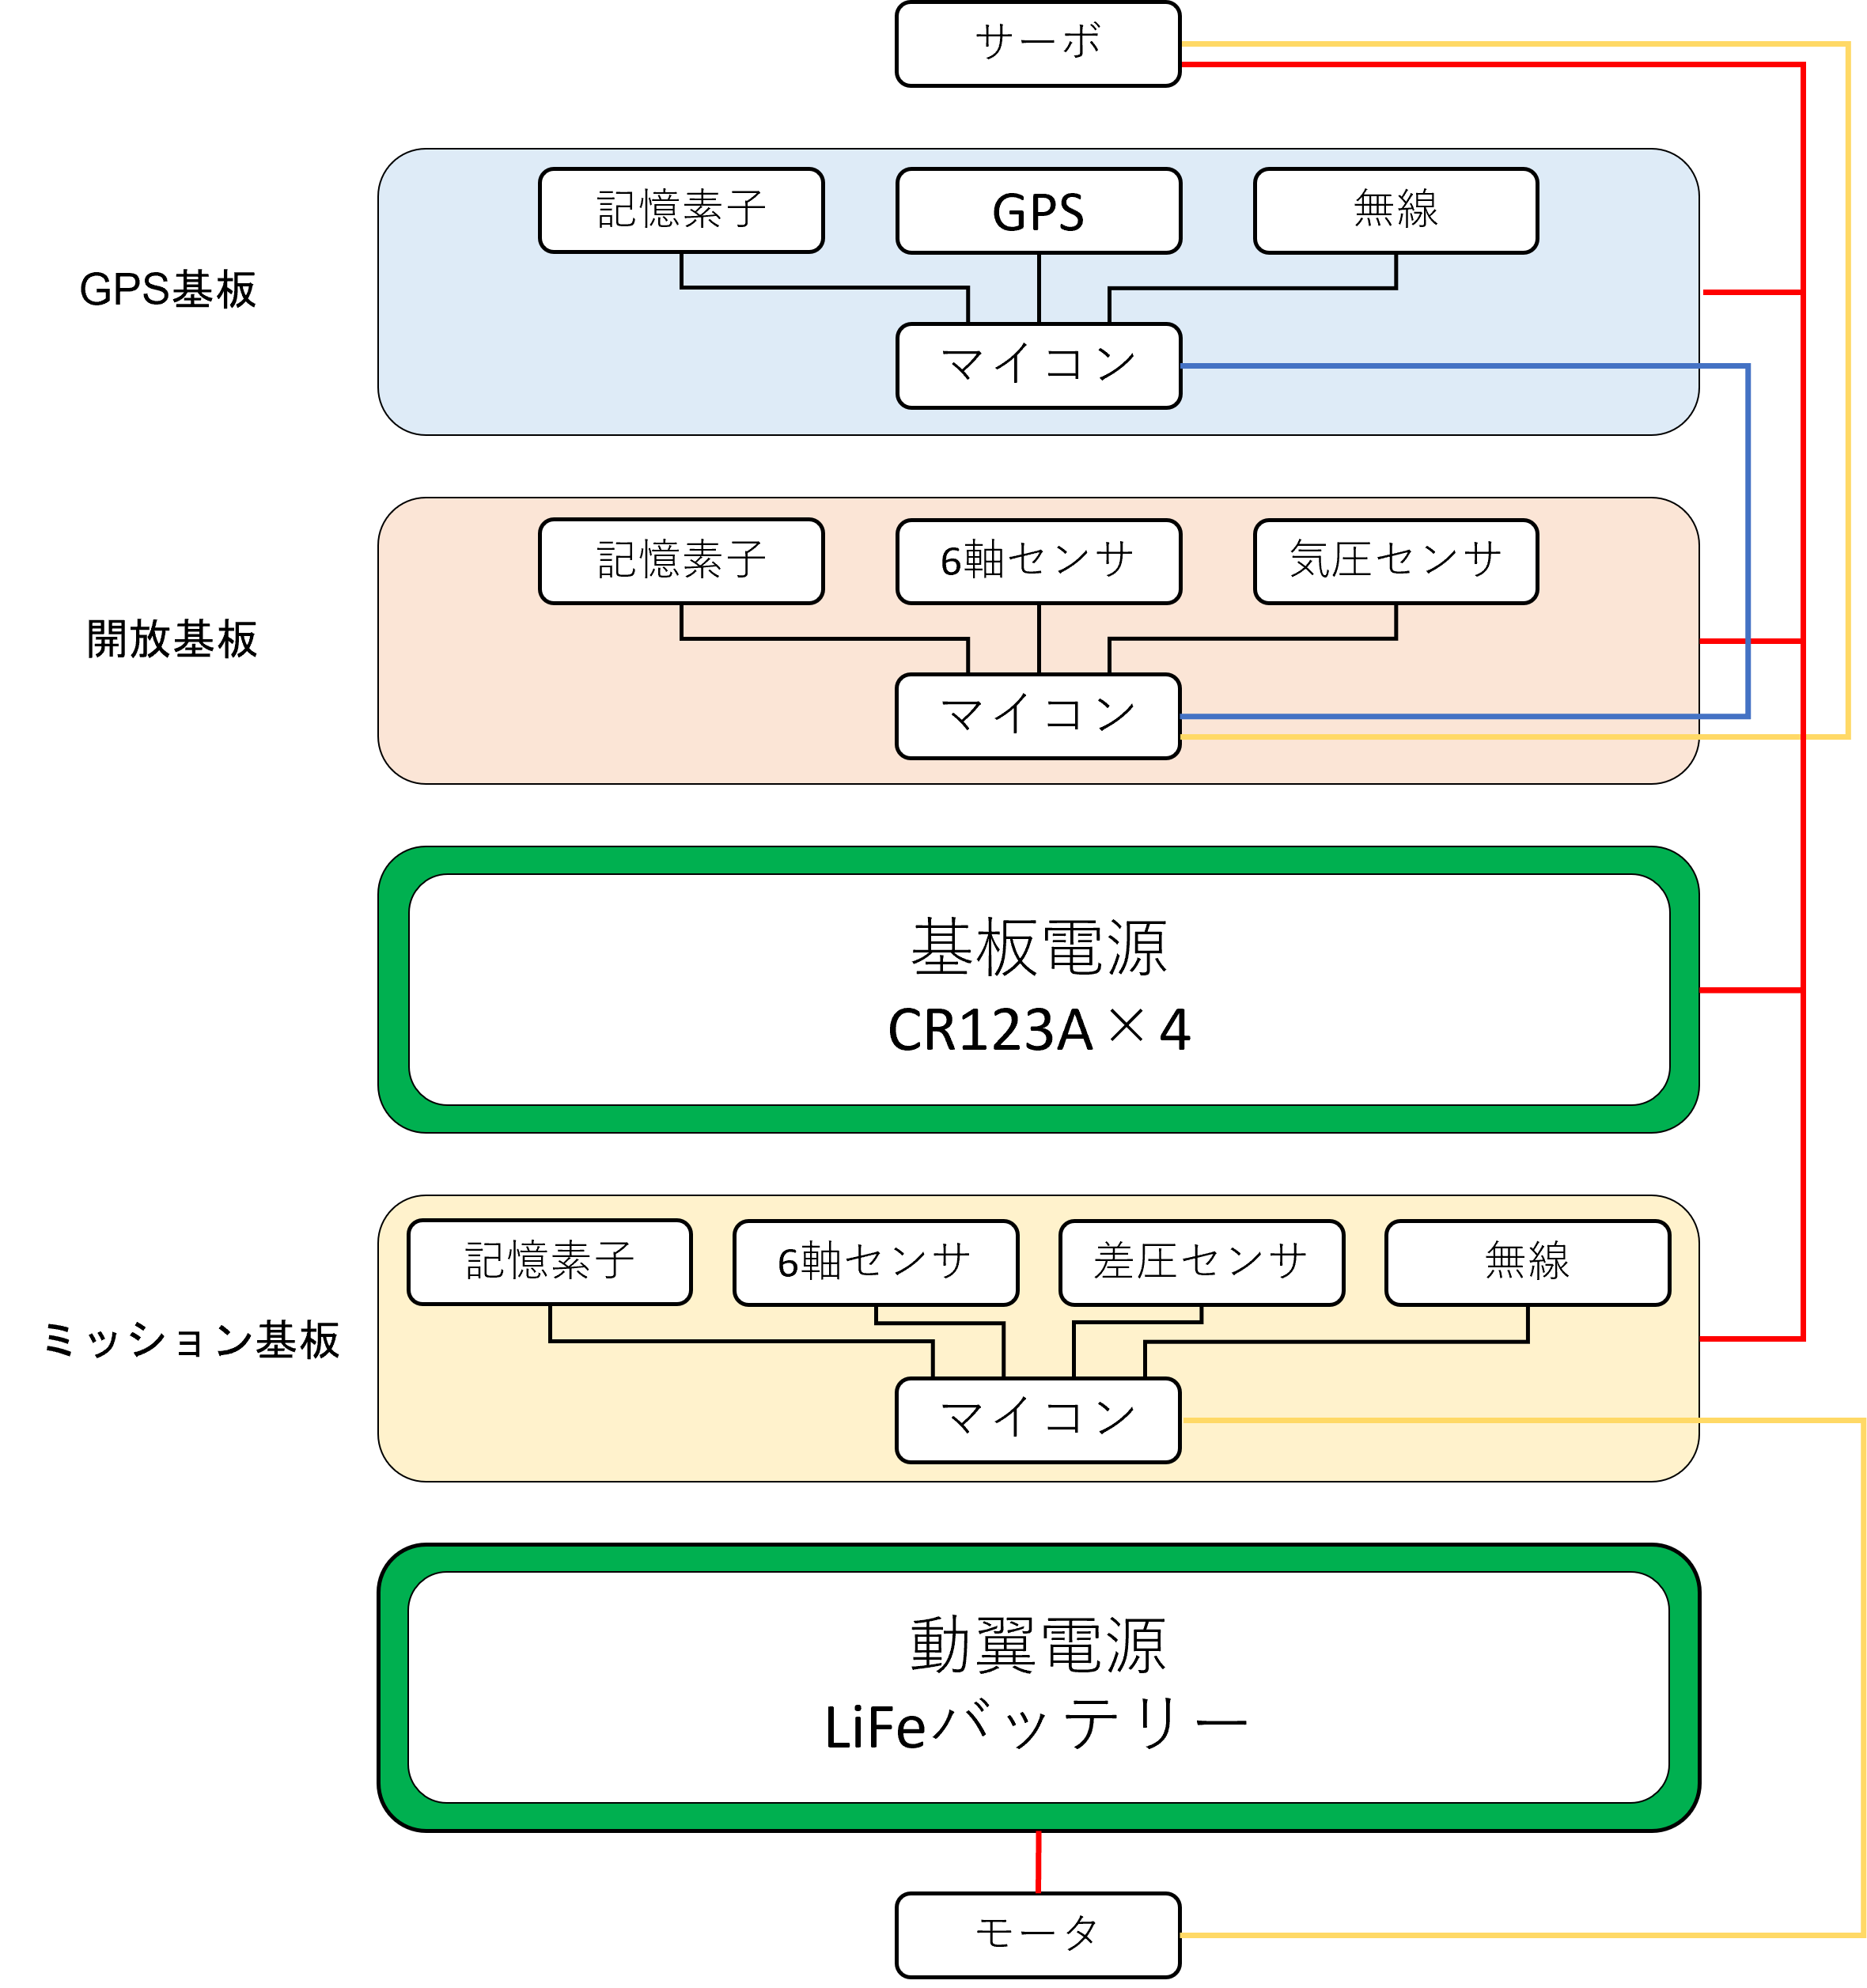
\includegraphics[width=0.8\linewidth]{pic_summary/avi_all.png}
	\caption{電装系全体の概要}
	\label{fig:avi_all}
\end{figure}


\begin{table}[H]
	\centering
	\caption{基板ごとの役割}
	\begin{tabular}{cccc} \toprule
		基板      & 役割         \\ \midrule
		GPS基板   & GPSのダウンリンク \\
		開放基板    & 減速機構の制御    \\
		ミッション基板 & 動翼の制御      \\
		\bottomrule
	\end{tabular}
	\label{tab:avi_ref}
\end{table}

\begin{figure}[H]
	\centering
	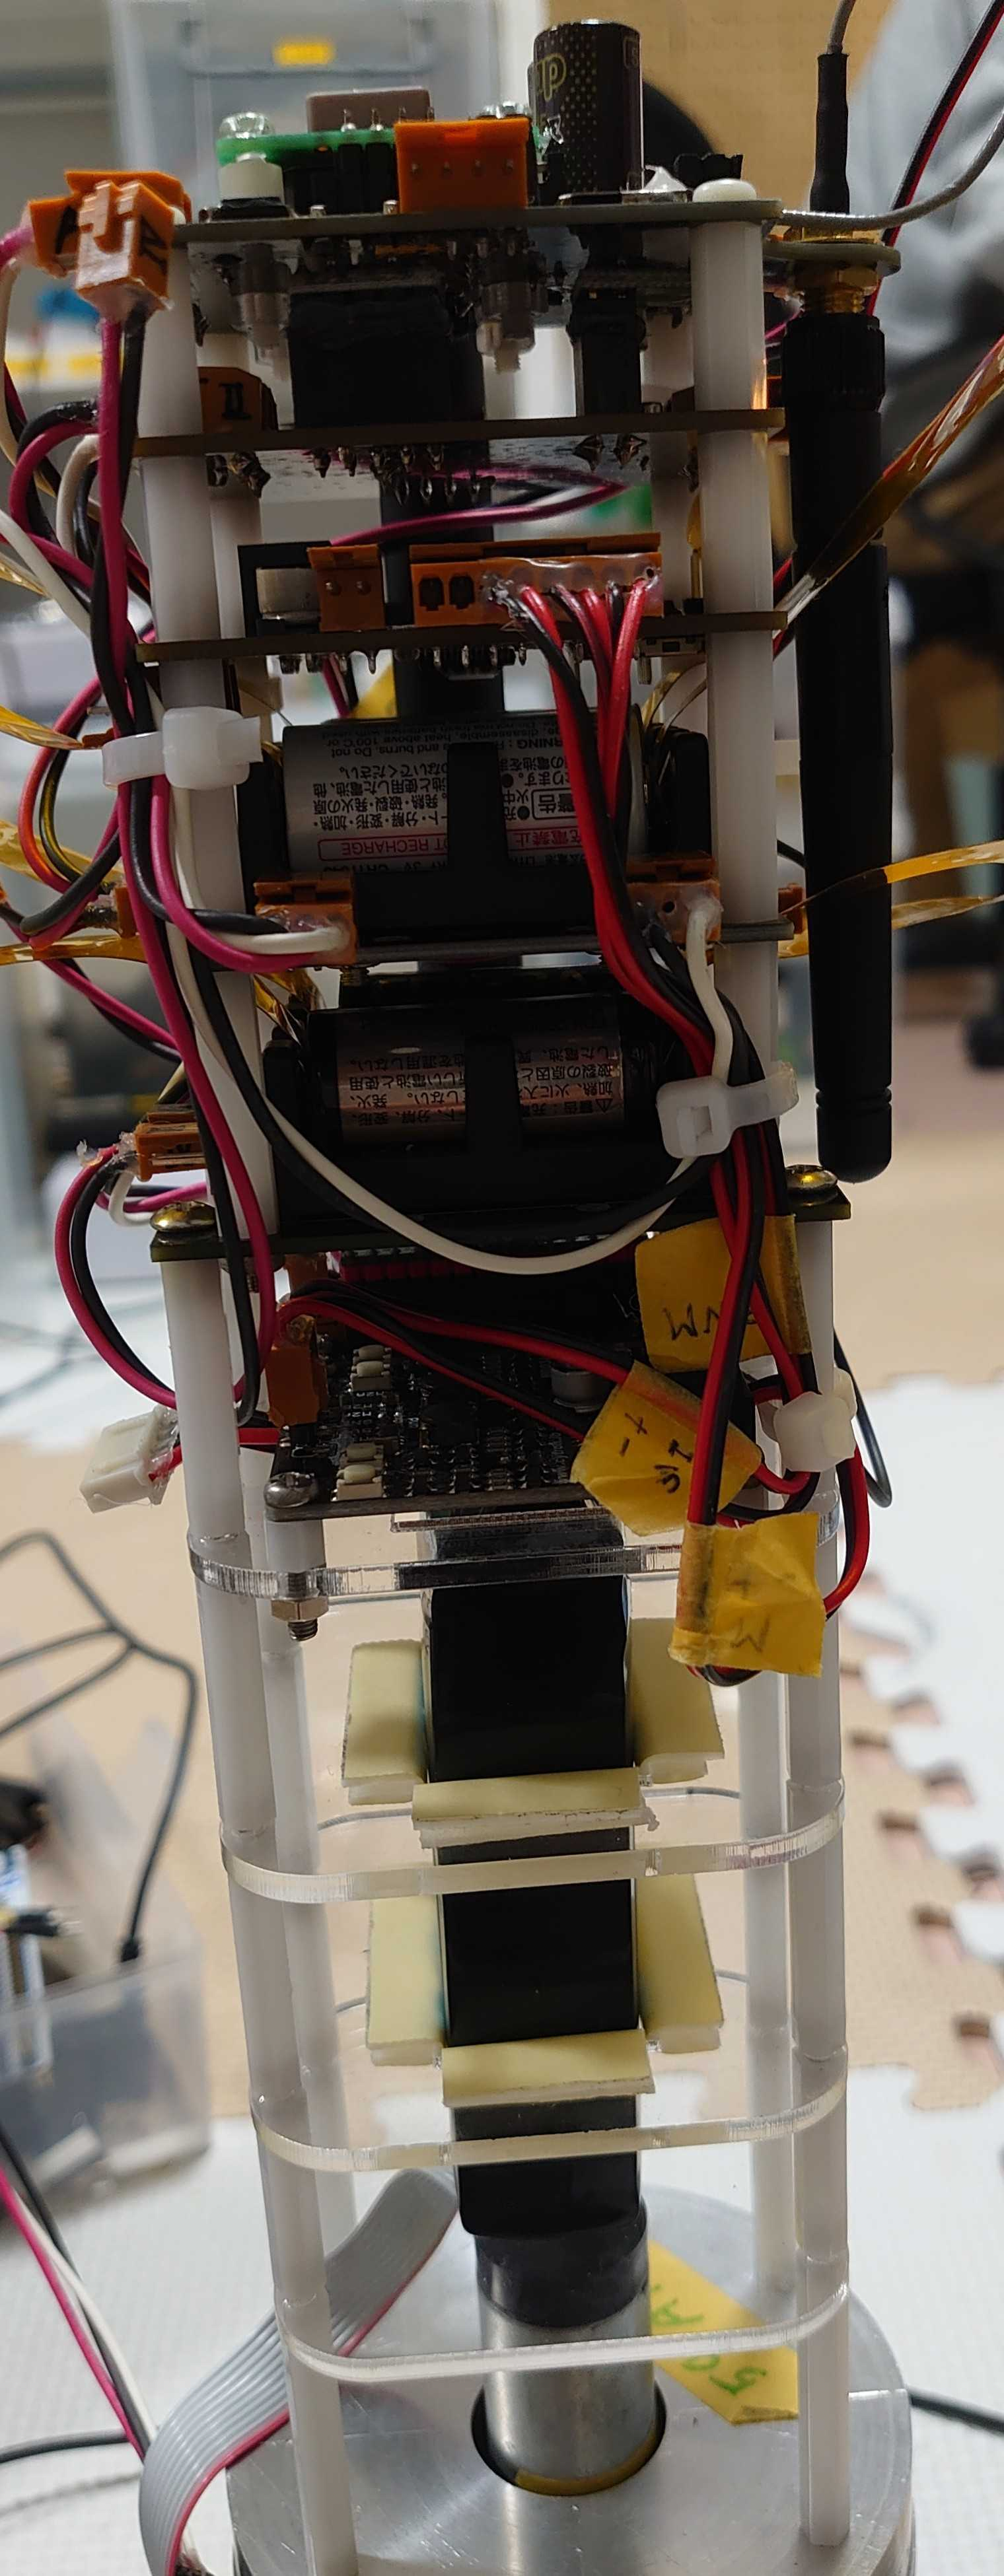
\includegraphics[width=0.25\linewidth]{pic_avi/avi_tower.JPG}
	\caption{電装タワー外観}
	\label{fig:avi_tower}
\end{figure}

\subsection{各基板の構成}

\subsubsection{GPS基板}
\begin{itemize}
	\item 役割
	      \begin{itemize}
		      \item GPS位置座標の取得、記録
		      \item 無線通信による開放基板へのコマンド操作
	      \end{itemize}

	\item 搭載モジュールの詳細(表\ref{tab:com_detail})
	      \begin{table}[H]
		      \centering
		      \caption{GPS基板のセンサ等詳細}
		      \begin{tabular}{cccc} \toprule
			      センサ等種類 & 型番           & サンプリングレート (\si{Hz}) & 測定範囲 \\ \midrule
			      GPS    & AE-GYSFDMAXB & 10                  & -    \\
			      無線     & TWE-Lite-RED & -                   & -    \\
			      \bottomrule
		      \end{tabular}
		      \label{tab:com_detail}
	      \end{table}
\end{itemize}

\subsubsection{開放基板}
\begin{itemize}
	\item 役割
	      \begin{itemize}
		      \item 減速機構の開放動作
		      \item \SI{1000}{Hz}での加速度、角速度のロギング
		      \item \SI{50}{Hz}での気圧のロギング
	      \end{itemize}

	\item 搭載モジュールの詳細(表\ref{tab:para_detail})
	      \begin{table}[H]
		      \centering
		      \caption{開放基板のセンサ等詳細}
		      \begin{tabular}{cccc} \toprule
			      センサ等種類 & 型番       & サンプリングレート (\si{Hz}) & 測定範囲                          \\ \midrule
			      加速度    & MPU-9250 & 1000                & \SI{+-16}{G}                  \\
			      角速度    & MPU-9250 & 1000                & \SI{+-2000}{deg/s}            \\
			      気圧     & LPS-22HB & 50                  & \SI{260}{hPa}から\SI{1260}{hPa} \\
			      \bottomrule
		      \end{tabular}
		      \label{tab:para_detail}
	      \end{table}

	\item 離床検知条件
	      \begin{enumerate}
		      \item 各軸それぞれの加速度センサの直近の値20回分(=0.02秒間分)の平均値を$\bar{a}_x,\,\bar{a}_y,\,\bar{a}_z$とする。このとき、
		            \begin{equation}
			            \sqrt{{\bar{a}_x}^2 + {\bar{a}_y}^2 + {\bar{a}_z}^2} > \SI{2}{G}
		            \end{equation}
		            を50回連続で満たしたとき
		      \item 気圧センサの直近の値5回分(=0.1秒間分)の平均を取り、この値が前回の値より \SI{0.1}{hPa}以上低い状態が1秒間連続したとき
	      \end{enumerate}
	      上記のうちいずれか1つを満たしたとき、その1秒前を離床時刻とする。

	\item 頂点検知条件
	      \begin{enumerate}
		      \item 離床検知から3秒以上経過していること
		      \item 離床から10.65秒後
		      \item 0.1秒ごとに気圧センサの値の5回分の平均値を取り、この平均値が前回の平均値より高い状態が1秒間連続すること
	      \end{enumerate}
	      上記のうちAを満たし、かつB、Cのうち1つの条件を満たしたときに減速機構を開放する。
\end{itemize}


\subsubsection{ミッション基板}
\begin{itemize}
	\item 役割
	      \begin{itemize}
		      \item 動翼を用いたロール制御
		      \item \SI{500}{Hz}での加速度、角速度、対気速度のロギング
	      \end{itemize}

	\item 搭載モジュールの詳細(表\ref{tab:mission_detail})
	      \begin{table}[H]
		      \centering
		      \caption{GPS基板のセンサ等詳細}
		      \begin{tabular}{cccc} \toprule
			      センサ等種類 & 型番              & サンプリングレート (\si{Hz}) & 測定範囲               \\ \midrule
			      加速度    & MPU-9250        & 500                 & \SI{+-16}{G}       \\
			      角速度    & MPU-9250        & 500                 & \SI{+-2000}{deg/s} \\
			      差圧計    & HSCDRRN100MDSA3 & 500                 & \SI{+-100}{mbar}   \\
			      無線     & TWE-Lite-RED    & -                   & -                  \\
			      \bottomrule
		      \end{tabular}
		      \label{tab:mission_detail}
	      \end{table}
\end{itemize}

\subsection{動翼を用いたロール制御}
\subsubsection{概要}
エンジン燃焼終了後からパラシュート開傘までの間、機体のロール角を一定値に保つ制御を行った。エンコーダ付きDCモータを用いて動翼の角度を制御し、空力によって発生するロールモーメントを用いて制御した。
\subsubsection{ハードウェア構成}
動翼角度を制御するために、MAXON社製のエンコーダ付きギアモータを使用した。モータはA-max22(製品番号110158)を使用した。
良好な制御特性を得るために慣性モーメントの小さいコアレスモータを用いることとし、比較的価格が安いA-maxシリーズを採用した。
ギアヘッドは、減速比29.16のプラネタリギアを用いた。十分なトルクと動翼回転速度を両立する減速比を採用した。低バックラッシ品の採用は、価格を考慮し断念した。
エンコーダは、512パルス/回転で2相のインクリメンタルエンコーダを用いた。動翼角度の分解能は、4逓倍を用いて$360/512/4/29.16\simeq \SI{0.006}{deg}$である。
使用したセンサの詳細は表\ref{tab:mission_detail}に記述した。動翼機構の詳細は\ref{douyoku}節に記述した。
\subsubsection{制御則}
図\ref{fig:ブロック線図}に対気速度がある値$v$のときの、制御器と制御対象をモデル化したブロック線図を示す。
\begin{figure}[H]
	\centering
	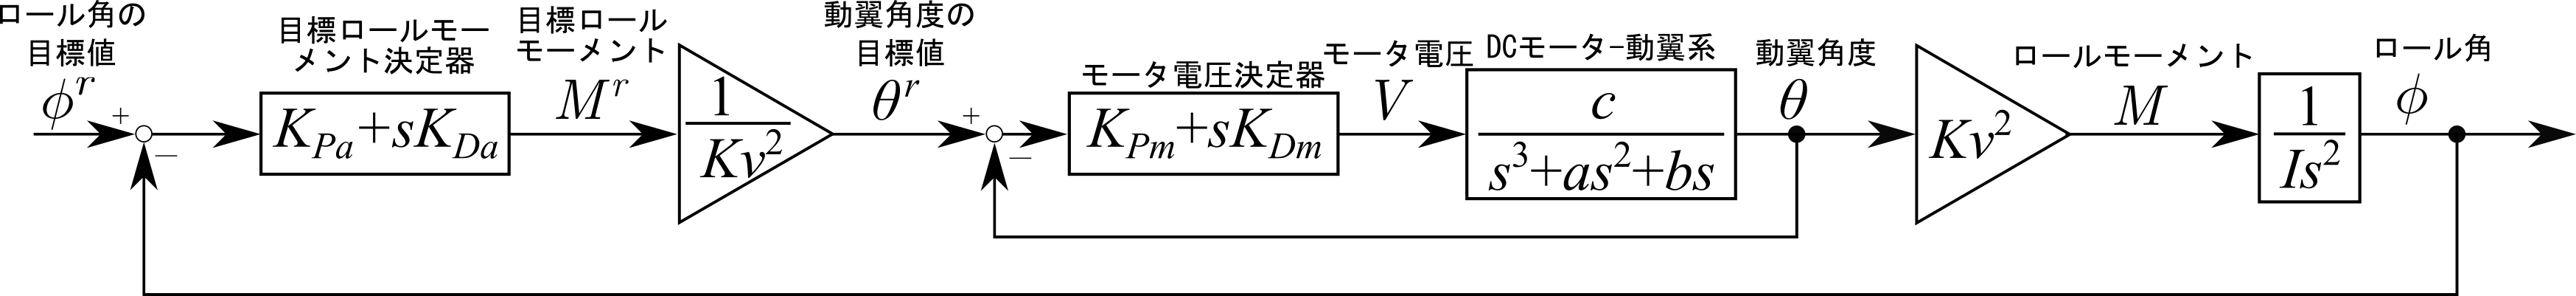
\includegraphics[width=0.95\linewidth]{pic_avi/block_diagram.png}
	\caption{ブロック線図}
	\label{fig:ブロック線図}
\end{figure}
対気速度はピトー管により計測される。制御対象であるロール角とロールモーメントの関係は、
\begin{equation}
	I\ddot\phi=M
\end{equation}
によりモデル化する。ただし$I$はロール方向の慣性モーメント、$\phi$はロール角、$M$は動翼が発生させるロールモーメントである。
動翼が発生させるロールモーメントの目標値$M^r$は、目標ロールモーメント決定器がPD制御を用いて決定する。$K_{Pa}$がPゲイン、$K_{Da}$がDゲインである。
エンコーダ付きギアモータの出力を傘歯車を介して伝えることで、2枚の動翼を駆動する。これらの機構を合わせてモータ-動翼系と呼称する。モータ-動翼系を
\begin{equation}
	\frac{V(s)}{\theta(s)}=\frac{c}{s^3+as^2+bs}
\end{equation}
によりモデル化する。ただし、$V$はモータに印加する電圧、$\theta$は動翼角度である。$a、b、c$は定数であり、システム同定実験に基づき決定する。
$V$は、モータ電圧決定器がPD制御を用いて決定する。$K_{Pm}$がPゲイン、$K_{Dm}$がDゲインである。動翼角度$\theta$とロールモーメント$M$, 対気速度$v$の関係は、
\begin{equation}
	M=K\theta v^2
\end{equation}
で表される。ただし$K$は定数であり、流体シミュレーションにより求める.目標ロールモーメント$M^r$が与えられたとき、これを$Kv^2$で除算し、動翼角度の目標値$\theta^r$を決定する。\par
以上のモデル化を行ったとき、ロール角の目標値$\phi^r$からロール角$\phi$への開ループ伝達関数$G_o(s)$と閉ループ伝達関数$G_c(s)$はそれぞれ
\begin{equation}
	\begin{split}
		G_{o}(s)&=\frac{cK_{Da}K_{Dm}s^2+c\left(K_{Pa}K_{Dm}+K_{Pm}K_{Da}\right)s+cK_{Pa}K_{Pm}}{Is^5+aIs^4+\left(b+cK_{Dm}\right)Is^3+cK_{Pm}Is^2}\\
		G_{c}(s)&=\frac{cK_{Da}K_{Dm}s^2+c\left(K_{Pa}K_{Dm}+K_{Pm}K_{Da}\right)s+cK_{Pa}K_{Pm}}{Is^5+aIs^4+\left(b+cK_{Dm}\right)Is^3+c\left(K_{Pm}I+K_{Da}K_{Dm}\right)s^2+c(K_{Pa}K_{Dm}+K_{Pm}K_{Da})s+cK_{Pa}K_{Pm}}
	\end{split}
\end{equation}
と求まる。十分なゲイン余裕と位相余裕を有し、過去のデータの分析をもとに想定した外乱ロールモーメントがある場合に目標ロール角に収束可能な制御ゲインを決定した。\par
制御則を実装するにあたり、ロール角は角速度センサの値を用いて求めた。ロール角速度も同様に求め、カットオフ周波数50 Hzの1次のローパスフィルタを施した。
動翼角度はエンコーダの値を用いて求めた。動翼角速度は動翼角度の前時刻との差分を用いて求め、カットオフ周波数50 Hzの1次のローパスフィルタを施した。
対気速度はピトー管の値を用いて求め、カットオフ周波数20 Hzの1次のローパスフィルタを施した。

\newpage
\section{打上結果}
以下の表\ref{tab:utiage_shogen}に打上げ時の気温や時刻などのデータをまとめて示す。
\begin{table}[H]
	\centering
	\caption{打上げに関するデータ}
	\label{tab:utiage_shogen}
	\begin{tabular}{lcr}
		\hline
		名称   & 単位                    & \multicolumn{1}{c}{値} \\
		\hline
		日付   &                       & 2022/11/13            \\
		日時   &                       & 7:47                  \\
		気温   & \SI{}{\degreeCelsius} & 18.62                 \\
		気圧   & \SI{}{hPa}            & 964.49                \\
		射点高度 & \SI{}{m}              & 430                   \\
		射点緯度 & \SI{}{deg}            & 北緯34.736139           \\
		射点経度 & \SI{}{deg}            & 東経139.421333          \\
		磁気偏向 & \SI{}{deg}            & 7.53(西偏)              \\
		風向   & \SI{}{deg}            & 180                   \\
		風速   & \SI{}{m/s}            & 3.0                   \\
		\hline
	\end{tabular}
\end{table}

\subsection{打上スケジュール}
以下の表\ref{tab:search_1nitime}に1日目の実際のスケジュールを示す。

\begin{table}[H]
	\centering
	\caption{1日目の打上げスケジュール}
	\begin{tabular}{cl} \toprule
		時刻    & \multicolumn{1}{c}{イベント} \\ \midrule
		8:00  & C-59J組立開始                \\
		9:00  & C-59J組立終了                \\
		12:00 & C-59J点火点に搬入              \\
		13:00 & C-61J打上げ、GSEトラブル         \\
		16:50 & 本部撤収                     \\
		19:00 & GSEトラブルの原因究明開始           \\
		23:45 & 原因究明・対策・試験終了             \\
		\bottomrule
	\end{tabular}
	\label{tab:search_1nitime}
\end{table}

以下の表\ref{tab:search_2nitime}に2日目の実際のスケジュールを示す。
\begin{table}[H]
	\centering
	\caption{2日目の打上げスケジュール}
	\begin{tabular}{cl} \toprule
		時刻    & \multicolumn{1}{c}{イベント} \\ \midrule
		4:20  & C-59J組立開始                \\
		4:40  & ボンベ開栓より前のGSE展開完了         \\
		6:00  & C-59J点火点到着               \\
		6:30  & CORE X                   \\
		6:40  & 安全確認終了                   \\
		6:40  & GSE最後のガスあり試験開始           \\
		6:50  & 機体移動 \&\ ランチャー整備         \\
		6:55  & ランチャー挿入開始                \\
		7:05  & ステム挿入開始                  \\
		7:15  & ランチャー立上開始                \\
		7:37  & 総員退避完了                   \\
		7:38  & ミッション基板でリブート発生           \\
		7:40  & 諸元入力のため射点に接近             \\
		7:42  & 点火シーケンスへの移行許可            \\
		7:47  & C-59J X                  \\
		8:35  & ドローンによってC-59J発見          \\
		8:45  & 捜索隊によって目視でC-59J確認・回収     \\
		10:00 & 本部撤収                     \\
		\bottomrule
	\end{tabular}
	\label{tab:search_2nitime}
\end{table}

\subsubsection{GSE展開のタイムスケジュール}
2日目のGSE展開の詳細なタイムスケジュールを以下の表\ref{gse_time}に示す。
\begin{table}[H]
	\centering
	\caption{GSE展開スケジュール}
	\begin{tabular}{cl} \toprule
		時刻   & 作業内容               \\ \midrule
		3:30 & 裏砂漠入り口出発           \\
		4:15 & 射点到着・GSE展開開始       \\
		4:35 & 配管接続終了・ガスなし電磁弁試験開始 \\
		4:50 & ガスなし電磁弁動作試験完了      \\
		5:10 & ガスなしでの点火シーケンス試験開始  \\
		5:15 & ガスなしでの全ての試験完了      \\
		5:30 & 窒素ボンベ開栓            \\
		5:40 & 窒素を通しての電磁弁試験       \\
		6:00 & 亜酸化窒素ボンベ開栓         \\
		6:05 & 噴出試験               \\
		6:15 & 総員退避               \\
		6:40 & 総員退避解除             \\
		6:45 & 酸素ボンベ開栓            \\
		6:50 & 酸素電磁弁・イグナイタ同期試験    \\
		7:00 & GSE展開完了            \\
		\bottomrule
	\end{tabular}
	\label{gse_time}
\end{table}

今回のGSE展開は前日の問題の対策を講じたためいつもより時間を要することとなった。
しかし、展開の手際は非常に良く、問題となっていた中継基板も問題なく作動したため、非常にスムーズだったといえる。

\subsection{GSE各種試験}
1日目に行ったC-61J打上げの際に発生した中継基板の破壊事故を受けて、2日目のGSE展開では通常の試験に加えて破損した部分の重点的な試験を行った。
以下の表\ref{gse_mokuteki}行った試験の内容と目的、結果を示す。

\begin{table}[H]
	\centering
	\caption{GSE試験内容}
	\begin{tabular}{p{90mm}l} \toprule
		\multicolumn{1}{c}{試験内容}                                        & \multicolumn{1}{c}{結果} \\  \midrule
		充填時間を30秒間として、充填操作をして電磁弁の動作を確認する                                 & 電磁弁の動作を確認              \\ \midrule
		窒素ボンベを開栓し、充填時間を30秒として充填操作を行い電磁弁の動作を確認する。これを3度行った。               & 電磁弁の動作を確認              \\ \midrule
		亜酸化窒素ボンベも開栓し、噴出試験を行った。この試験は亜酸化窒素を大気開放する試験のため、電磁弁の操作時間は3秒程度であった。 & 亜酸化窒素の噴出と脱圧を確認         \\
		\bottomrule
	\end{tabular}
	\label{gse_mokuteki}
\end{table}

\subsection{ドローンによる捜索}
今回の打上実験ではドローンによる機体捜索を行った。本節では、ドローンによる捜索結果について簡単に述べる。
まずは、打上げ後の捜索のスケジュールを表\ref{tab:find}に示す。

\begin{table}[H]
	\centering
	\caption{X後の捜索のスケジュール}
	\begin{tabular}{cl} \toprule
		時刻   & \multicolumn{1}{c}{イベント} \\ \midrule
		7:47 & X                        \\
		7:59 & GPSによるC-59Jの落下位置推定完了     \\
		8:00 & 点火点から捜索隊1が推定落下位置に向けて出発   \\
		8:03 & 本部からドローンが推定落下位置に向けて出発    \\
		8:12 & 点火点から捜索隊2が推定落下位置に向けて出発   \\
		8:18 & ドローンのバッテリー切れで本部に一時撤退     \\
		8:20 & ドローンの予備バッテリーに交換し、再度出発    \\
		8:35 & ドローンによってC-59J発見          \\
		8:45 & 捜索隊によって目視でC-59J確認・回収     \\
		\bottomrule
	\end{tabular}
	\label{tab:find}
\end{table}

図\ref{fig:drone1}、\ref{fig:drone2}にドローンでの発見時の様子を示す。
なお、C-59J発見時におけるドローン写真を撮っていなかったため、C-61J発見時の写真を示している。

\begin{figure}[H]
	\centering
	\includegraphics[width=0.8\linewidth]{pic_search/drone1.png}
	\caption{ドローンからの発見時の様子1}
	\label{fig:drone1}
\end{figure}

\begin{figure}[H]
	\centering
	\includegraphics[width=0.8\linewidth]{pic_search/drone2.png}
	\caption{ドローンからの発見時の様子2}
	\label{fig:drone2}
\end{figure}

今回の打上実験では協賛企業である、株式会社天の技様のご厚意によりドローンを提供していただいた。
天の技様からドローンの提供がなければ、C-59Jの発見は困難だと推察される。
その理由として、想像以上に起伏が激しく見通しが悪かったことと、GPSの落下推定位置が実際の落下位置より\SI{60}{m}程度ずれていたことなどが挙げられる。

\newpage
\section{打上結果(構造・電装関係)}
\subsection{着地状況}
打上げでは正常に点火し、離床後10.2秒後に減速機構が作動し、正常にパラシュートが開傘した。
機体の着地状況を図\ref{s_tyakuti_pic}に示す。

\begin{figure}[H]
	\centering
	\includegraphics[scale = 0.08]{pic_str/s_tyakuti_pic.jpg}
	\caption{着地状況}
	\label{s_tyakuti_pic}
\end{figure}

落下の衝撃でアクリル製の固定フィンと可動フィンが機体から外れ、機体の周りに散らばっている様子が確認できた。
また、CFRP製のノーズコーンも落下の衝撃で割れていることが確認でき、チューブの塗装が一部めくれ傷がついていた。
しかし、それ以外の搭載計器やエンジン、動翼機構には問題無いことをその後確認した。


\subsection{データ回収について}
本節では、データの回収状況の説明と簡単な考察を行う。
詳細なデータ解析と事後シミュレーションについては\ref{sc:sim}章で行う。
\subsubsection{GPS基板}
離床から地上に落下する数秒前まではGPSデータの回収に成功した。
しかし、何らかの不具合により落下中の高度\SI{150}{m}時点でGPSからの信号が途絶しており、その原因は究明中である。

\subsubsection{開放基板}
\SI{1000}{Hz}で加速度・角速度、\SI{50}{Hz}で気圧データの回収に成功した。

\subsubsection{ミッション基板}
\SI{500}{Hz}で加速度・角速度、対気速度データの回収に成功した。

\subsubsection{離床検知}
打上動画及び各基板の機軸方向加速度データから、エンジンが振動燃焼を起こしていた可能性は大きいと考えられる。
開放基板のz軸方向(機軸方向、前方正)加速度の離床直前から燃焼終了後までの推移を図\ref{fig:az_data}に示す。
開放基板は直近20回分の加速度の平均値を算出し、\SI{50}{Hz}で加速度による離床検知を行った。
直近の加速度の平均値が1秒間連続して\SI{2}{G}を超えていれば離床と判断するため、振動燃焼による加速度のばらつきを吸収し、加速度で離床検知ができた。
\begin{figure}[H]
	\centering
	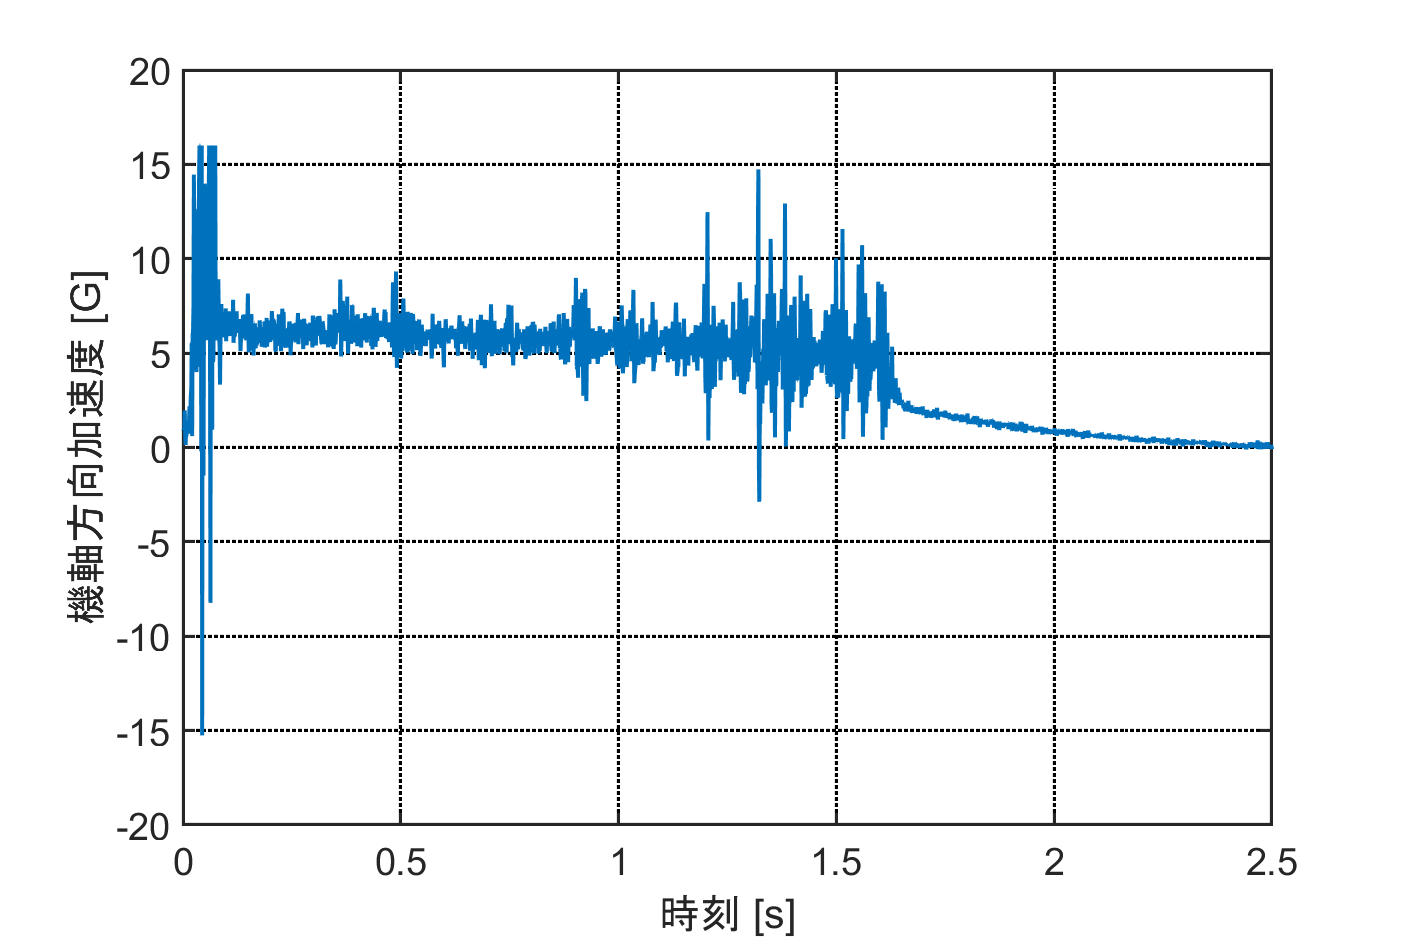
\includegraphics[width=0.8\linewidth]{pic_avi/59_6axis.png}
	\caption{機軸方向の加速度の時間推移(開放基板)}
	\label{fig:az_data}
\end{figure}

\subsubsection{ランチクリア速度}
まず、点火点から撮影した映像を元にランチクリア速度を算出したところ、約\SI{23.6}{m/s}であった。
一方、6軸センサで取得した加速度を積分して速度を求めたところ、ランチクリア速度は約\SI{23.2}{m/s}であった。
以上の結果より、ランチクリア速度は\SI{23}{m/s}程度であることがわかった。


\subsection{減速機構開放}
離床から10.2秒後に減速機構を開放した。タイマー条件ではなく、冗長系の気圧条件で頂点検知をして開放していたことがログから確認された。
実際の最高到達高度が\SI{353}{m}であったのに対し、予想最高到達高度が\SI{383}{m}だったため、頂点到達時刻が早くなったことが原因として考えられる。またデータからは頂点到達後約1.1秒後に減速機構に指令がなされていた。
頂点到達後1秒以内に減速機構に指令を出す想定でいたため、約0.1秒程度遅い展開となった。

\subsection{落下位置推定}
飛行中のGPSの電波を受信できたが、以下の図\ref{fig:GPS_data}に示すように、GPS最終受信地点は実際の落下地点と比較して直線距離で約\SI{60}{m}ずれてしまった。
大きなずれが生じてしまったのは、先に述べたように落下の途中までしかGPSデータをダウンリンクができなかったことが原因である。

\begin{figure}[H]
	\centering
	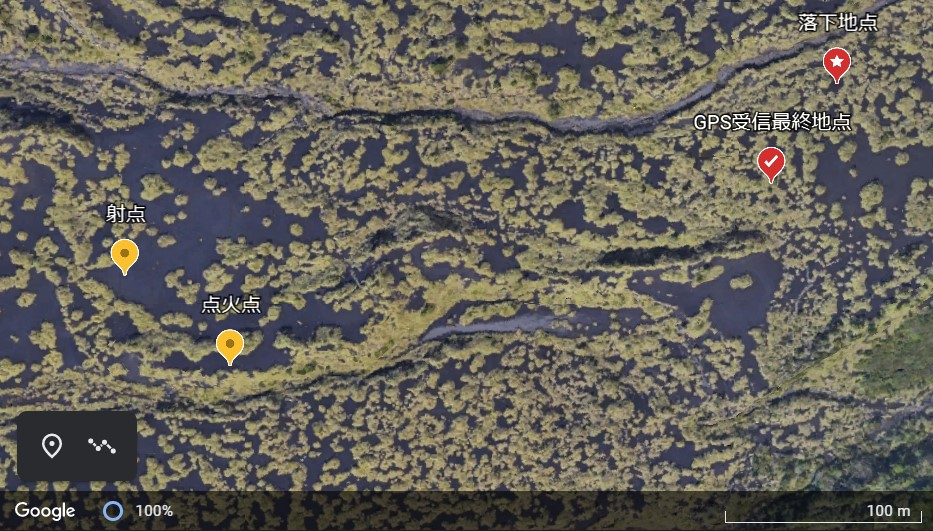
\includegraphics[width=0.8\linewidth]{pic_avi/GPS_data.jpg}
	\caption{GPS最終受信地点と実際の落下地点}
	\label{fig:GPS_data}
\end{figure}

\subsection{スイッチ機構}
\label{switch}
CREATEでは毎回の打ち上げで電池の持ちが問題となっていた。
そこで今回はスイッチ機構を搭載した。
図\ref{avi_switch_out}に示しているつまみ付きジャンパピンを抜くと電源が接続し、つけたままだと電源が遮断される仕組みとなっている。
内側は図\ref{avi_switch_in}のように3Dプリンターの治具と基板のモジュールでできており、配線がILGコネクタ―につながることで、電池基板とつないでいる。
1日目では9:30から16:00までの大半で電源を遮断していたが、開放基板とGPS基板の電圧は\SI{6.50}{V}から\SI{5.98}{V}に降下していた。
これはP型FETの回路内の抵抗の消費電力とサーボモータの待機電力が大きかったことが挙げられる。
次機体以降は外部給電を用いて電池の持ち時間に困らないシステムを構築したい。

\begin{figure}[H]
	\begin{tabular}{cc}
		\begin{minipage}[t]{0.45\hsize}
			\centering
			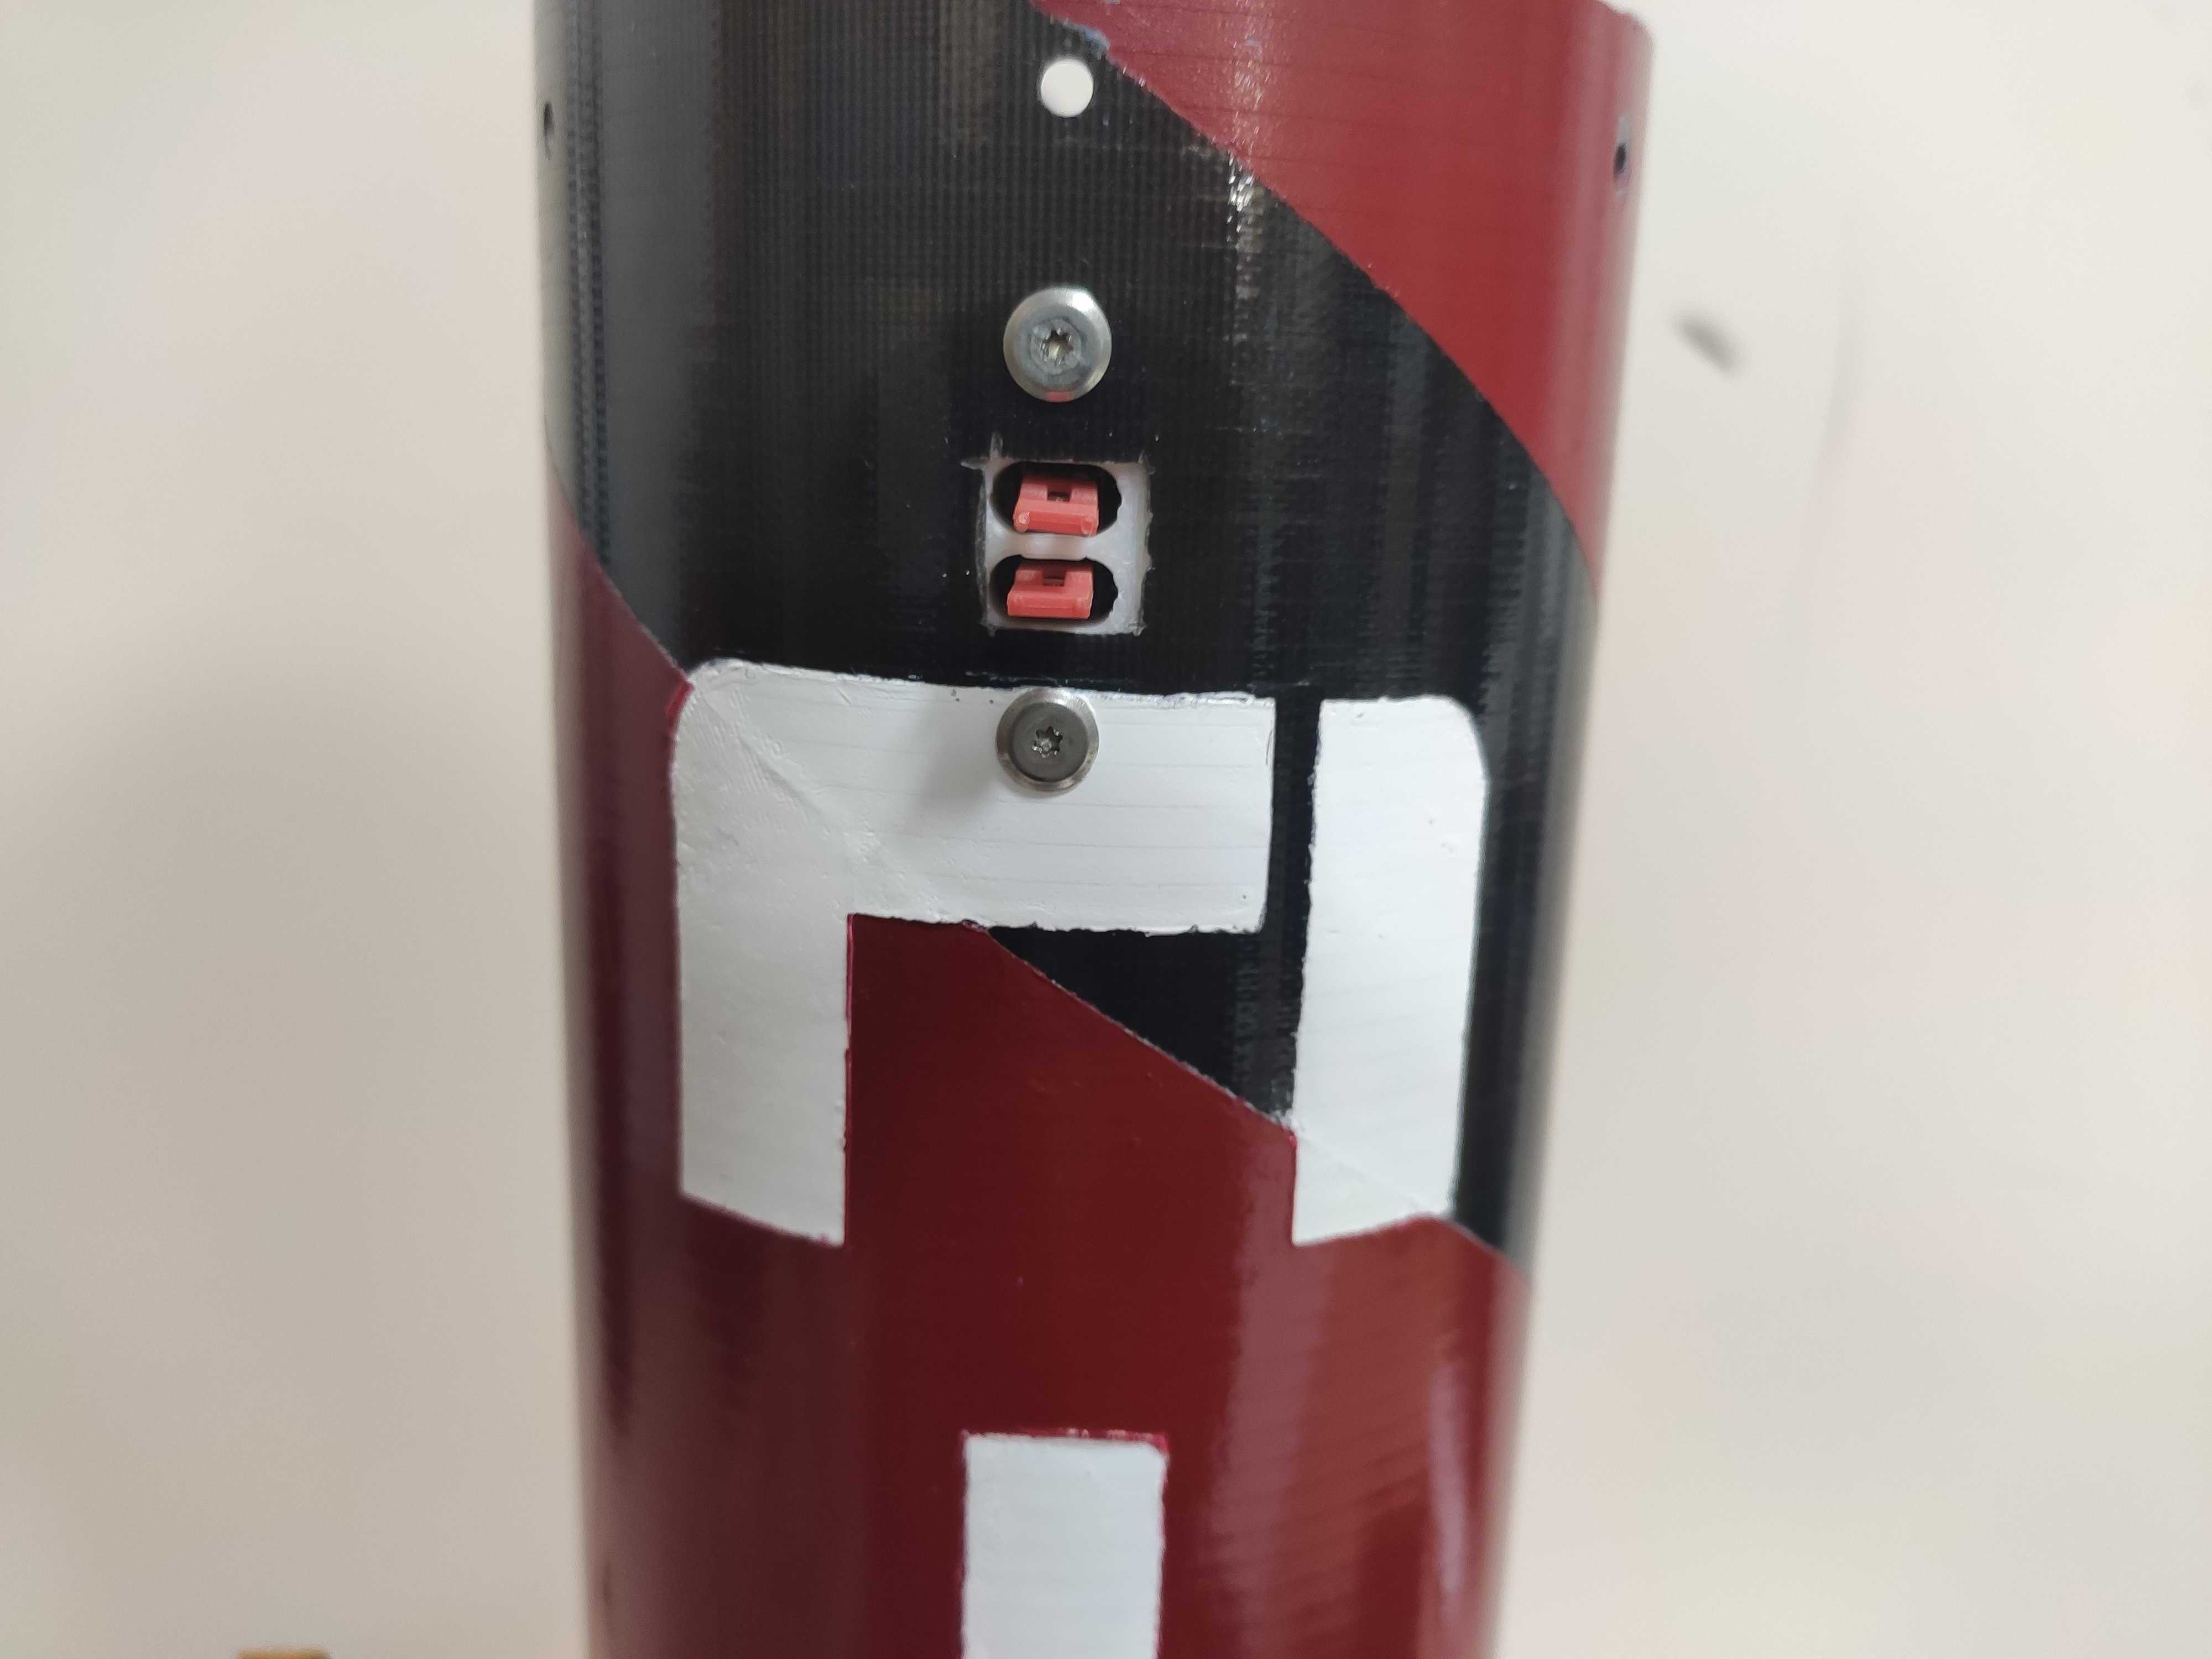
\includegraphics[scale = 0.05]{pic_avi/switch_out.jpg}
			\caption{スイッチ機構(外側)}\label{avi_switch_out}
		\end{minipage} &
		\begin{minipage}[t]{0.45\hsize}
			\centering
			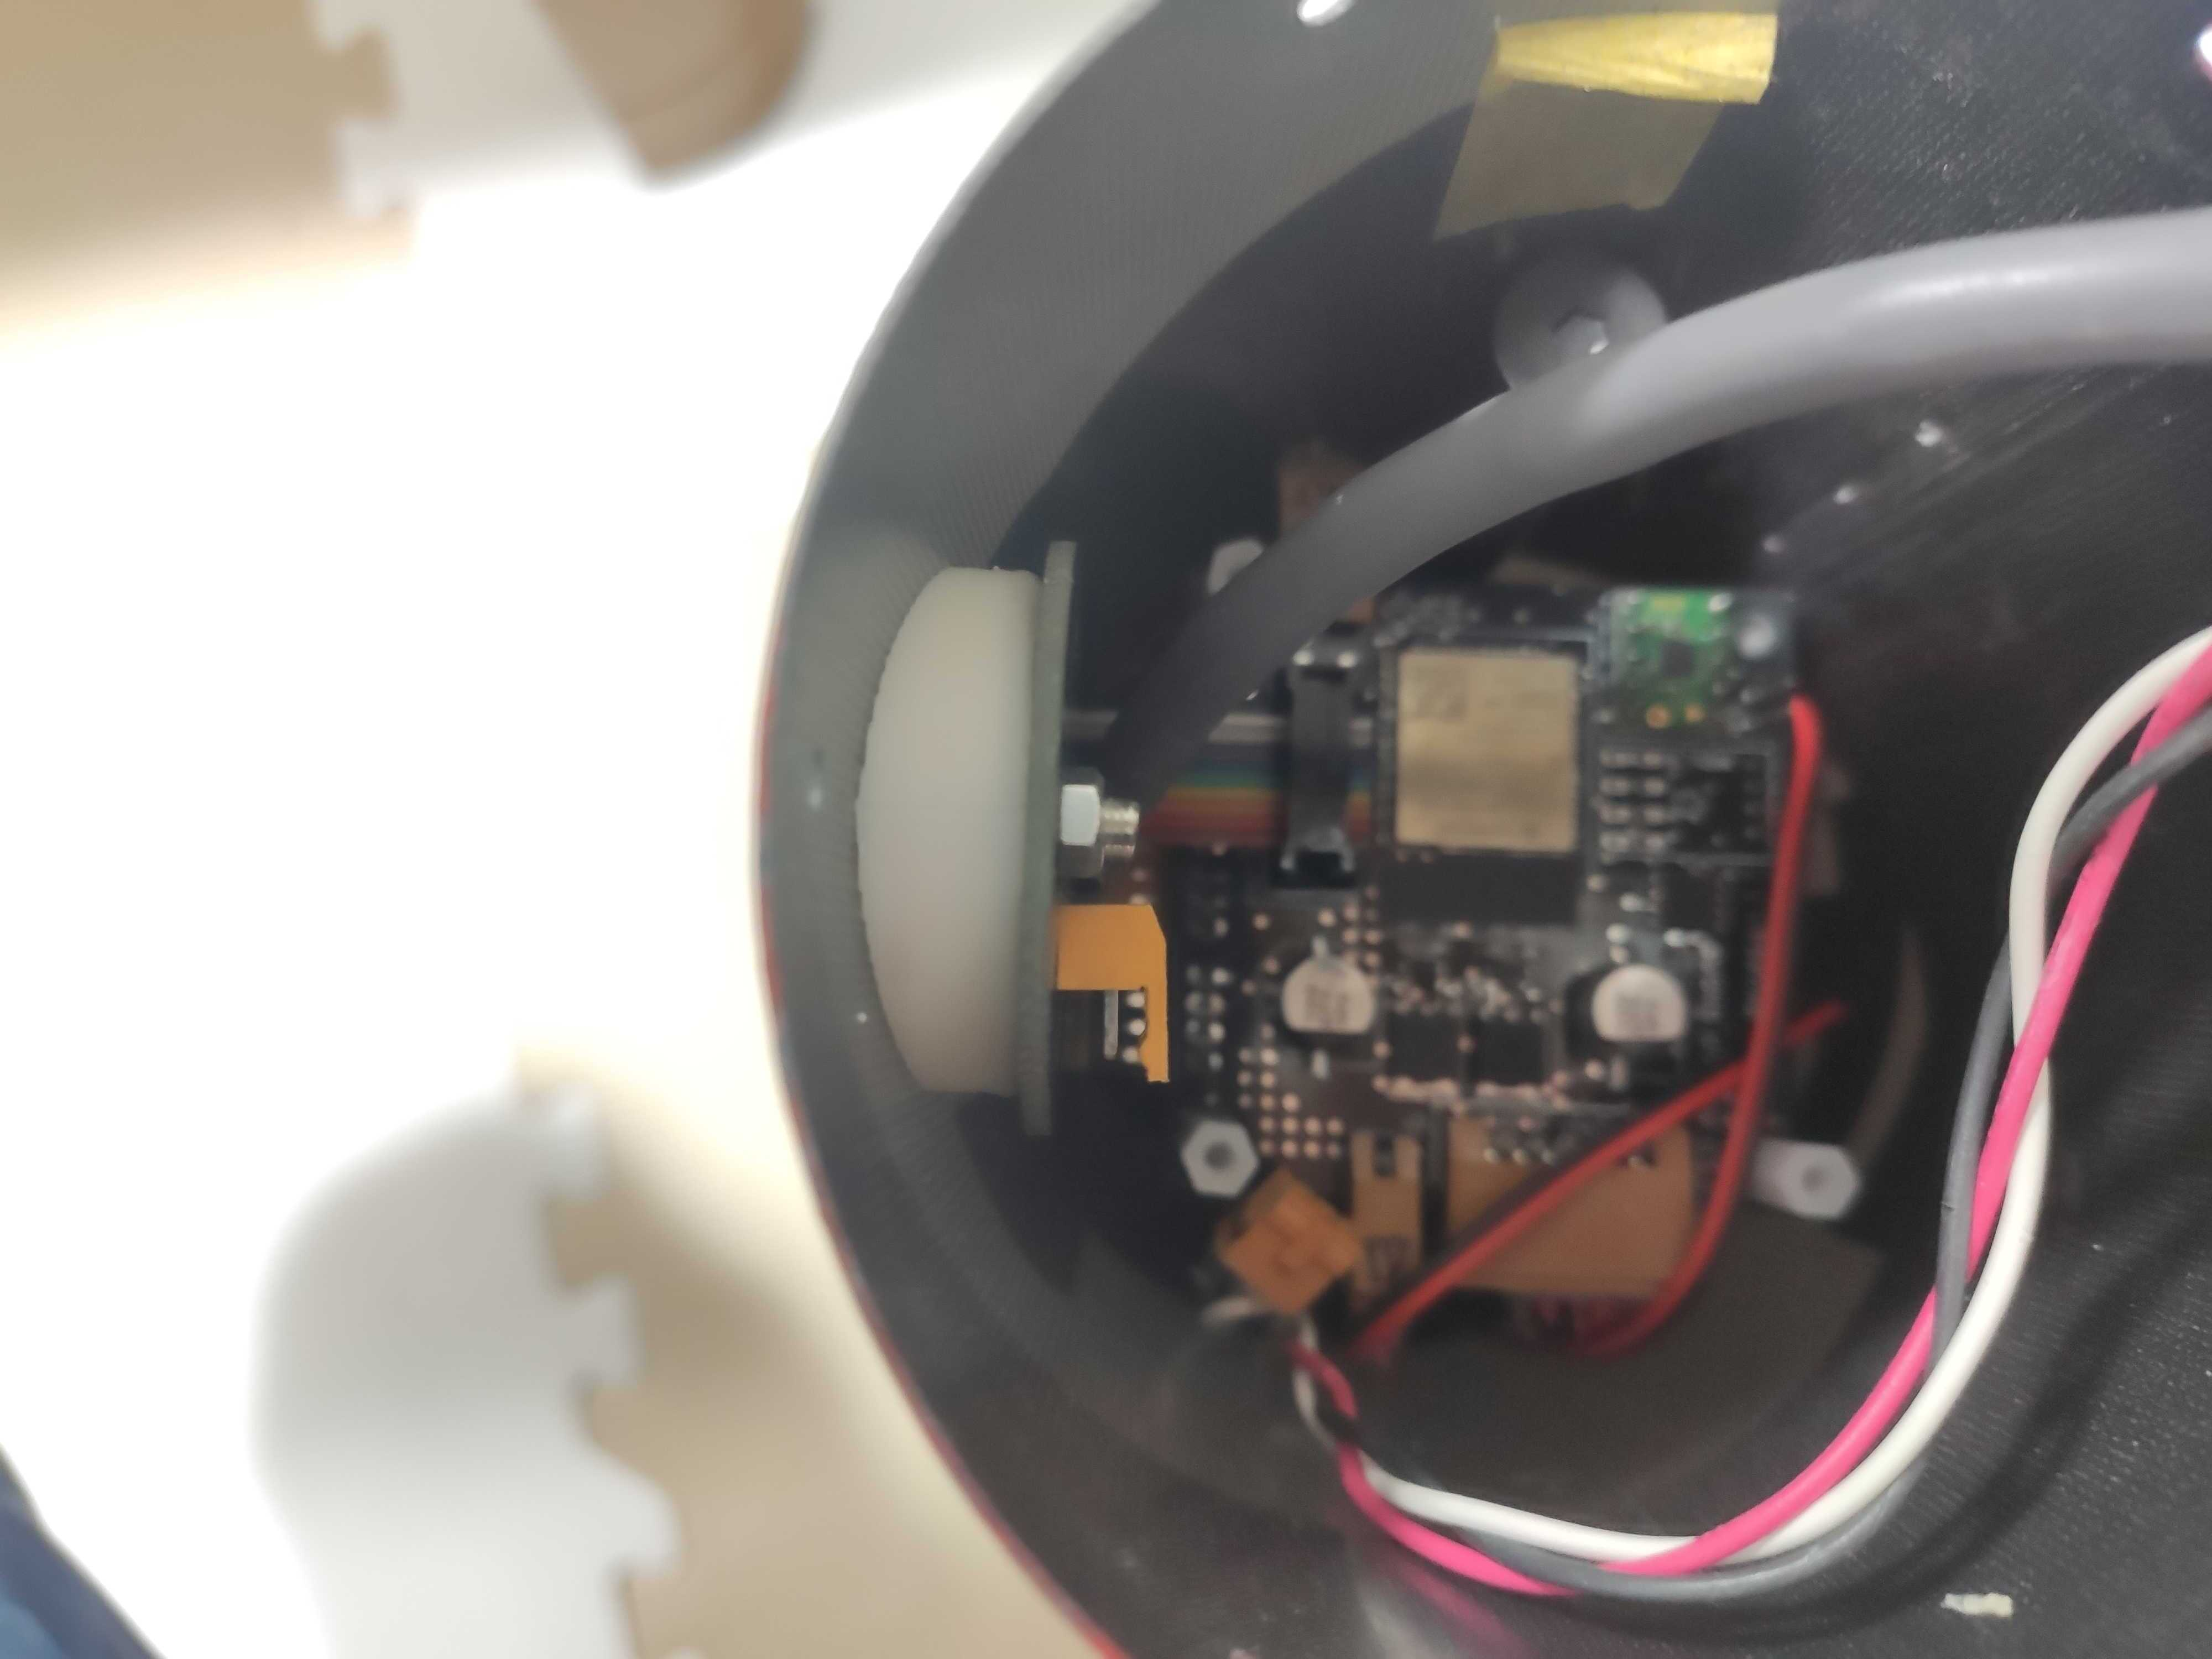
\includegraphics[scale = 0.05]{pic_avi/switch_in.jpg}
			\caption{スイッチ機構(内側)}\label{avi_switch_in}
		\end{minipage}
	\end{tabular}
\end{figure}

\section{データ解析・事後シミュレーション}
\label{sc:sim}
\subsection{位置・速度データ解析}
\label{itisokudo}
今回の打ち上げでは、開放基板及びミッション基板それぞれに搭載された6軸センサのロギング及びデータ取得に両者とも成功した。
取得した加速度・角速度センサの値を図\ref{fig:rokuziku}に示す。ただしミッション基板のデータは離床検知後30秒までのものであり、着地前にロギングを終了している。
また、角速度センサについては離床前のデータの平均値を取り、全体から減算する事により0点補正を行っている。
座標軸に関しては、射点を原点として磁東を基準としたENU座標系におけるものである。\footnote{x軸が磁東、y軸が磁北、z軸が鉛直上方向を示している。}


\begin{figure}[H]
	\begin{tabular}{cc}
		\begin{minipage}{.48\textwidth}
			\centering
			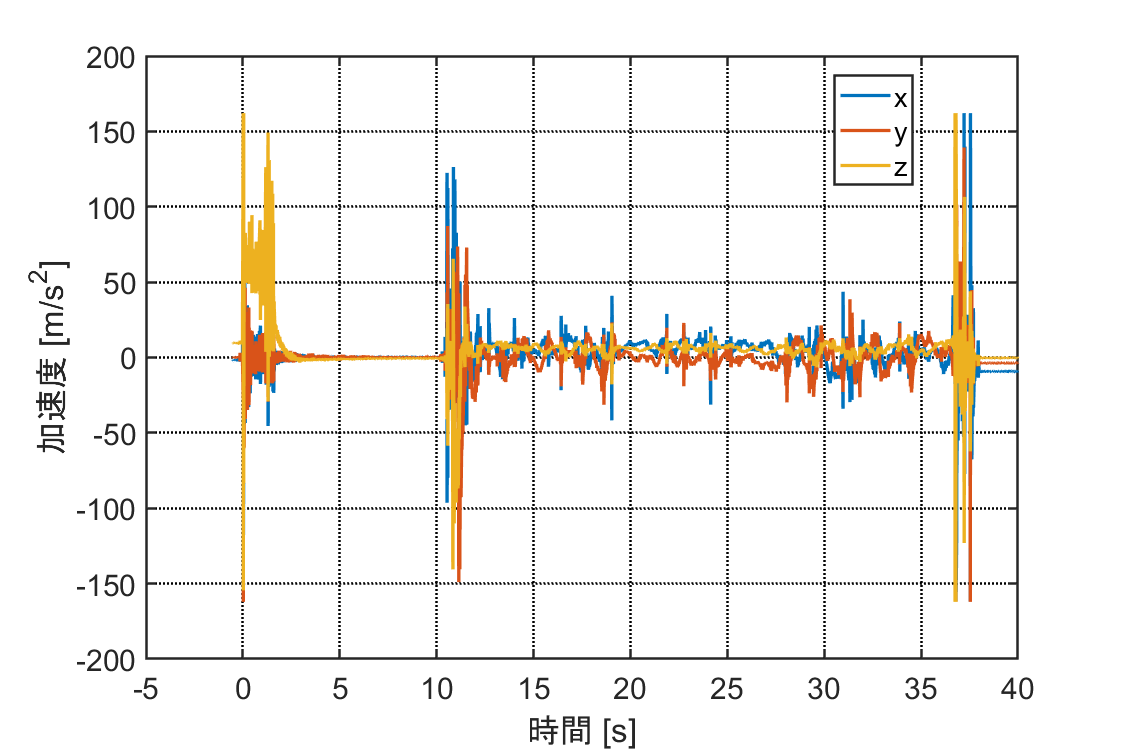
\includegraphics[width=75mm]{pic_sim/acc_no.png}
			\hspace{16mm} {\small[1]加速度データ(開放基板)}
		\end{minipage}
		\begin{minipage}{.48\textwidth}
			\centering
			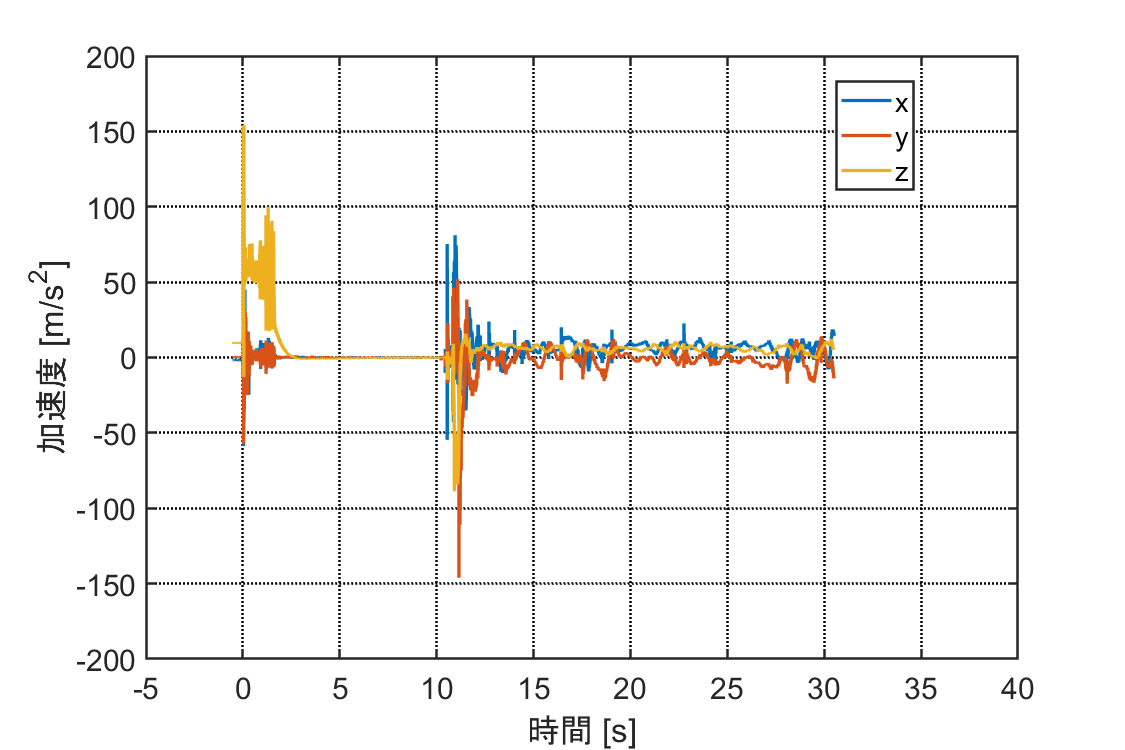
\includegraphics[width=75mm]{pic_sim/acc_ta.png}
			\hspace{16mm} {\small[2]加速度データ(ミッション基板)}
		\end{minipage}
	\end{tabular}
	\begin{tabular}{cc}
		\begin{minipage}{.48\textwidth}
			\centering
			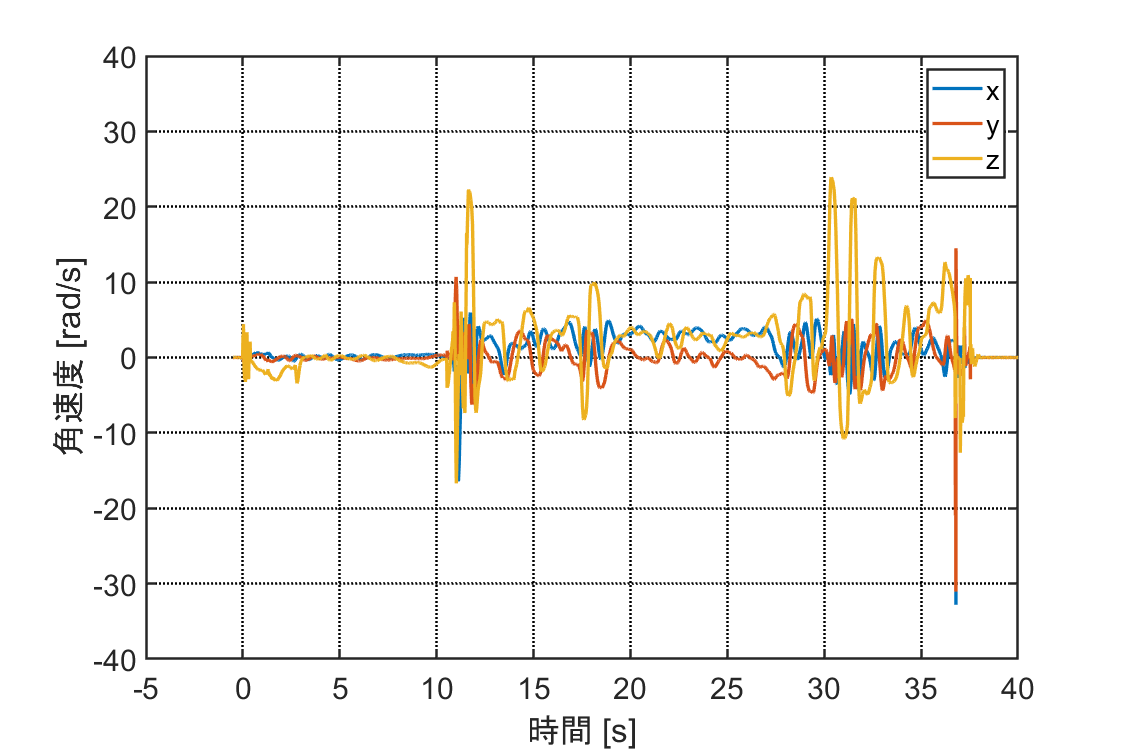
\includegraphics[width=75mm]{pic_sim/gyr_no.png}
			\hspace{16mm} {\small[3]角速度データ(開放基板)}
		\end{minipage}
		\begin{minipage}{.48\textwidth}
			\centering
			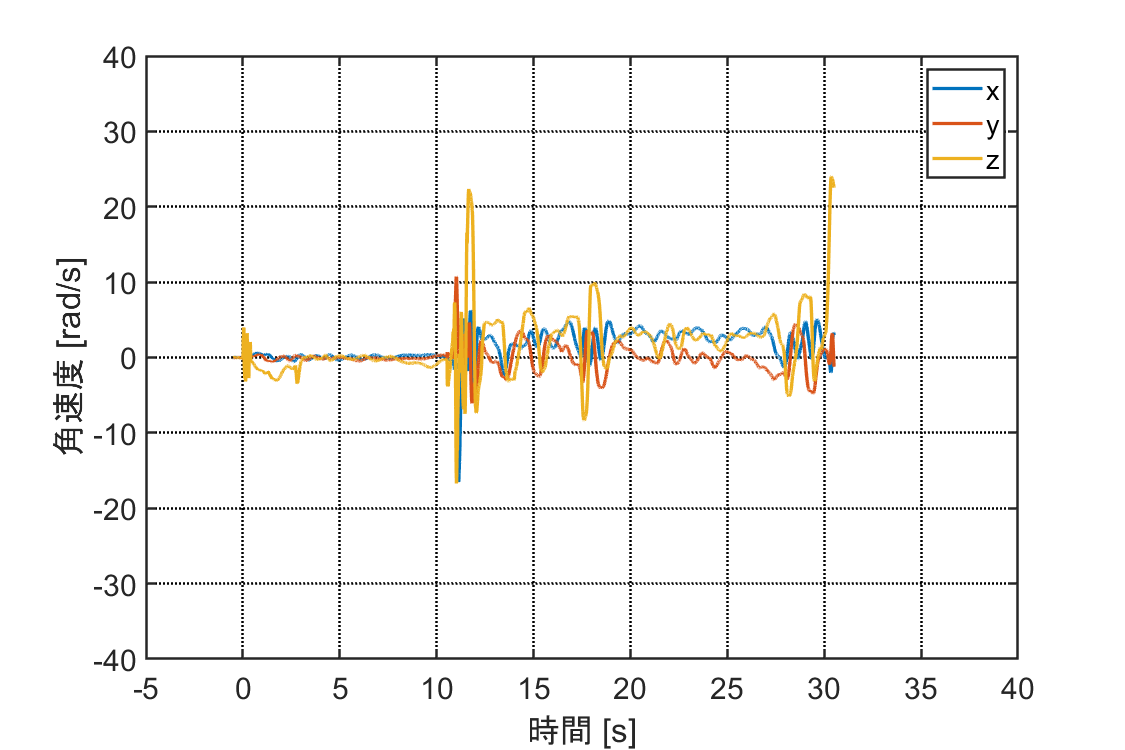
\includegraphics[width=75mm]{pic_sim/gyr_ta.png}
			\hspace{16mm} {\small[4]角速度データ(ミッション基板)}
		\end{minipage}
	\end{tabular}
	\caption{加速度・角速度センサデータ}
	\label{fig:rokuziku}
\end{figure}

取得した加速度・角速度データをもとに積分を行い、対地速度及び飛行経路を算出した。開放基板及びミッション基板それぞれの対地速度を図\ref{fig:taitisokudo}に、算出した飛行経路と実際の着地地点を図\ref{fig:hikoukeiro}に示す。
なお、パラシュート開傘以降の6軸センサの積分精度が悪くなることから、パラシュート開放以前は実線、以降は点線としてプロットしている。

\begin{figure}[H]
	\centering
	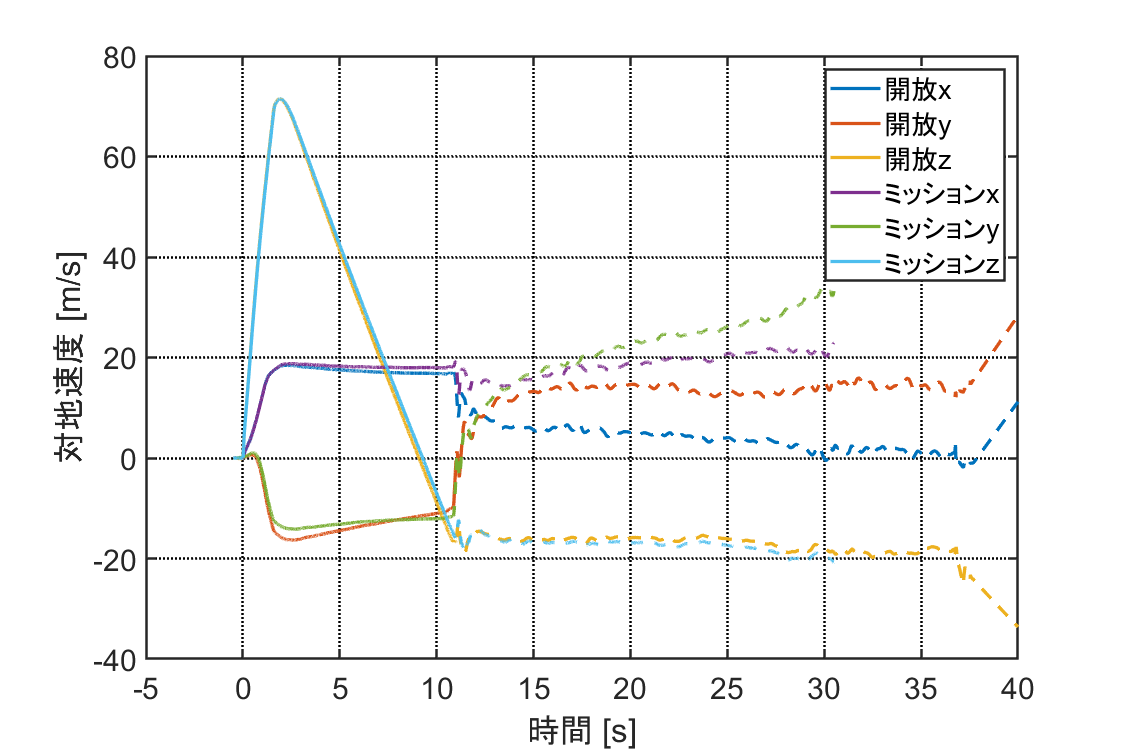
\includegraphics[width=0.7\linewidth]{pic_sim/Ve2.png}
	\caption{対地速度}
	\label{fig:taitisokudo}
\end{figure}

\begin{figure}[H]
	\begin{tabular}{cc}
		\begin{minipage}{.48\textwidth}
			\centering
			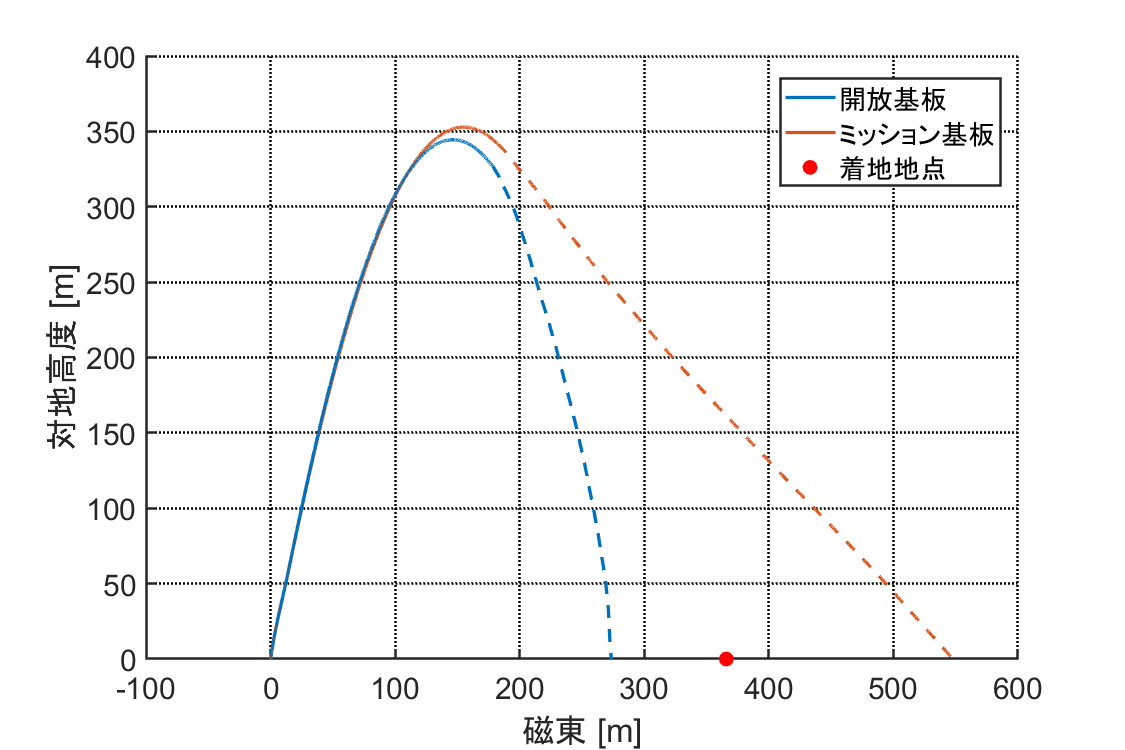
\includegraphics[width=75mm]{pic_sim/pos2_eh.png}
			\hspace{16mm} {\small[1]磁東-対地高度}
		\end{minipage}
		\begin{minipage}{.48\textwidth}
			\centering
			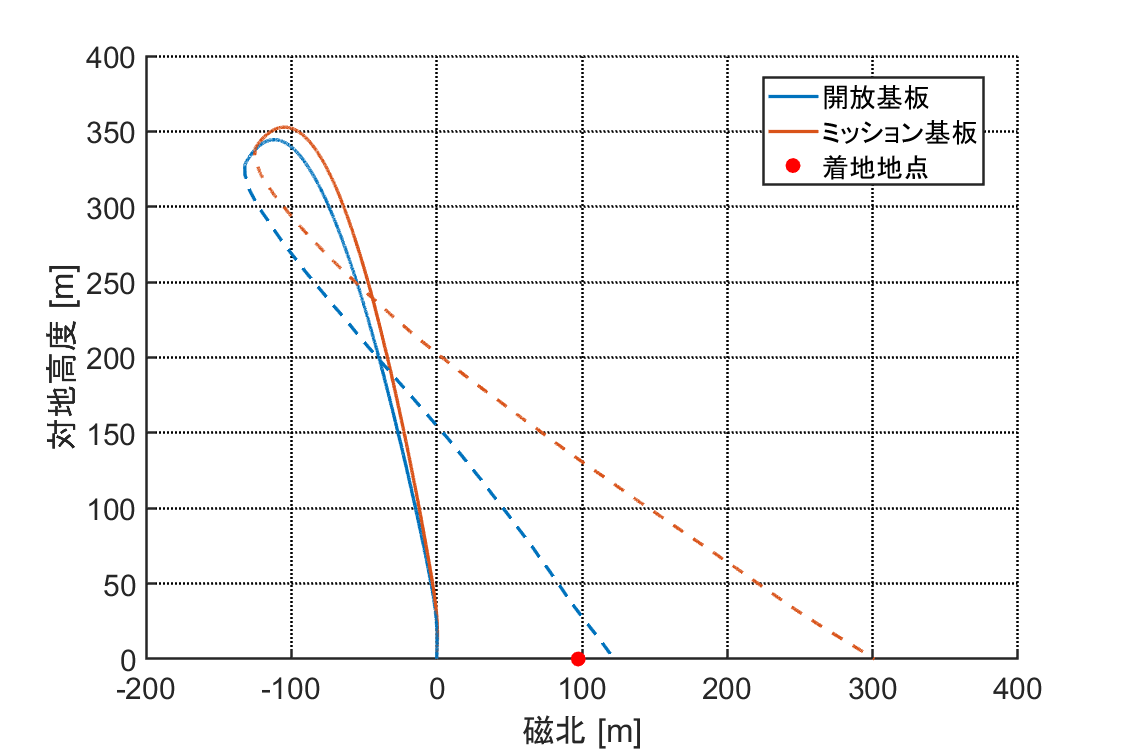
\includegraphics[width=75mm]{pic_sim/pos2_nh.png}
			\hspace{16mm} {\small[2]磁北-対地高度}
		\end{minipage}
	\end{tabular}
	\centering
	\begin{minipage}{.48\textwidth}
		\centering
		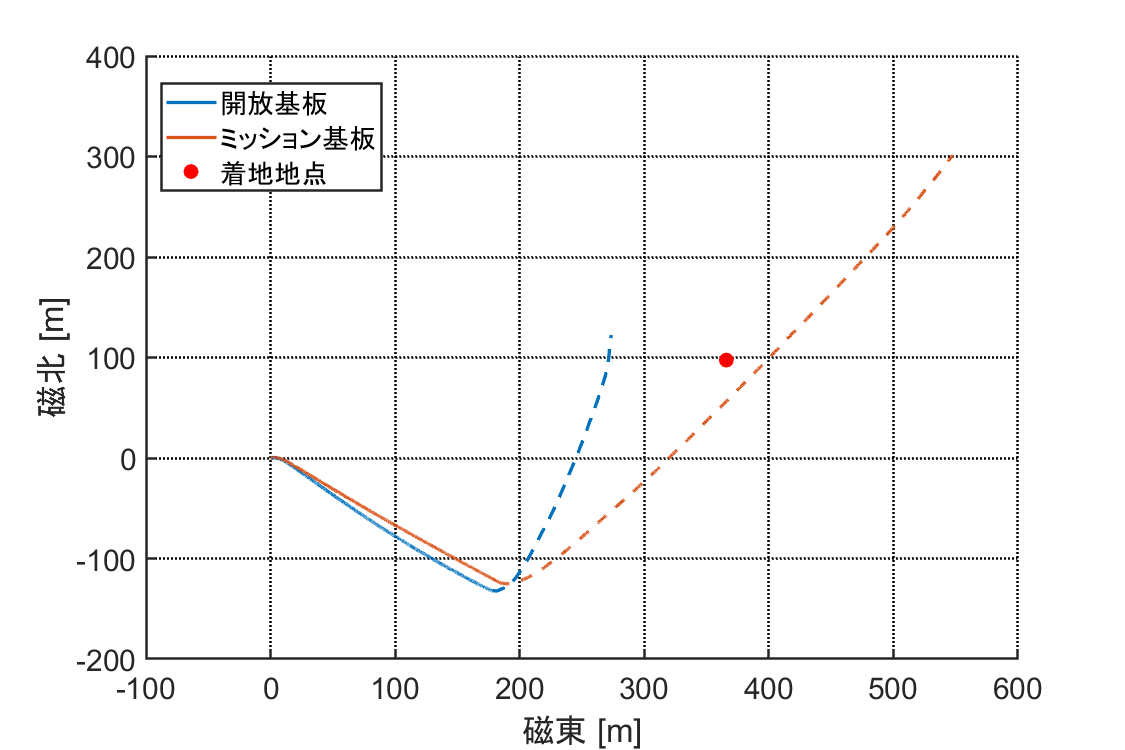
\includegraphics[width=75mm]{pic_sim/pos2_en.png}
		\hspace{16mm}{\small[3]磁東-磁北}
	\end{minipage}
	\caption{飛行経路}
	\label{fig:hikoukeiro}
\end{figure}

\begin{table}[H]
	\centering
	\caption{頂点座標}
	\label{tab:tyouten_kiban}
	\begin{tabular}{cccc}
		\hline
		      & x (\si{m}) & y (\si{m}) & z (\si{m}) \\\hline
		開放    & 146.2      & $-111.8$   & 344.5      \\
		ミッション & 155.1      & $-104.7$   & 352.8      \\
		\hline
	\end{tabular}
\end{table}

\begin{table}[H]
	\centering
	\caption{ランチクリア速度}
	\label{tab:launch_sokudo}
	\begin{tabular}{ccc}
		\hline
		      & 時刻 (\si{s}) & ランチクリア速度 (\si{m/s}) \\
		\hline
		開放    & 0.42        & 23.2                \\
		ミッション & 0.42        & 22.7                \\
		\hline
	\end{tabular}
\end{table}

ここで、取得した加速度を地上座標系における機体の重心での値への変換式は式\eqref{eq:kasokudohennkann}に、各変数については表\ref{tab:henkan_keisu}に示す。

\begin{equation}
	\bm{a}_e = C_{e/b}\left(\bm{a}_s-\bm{\omega}\times \bm{\omega}\times \bm{X}_s\right)-\bm{g}_e
	\label{eq:kasokudohennkann}
\end{equation}

\begin{table}[H]
	\centering
	\caption{式\eqref{eq:kasokudohennkann}諸元}
	\label{tab:henkan_keisu}
	\begin{tabular}{lccr}
		\toprule
		\multicolumn{1}{c}{名称} & 変数            & 単位           \\
		\midrule
		加速度ベクトル(センサ値)          & $\bm{e}_s$    & \SI{}{m/s^2} \\
		加速度ベクトル(地上座標系)         & $\bm{e}_e$    & \SI{}{m/s^2} \\
		角速度(機体座標系)             & $\bm{\omega}$ & \SI{}{rad/s} \\
		座標変換行列                 & $C_{e/b}$     & -            \\
		センサ位置                  & $\bm{X}_s$    & $\SI{}{m}$   \\
		重力(地上座標系)              & $\bm{g}_e$    & \SI{}{m/s^2} \\
		\bottomrule
	\end{tabular}
\end{table}


図\ref{fig:taitisokudo}と図\ref{fig:hikoukeiro}からわかるように、2つのデータは頂点到達までは、対気速度及び飛行経路ともに大方一致していることがわかる。
頂点到達時の座標は表\ref{tab:tyouten_kiban}に示しているように、その差は直線距離にして\SI{14}{m}である。
独立した2つのセンサから同様の経路を算出できたことから、頂点到達前に関しては実際の対地速度及び飛行経路と近いものが得られたと考えられる。

一方で頂点到達以降に関しては、2つの算出結果に大きな差が生じていることがわかる。
これはパラシュート開傘時の運動がサンプリングレートより高い周波数の運動であることが原因と考えられる。
すなわち、6軸センサではパラシュート開傘後の運動を十分に追跡できなかったため、2つのセンサ間の差が拡大したと考えられる。

\subsection{高度データ解析}
\label{koudo}
離床時刻からの機体の高度は気圧センサのデータからも算出可能である。図\ref{fig:koudozikannkeika}に気圧センサ及び\ref{itisokudo}項で算出した高度の時間経過を、表にそれぞれの頂点到達時間及び最高到達高度を示す。

\begin{figure}[H]
	\centering
	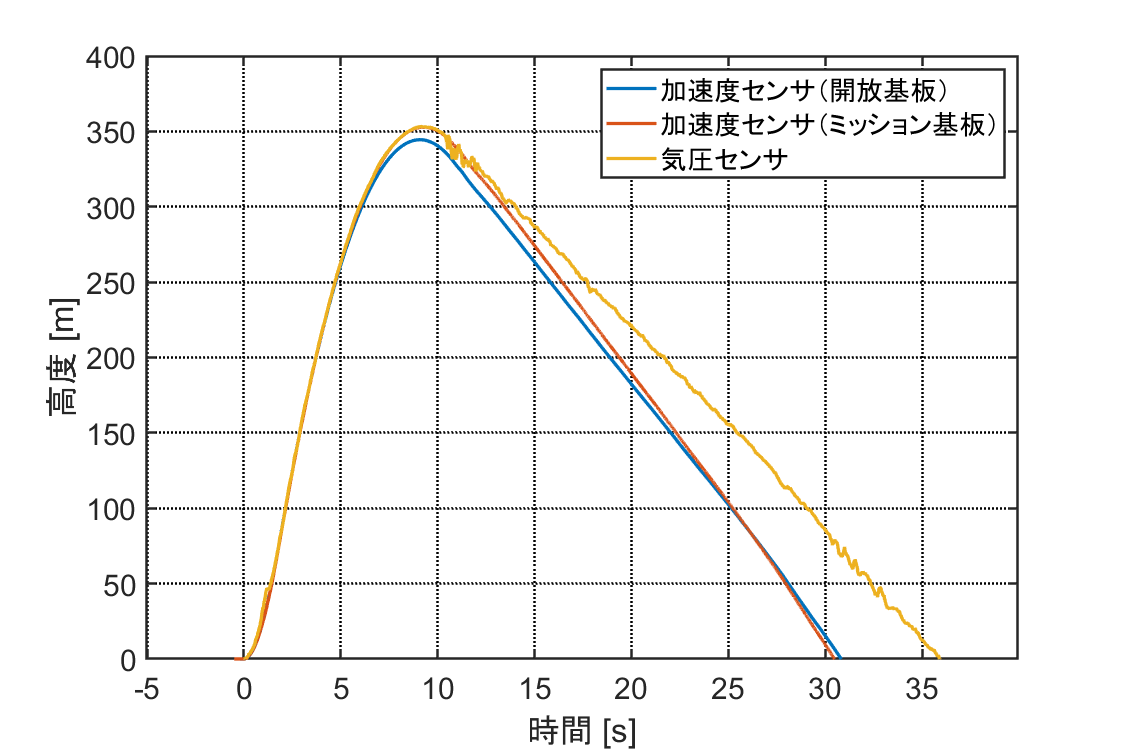
\includegraphics[width=0.7\linewidth]{pic_sim/pos_h.png}
	\caption{高度の時間経過}
	\label{fig:koudozikannkeika}
\end{figure}

\begin{table}[H]
	\centering
	\caption{頂点到達時間及び最高到達高度}
	\label{tab:tyouten}
	\begin{tabular}{ccc}
		\hline
		      & 頂点到達時間 (\si{s}) & 高度 (\si{m}) \\\hline
		開放    & 9.08            & 344.5       \\
		ミッション & 9.27            & 352.8       \\
		気圧センサ & 9.48            & 353.0       \\
		\hline
	\end{tabular}
\end{table}

\begin{figure}[H]
	\centering
	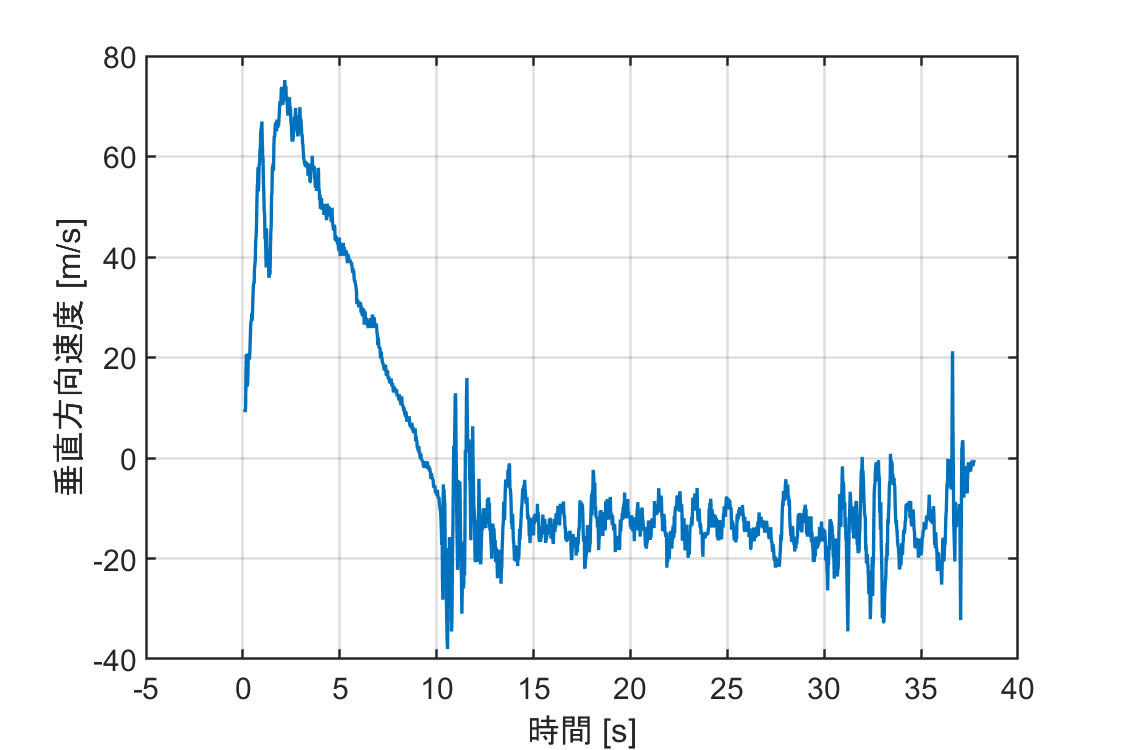
\includegraphics[width=0.7\linewidth]{pic_sim/hight_d.png}
	\caption{気圧センサから算出した垂直方向速度}
	\label{fig:suityoku_kiatu}
\end{figure}

図\ref{fig:suityoku_kiatu}は気圧センサから取得した高度を微分したものである。
ただし、変化を明瞭にするため0.4秒間、データ数にして20個のデータで移動平均を出したものをプロットしている。
パラシュート開傘時刻が離床から10.2秒後であり、比較的降下速度が安定しているのが\SI{12.5}{s}付近であることから、
開傘から終端速度到達までに\SI{2.5}{s}ほどかかっていることがうかがえる。
終端速度に関しては、\SI{15.0}{s}から\SI{30.0}{s}の間に\SI{274.3}{m}降下していることから、終端速度は\SI{13.2}{m/s}であることがわかった。
表\ref{tab:kouryoku_shogen}に記載する諸元を用いて計算した結果、パラシュートの抗力係数は1.27であることがわかった。

\begin{table}[H]
	\centering
	\caption{抗力係数算出諸元}
	\label{tab:kouryoku_shogen}
	\begin{tabular}{lcr}
		\toprule
		\multicolumn{1}{c}{諸元名} & 単位          & \multicolumn{1}{c}{値} \\
		\midrule
		降下速度                    & \si{m/s}    & 13.71                 \\
		燃焼終了後重量                 & \si{kg}     & 5.894                 \\
		気体密度                    & \si{kg/m^3} & 1.144                 \\
		代表面積                    & \si{m^3}    & 0.422                 \\
		\midrule
		抗力係数                    & -           & 1.27                  \\
		\bottomrule
	\end{tabular}
\end{table}

\subsection{姿勢データ解析}
取得した角速度データから、飛行中の機体の姿勢を表すクォータニオンを算出した。図\ref{fig:quatarnionhikaku}にそれぞれの基板のから算出した値を示す。
またこれらクォータニオンを動翼の制御に使用したyxzオイラー角に変更したものを図\ref{fig:oirahikaku}に示す。

\begin{figure}[H]
	\centering
	\begin{minipage}{.85\textwidth}
		\centering
		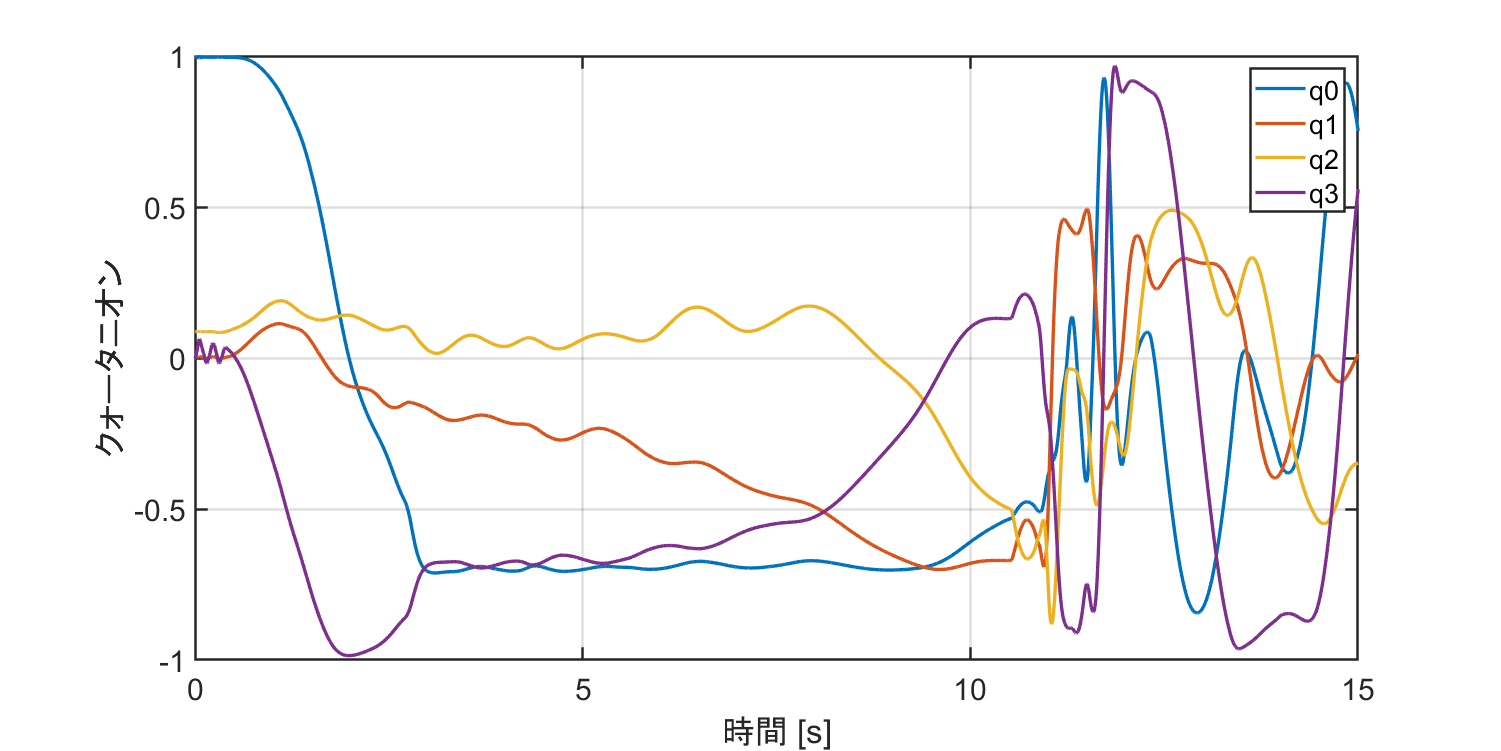
\includegraphics[width=0.95\linewidth]{pic_sim/qua_no_s.png}
		\hspace{16mm}{\small[1]開放基板}

		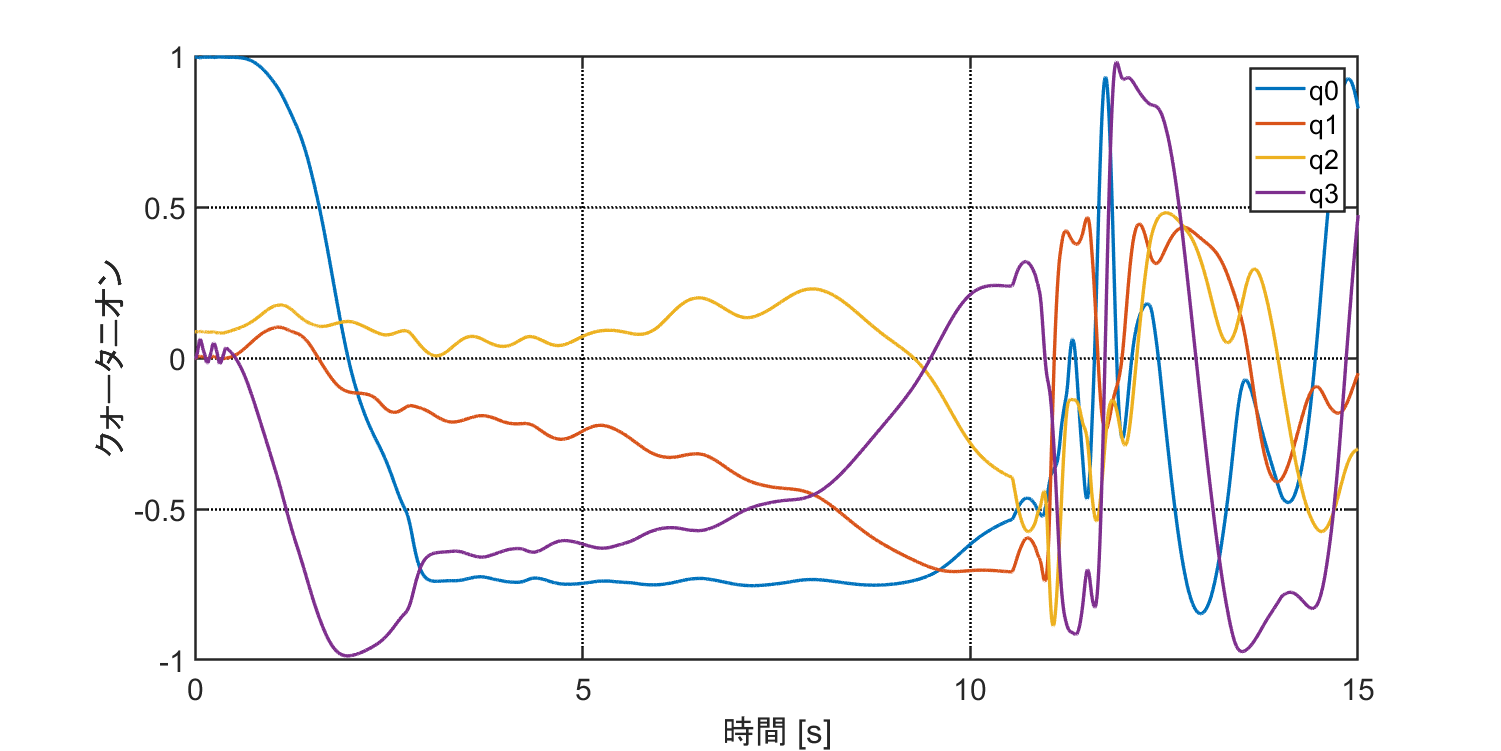
\includegraphics[width=0.95\linewidth]{pic_sim/qua_ta_s.png}
		\hspace{16mm}{\small[2]ミッション基板}
	\end{minipage}
	\caption{算出したクォータニオン}
	\label{fig:quatarnionhikaku}
\end{figure}

\begin{figure}[H]
	\centering
	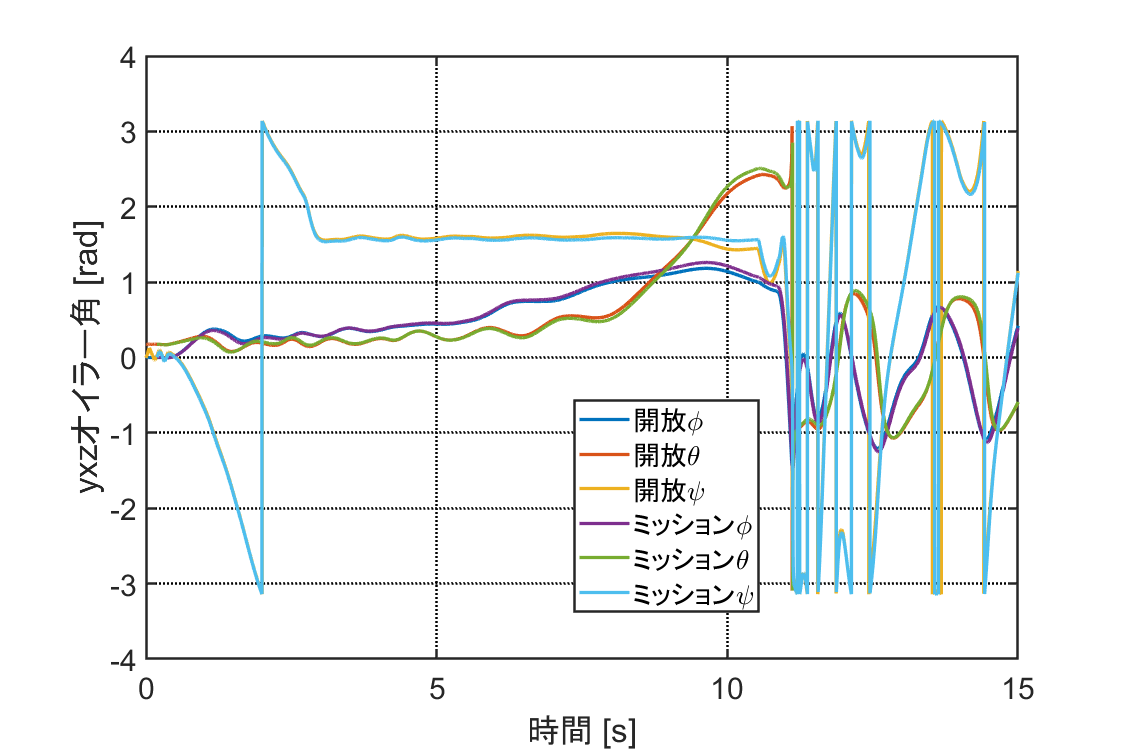
\includegraphics[width=0.65\linewidth]{pic_sim/euler2.png}
	\caption{yxzオイラー角の比較}
	\label{fig:oirahikaku}
\end{figure}

\begin{figure}[H]
	\begin{tabular}{cc}
		\begin{minipage}{.48\textwidth}
			\centering
			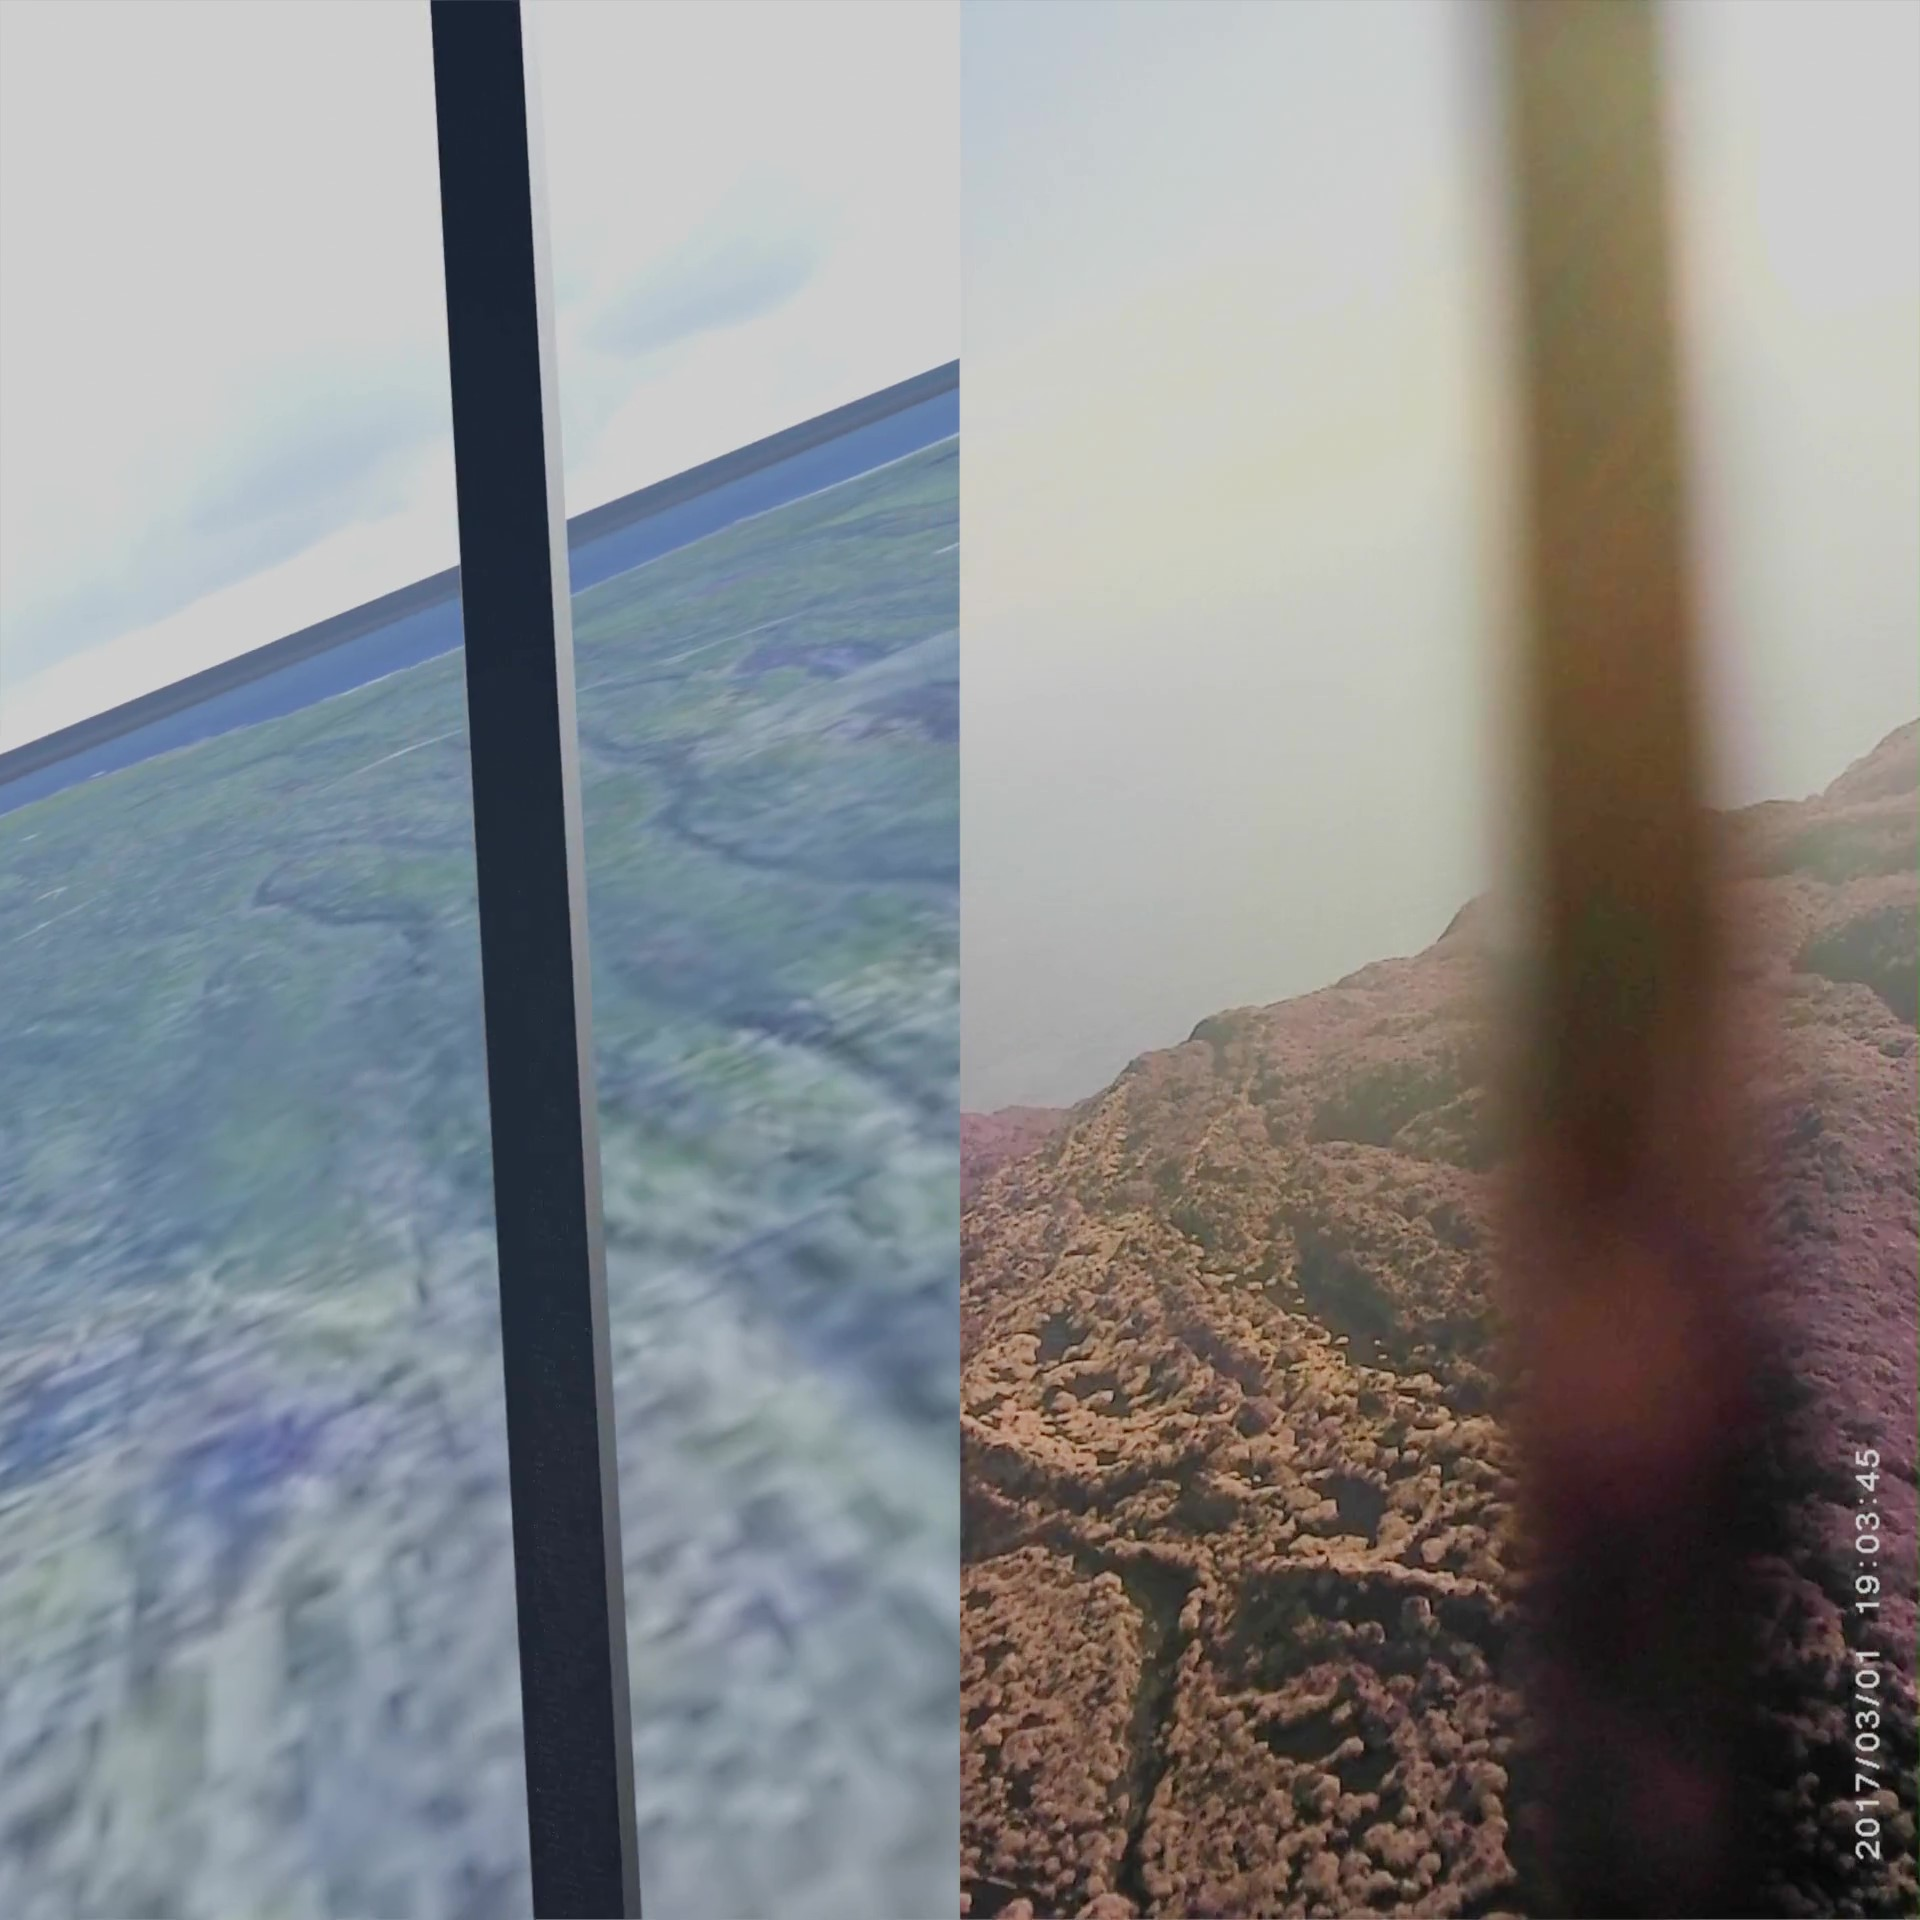
\includegraphics[width=75mm]{pic_sim/compare_5.jpg}
			\hspace{16mm} {\small[1] 離床5秒後(左:CG、右:機体カメラ)}
		\end{minipage}
		\begin{minipage}{.48\textwidth}
			\centering
			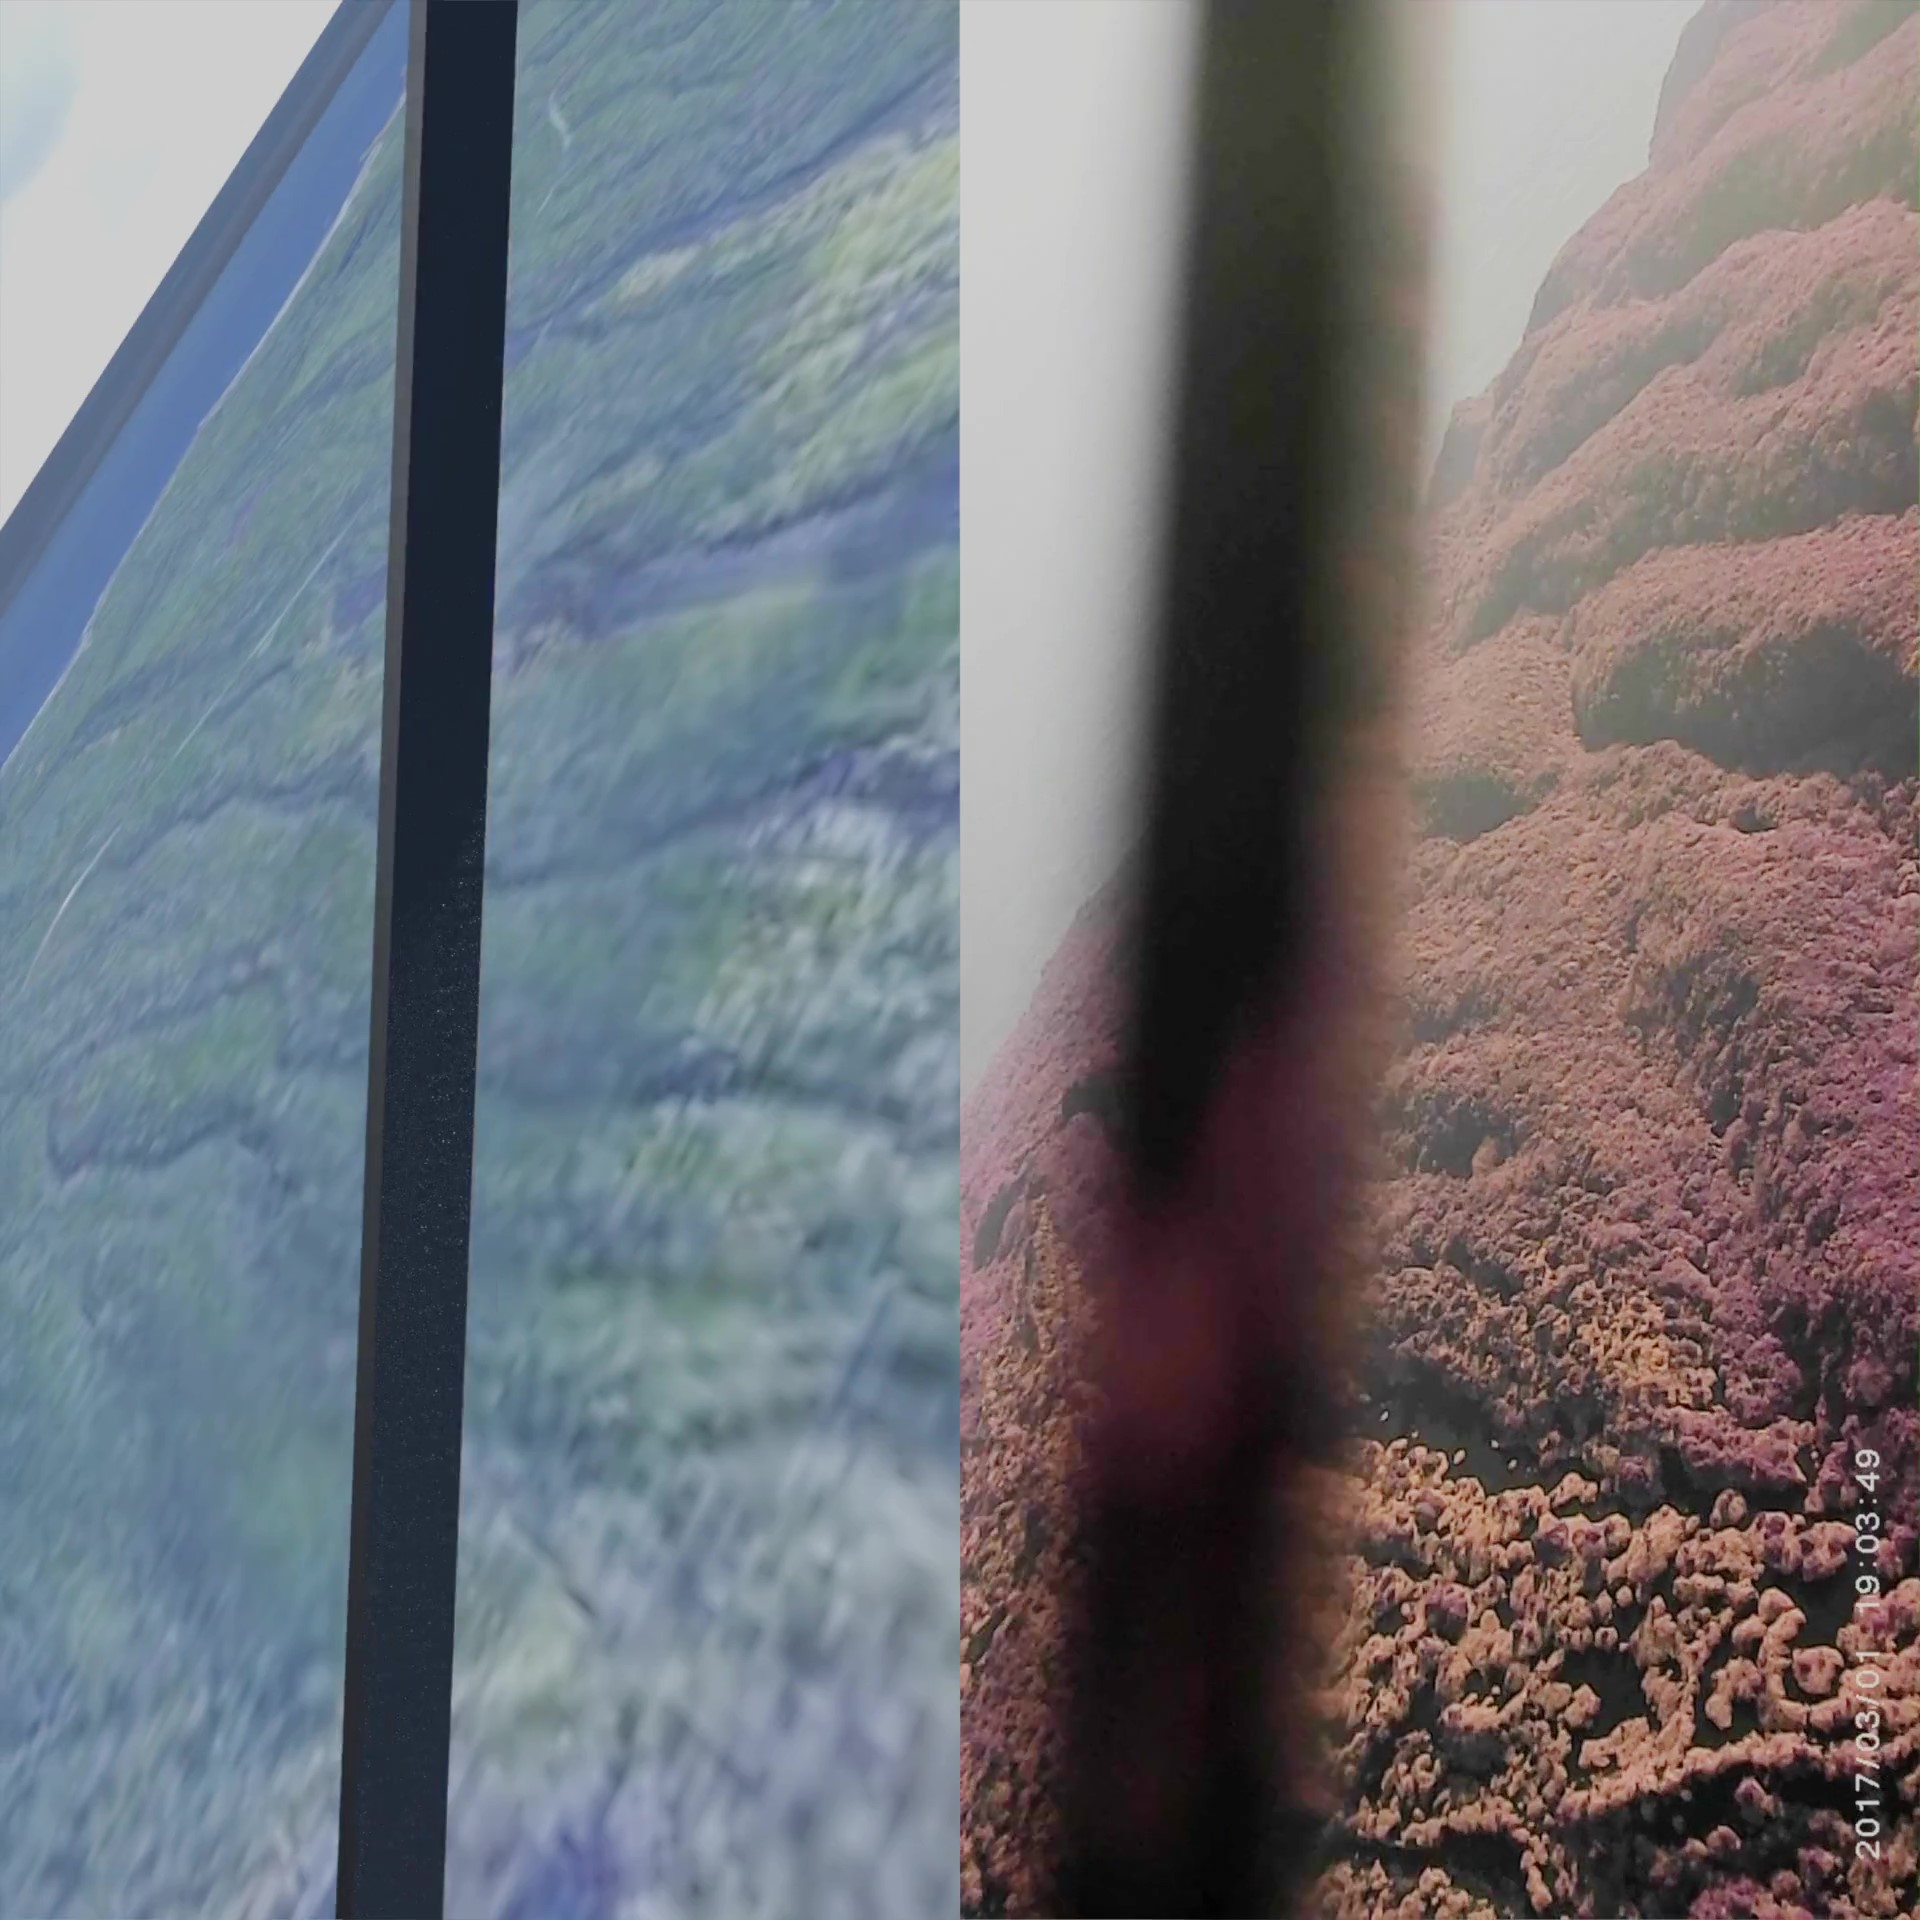
\includegraphics[width=75mm]{pic_sim/compare_8.jpg}
			\hspace{16mm} {\small[2] 離床8秒後(左:CG、右:機体カメラ)}
		\end{minipage}
	\end{tabular}
	\centering
	\caption{CGと機体カメラの映像の比較}
	\label{fig:dougahikaku}
\end{figure}

図\ref{fig:oirahikaku}に示した通り、それぞれの基板のセンサから算出した姿勢にほとんど差異は見られなかった。パラシュート開傘以前において、その差の最大値は$\psi$で\SI{6.9}{deg}であった。
図\ref{fig:dougahikaku}に示しているように、機体に搭載したカメラからの動画映像と、算出したクォーターニオンの値を用いて作成したCG映像を比較しても、その差がほとんど見られないことが確認できた。

次に、取得した磁気センサの値の精度を評価する。
磁気センサの零点補正を行うため、最小二乗法を用いて球面フィッテングを行った。補正した結果を図\ref{fig:tiziki}に、ノルムの時間変化を図\ref{fig:tizikinorumu}に示す。


\begin{figure}[H]
	\centering
	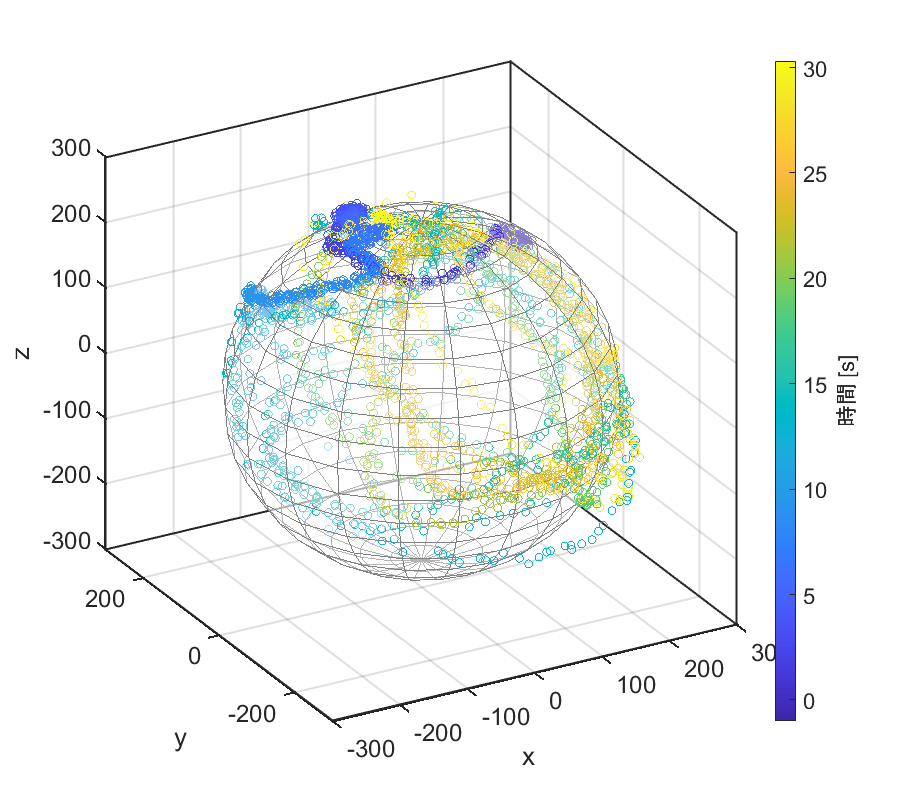
\includegraphics[width=0.7\linewidth]{pic_sim/mag_fix.png}
	\caption{零点補正後の磁気センサ}
	\label{fig:tiziki}
\end{figure}
\begin{figure}[H]
	\centering
	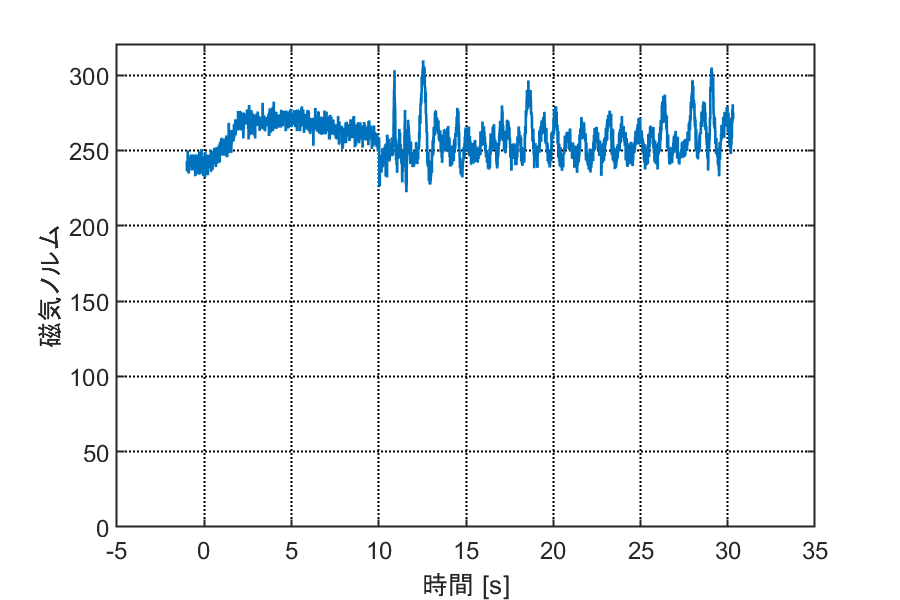
\includegraphics[width=0.7\linewidth]{pic_sim/mag_norm.png}
	\caption{零点補正後の磁気センサノルム}
	\label{fig:tizikinorumu}
\end{figure}

ここで算出したクォーターニオンを用いて磁気センサの値を地上座標系に変換したものを図\ref{fig:tizikihennkann}に示す。

\begin{figure}[H]
	\centering
	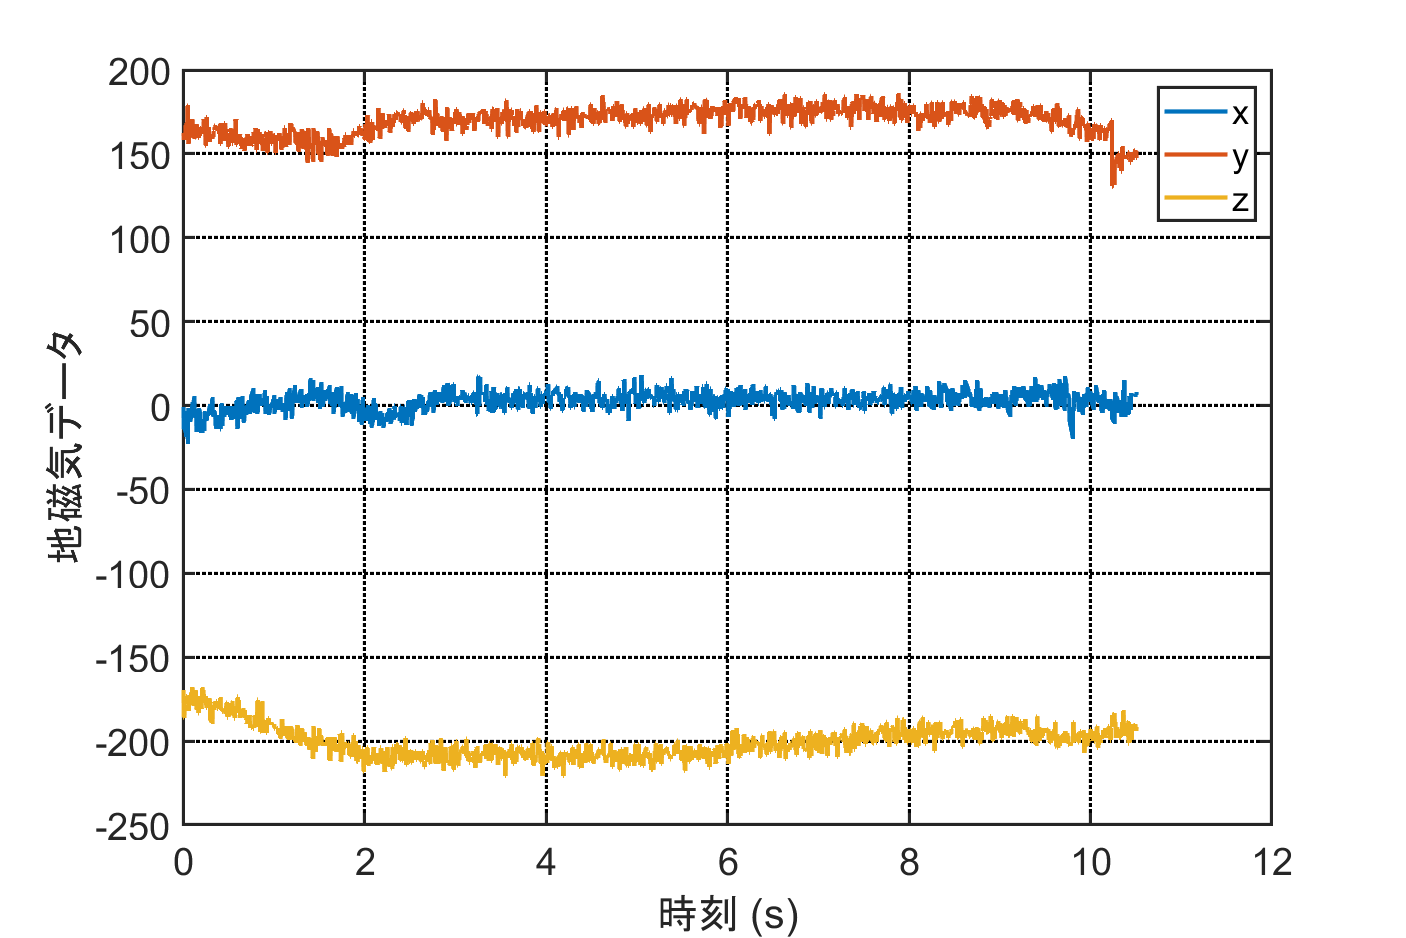
\includegraphics[width=0.7\linewidth]{pic_sim/mag_tijou.png}
	\caption{磁気ベクトルの各成分(地上座標系)}
	\label{fig:tizikihennkann}
\end{figure}

射点付近の地磁気ベクトルは定ベクトルであるとみなせるため、図\ref{fig:tizikihennkann}に示した磁気センサのENU座標系での各軸の値が一定なっていることがわかる。
また、磁東方向の値が$0$、磁北方向が正の値、鉛直方向が負の値(鉛直下向き)になっていることから、地磁気の向きと整合性があることもわかる。\footnote{地磁気は俯角を持つため、地磁気ベクトルは鉛直下向き成分を持つ。}
さらに、図\ref{fig:tizikinorumu}と図\ref{fig:tizikihennkann}からわかるように、およそ\SI{10.2}{s}以降から磁気センサのノルムやy方向の値が乱れている。
これは動翼制御用モータが発生させる磁場の影響であると考えられる。
以上より、パラシュート開傘以前の磁気センサの値は十分な精度で地磁気の値を取得していることがわかる。そのため、算出したクォータニオンのデータの正確性も担保された。

\subsection{動翼データ解析}
\label{sc:data_doyoku}
ここでは、ミッション基板のデータをもとにロール制御の精度を評価する。図\ref{fig:ロール角}に離床から制御終了までのロール角の時間変化を示す。
離床から制御開始までを青色、制御開始から制御終了までを赤色で示し、目標ロール角\SI{90}{deg}を黒色で示した。離床約2.71秒後に制御を開始し、その後0.3秒間程度で目標ロール角付近に収束していることがわかる。
目標ロール角付近に収束した離床約\SI{3}{s}から制御終了までの二乗平均平方根誤差は約\SI{1.98}{deg}であり、高い精度で制御できたことがわかる。誤差の原因は、外乱ロールモーメントや動翼機構のバックラッシの影響が考えられる。\par
\begin{figure}[H]
	\centering
	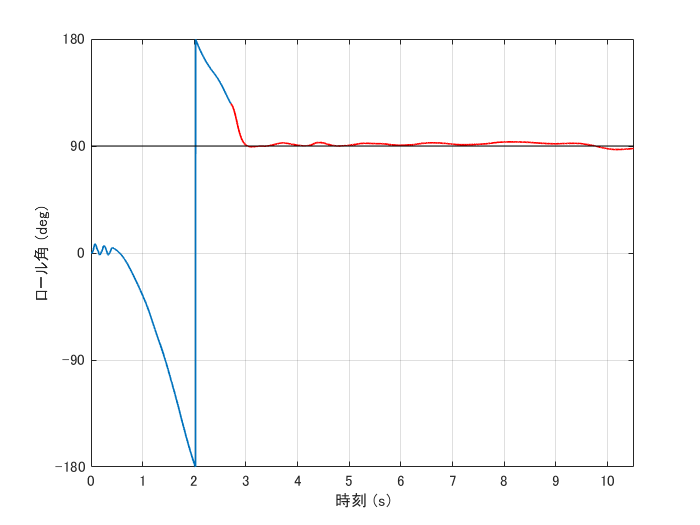
\includegraphics[width=0.8\linewidth]{pic_avi/ロール角.png}
	\caption{ロール角の時間変化}
	\label{fig:ロール角}
\end{figure}
図\ref{fig:動翼角度}に離床から制御終了までの動翼角度の時間変化を青色で示す。また、目標動翼角度の時間変化を黒色で示す。
動翼角度が目標値に高い精度で追従していることがわかる。図\ref{fig:動翼角度_切り取り}に離床後\SI{2.70}{s}から\SI{2.90}{s}までを抜き出したグラフを示す。
動翼角度が目標値にわずかに遅れて追従していることがわかる。離床後約\SI{2.76}{s}から約\SI{2.79}{s}までの間、目標値が\SI{-15}{deg}で一定値なのに対して動翼角度が約\SI{14.74}{deg}で停止しており、誤差がある。
これは、空力により動翼の軸まわりにはたらくモーメントの影響だと考えられる。
エンジン燃焼終了から間もないため対気速度が大きく、動翼角度の絶対値も大きいため、モーメントが大きい状況であり、誤差が大きくなったと考えられる。
\begin{figure}[H]
	\centering
	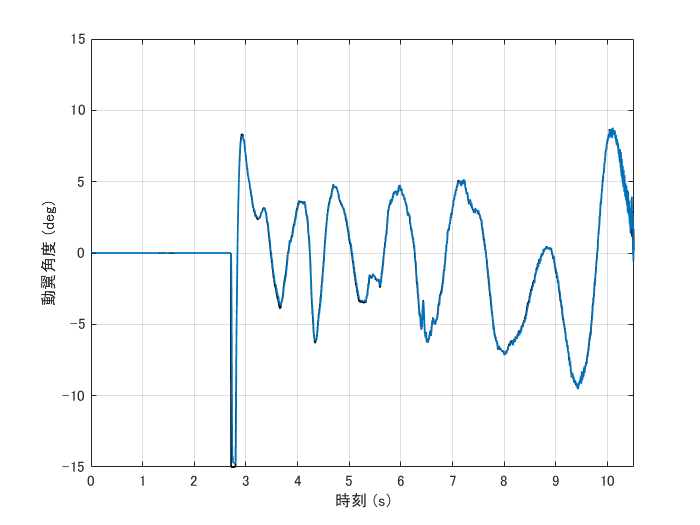
\includegraphics[width=0.8\linewidth]{pic_avi/動翼角度.png}
	\caption{動翼角度と目標動翼角度の時間変化}
	\label{fig:動翼角度}
\end{figure}
\begin{figure}[H]
	\centering
	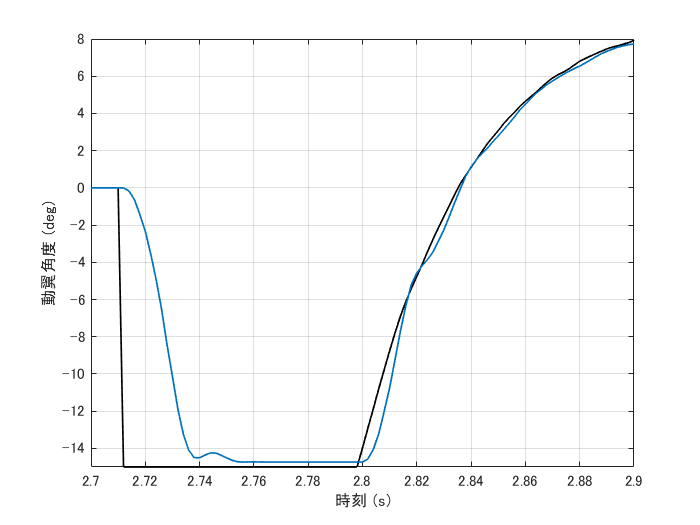
\includegraphics[width=0.8\linewidth]{pic_avi/動翼角度_切り取り.png}
	\caption{離床後\SI{2.7}{s}から\SI{2.9}{s}までの動翼角度と目標動翼角度の時間変化}
	\label{fig:動翼角度_切り取り}
\end{figure}


\subsection{推力履歴について}
\label{suiryokurireki}
加速度データから打ち上げ時のエンジンの推力履歴を算出した。開放基板、ミッション基板から算出したものと、直近の2022年7月に実施された燃焼試験での値を図\ref{fig:suiryokurireki}に示す。
また推力に関する各諸元を表\ref{tab:nenshoushogen}に、加速度データから推力の算出式を式\eqref{eq:T}に、各変数を表\ref{tab:eqshogen}に示す。

\begin{figure}[H]
	\centering
	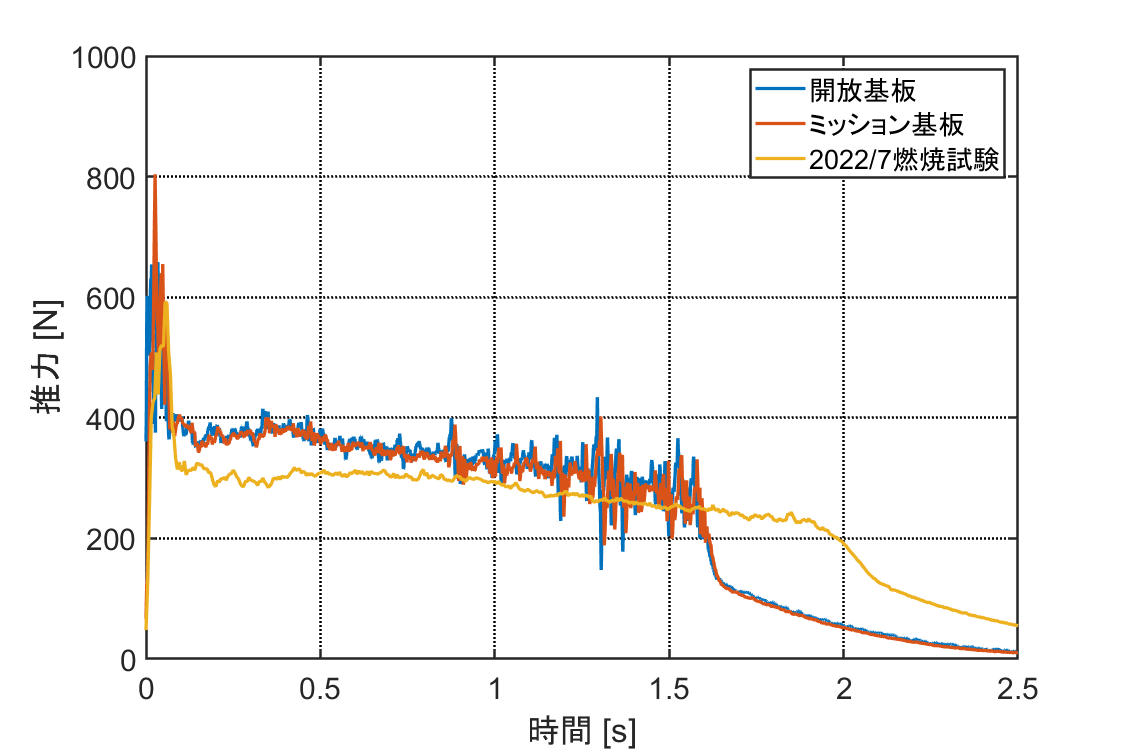
\includegraphics[width=0.7\linewidth]{pic_sim/acc_thrust.png}
	\caption{推力履歴の比較}
	\label{fig:suiryokurireki}
\end{figure}

\begin{table}[H]
	\centering
	\caption{燃焼諸元}
	\label{tab:nenshoushogen}
	\begin{tabular}{lcrrr}
		\hline
		名称        & 単位         & \multicolumn{1}{c}{開放} & \multicolumn{1}{c}{ミッション} & \multicolumn{1}{c}{7月燃焼試験} \\
		\hline
		トータルインパルス & \SI{}{N.s} & 596                    & 581                       & 628                        \\
		平均推力      & \SI{}{N}   & 273                    & 280                       & 226                        \\
		比推力       & \SI{}{s}   & 169                    & 165                       & 174                        \\
		作動時間      & \SI{}{s}   & 2.18                   & 2.08                      & 2.79                       \\
		\hline
	\end{tabular}
\end{table}

\begin{equation}
	T = a_z\qty(M_0 + \frac{M_1-M_0}{b_t}t)+\frac{1}{2}C_d \rho S V^2
	\label{eq:T}
\end{equation}

\begin{table}[H]
	\centering
	\caption{式\eqref{eq:T}諸元}
	\label{tab:eqshogen}
	\begin{tabular}{lccr}
		\toprule
		名称         & 変数       & 単位         \\
		\midrule
		推力         & $T$      & \si{N}     \\
		z軸加速度(センサ) & $a_{sz}$ & \si{m/s^2} \\
		燃焼前質量      & $M_0$    & \si{kg}    \\
		燃焼後質量      & $M_1$    & \si{kg}    \\
		作動時間       & $b_t$    & \si{s}     \\
		時刻         & $t$      & \si{s}     \\
		\bottomrule
	\end{tabular}
\end{table}

図\ref{fig:suiryokurireki}の青線は打上実験時の開放基板から算出した推力を、赤線はミッション基板から算出した推力を、また黄線は2022年7月の燃焼実験時の推力をそれぞれ表している。

燃焼実験時と打上実験時の推力履歴を比較すると、打上実験時の方が作動時間が短く、またそれに伴ってトータルインパルスも小さくなっている。
この原因としては,燃焼実験と打上実験で供給されている酸化剤の量が異なることが考えられる。燃焼実験では、タンク圧の計測を行っており、圧力センサ取り付け用の流路が存在している。
打上実験時には、このような流路は存在しないため、この流路の分の酸化剤が供給されておらず、これが作動時間やトータルインパルスに影響を与えたと考えられる。

\subsection{事後シミュレーション}
打上実験後に、打ち上げ10分前に計測した風向風速データをもとにべき法則を用いて事後シミュレーションを行った。
風向風速データを表\ref{tab:huukouhuusoku}に、べき法則の各パラメーターを表\ref{tab:bekihousoku}に示す。

\begin{table}[H]
	\begin{minipage}[t]{0.55\hsize}
		\centering
		\caption{風向風速}
		\begin{tabular}[t]{lc} \hline
			風向 & 磁南(\SI{0}{deg}) \\
			風速 & \SI{3.0}{m/s}   \\\hline
		\end{tabular}
		\label{tab:huukouhuusoku}
	\end{minipage}
	\begin{minipage}[t]{0.55\hsize}
		\centering
		\caption{べき法則パラメータ}
		\begin{tabular}[t]{lr} \hline
			風向風速測定高度 & 2 \\
			風速分布係数   & 6 \\ \hline
		\end{tabular}
		\label{tab:bekihousoku}
	\end{minipage}
\end{table}

事後シミュレーションの結果、\ref{itisokudo}項にて推定した2つの飛行経路及び実際の着地地点を図\ref{fig:hikoukeirosim}に示す。

\begin{figure}[H]
	\begin{tabular}{cc}
		\begin{minipage}{.48\textwidth}
			\centering
			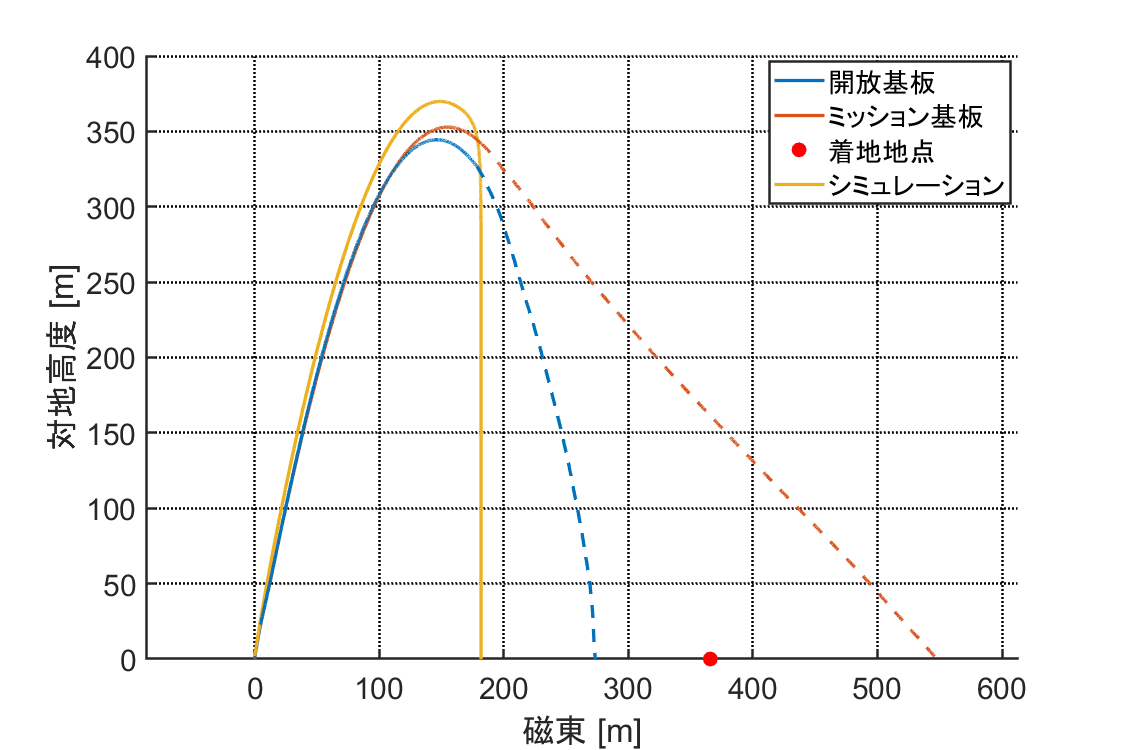
\includegraphics[width=75mm]{pic_sim/pos3_eh.png}
			\hspace{16mm} {\small[1]磁東-対地高度}
		\end{minipage}
		\begin{minipage}{.48\textwidth}
			\centering
			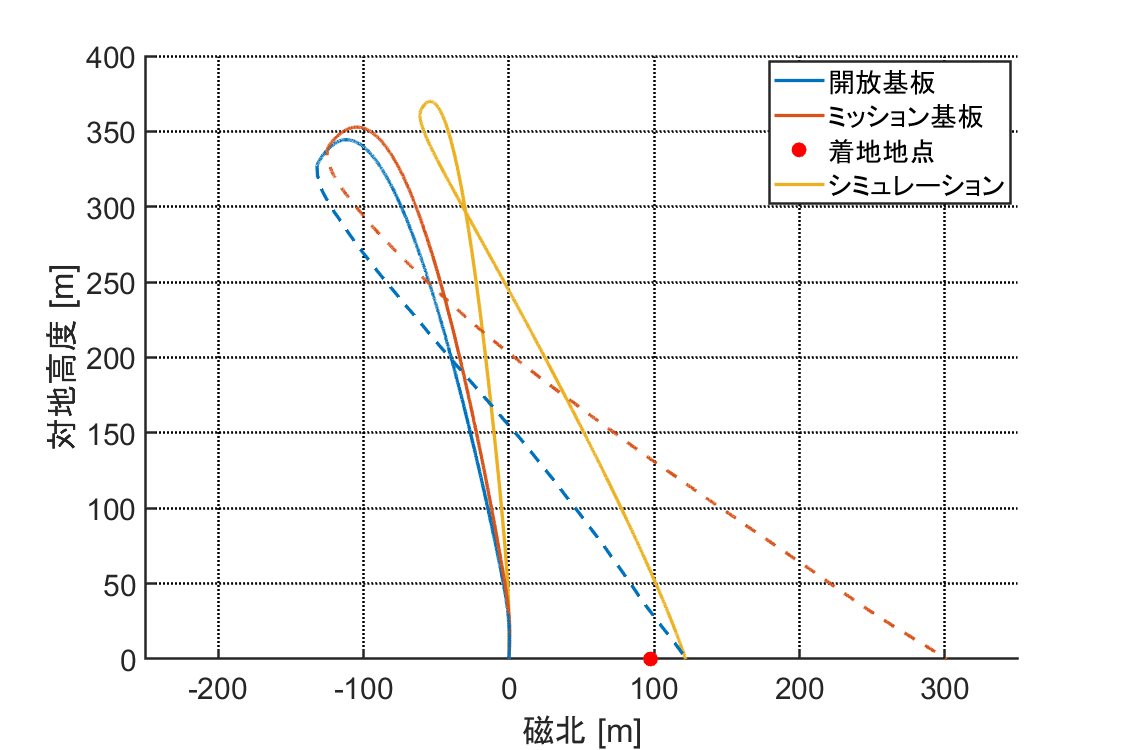
\includegraphics[width=75mm]{pic_sim/pos3_nh.png}
			\hspace{16mm} {\small[2]磁北-対地高度}
		\end{minipage}
	\end{tabular}
	\centering
	\begin{minipage}{.48\textwidth}
		\centering
		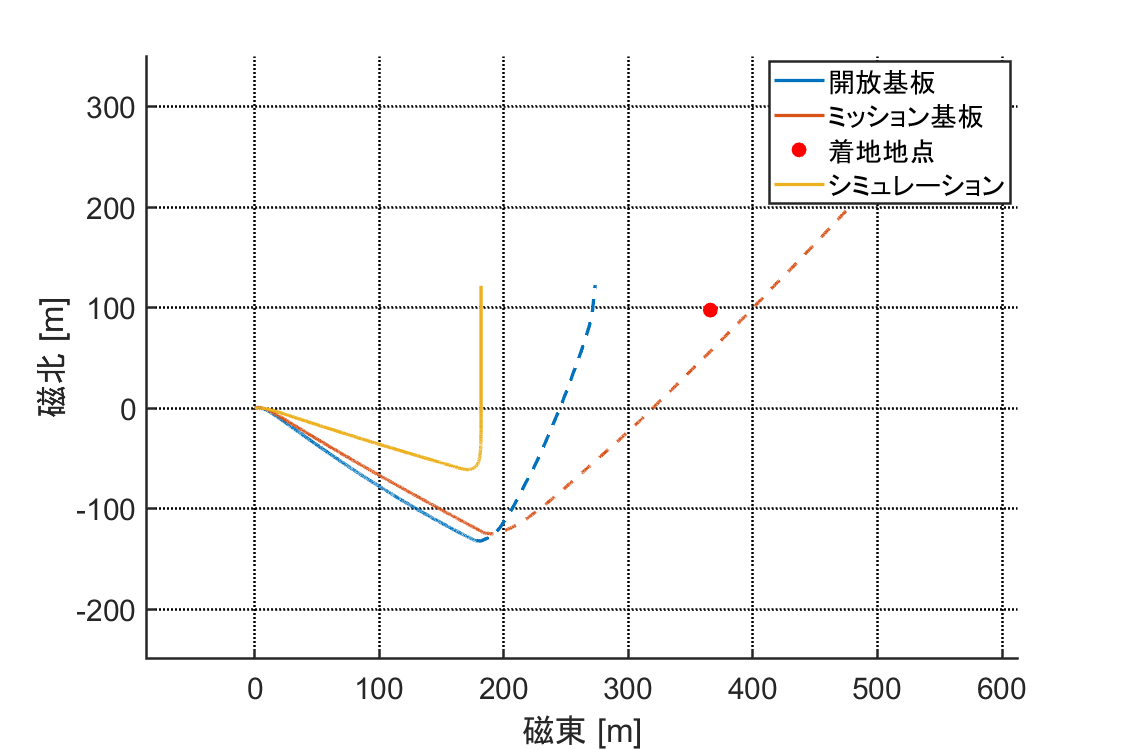
\includegraphics[width=75mm]{pic_sim/pos3_en.png}
		\hspace{16mm}{\small[3]磁東-磁北}
	\end{minipage}
	\caption{飛行経路(風向\SI{180}{deg}風速\SI{3.0}{m/s})}
	\label{fig:hikoukeirosim}
\end{figure}

報告された風向風速条件ではシミュレーションによる落下地点は実際の落下地点から西に約\SI{180}{m}ずれていることが確認できる。
また、最高高度は\ref{koudo}節で示した値より\SI{17}{m}高い結果となった。
これはシミュレーションに使用した推力履歴が7月の燃焼試験でものであり、\ref{suiryokurireki}節で示したように燃焼試験でのトータルインパルスが実際の値より上回っていた事が原因であると考えられる。

さらに、落下地点の差に関しては、風向の違いが大きく関係していると考えられる。
打上げ直前の現地報告では風向が南であったが、推測された飛行経路の開傘地点と実際の落下地点を考慮すると、飛行時の風は南西であったと推測される。
図\ref{fig:hikoukeirosimu225}に南西の風でのシミュレーションの結果示す。

\begin{figure}[H]
	\begin{tabular}{cc}
		\begin{minipage}{.48\textwidth}
			\centering
			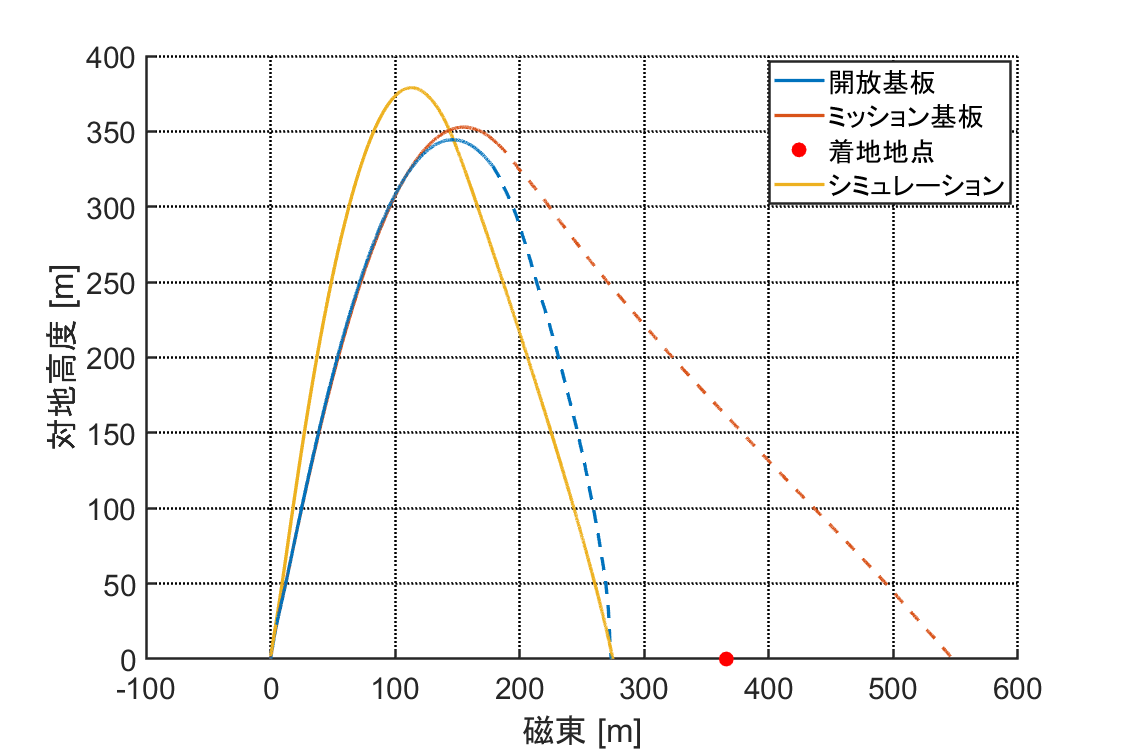
\includegraphics[width=75mm]{pic_sim/pos3_eh_225.png}
			\hspace{16mm} {\small[1]磁東-対地高度}
		\end{minipage}
		\begin{minipage}{.48\textwidth}
			\centering
			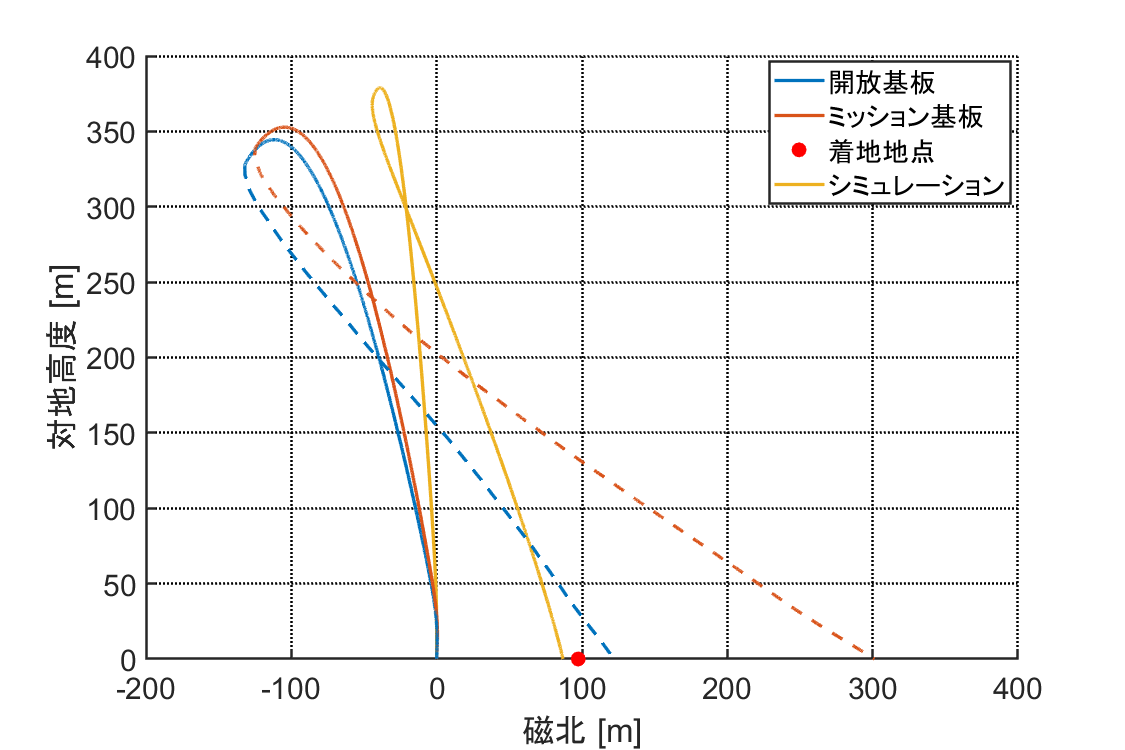
\includegraphics[width=75mm]{pic_sim/pos3_nh_225.png}
			\hspace{16mm} {\small[2]磁北-対地高度}
		\end{minipage}
	\end{tabular}
	\centering
	\begin{minipage}{.48\textwidth}
		\centering
		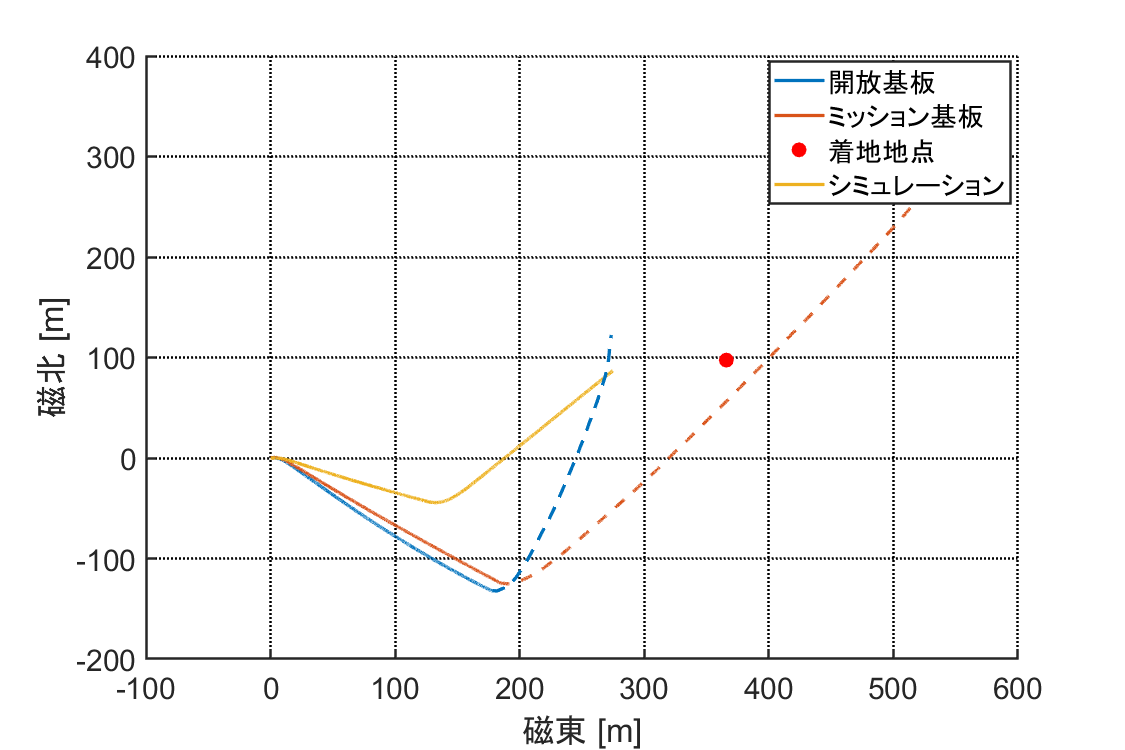
\includegraphics[width=75mm]{pic_sim/pos3_en_225.png}
		\hspace{16mm}{\small[3]磁東-磁北}
	\end{minipage}
	\caption{飛行経路(風向\SI{225}{deg}風速\SI{3.0}{m/s})}
	\label{fig:hikoukeirosimu225}
\end{figure}

結果としては、南の風でのシミュレーションよりも南西の風でのシミュレーションのほうが落下地点に近くなり、実際の落下地点から西に約\SI{80}{m}であった。

\newpage
\section{プロジェクトのまとめ}
\subsection{サクセスクライテリアの達成状況について}
打上結果を基にして、サクセスクライテリアの達成状況を確認する。以下にサクセスクライテリアとその達成状況についてまとめた表を示す。
\begin{table}[H]
	\centering
	\caption{サクセスクライテリアとその達成状況}
	\begin{tabular}{cp{60mm}p{60mm}c} \toprule
		     & \multicolumn{1}{c}{内容}                               & \multicolumn{1}{c}{判定条件}             & 達成状況 \\ \midrule
		MIN  & 地上で制御プログラムを実行し、動翼の適切な動作を確認する。                        & 動画とデータ解析により、意図した動翼の動作が実現していることを確認する。 & 達成   \\ \midrule
		FULL & ロール制御を成功させる。                                         & 搭載カメラの映像とデータ解析によって確認する。              & 達成   \\ \midrule
		ADV  & 制御前に機体がロールをしていた場合、制御中は目標角からのロール角度を\SI{90}{deg}以下にする。 & データ解析で内容を達成しているか確認する。                & 達成   \\
		\bottomrule
	\end{tabular}
	\label{tab:success_criteria_2}
\end{table}
まず、地上試験において動翼の適切な動作の確認は打上前に行った。そのため、MINは達成できている。
また、FULLについては機体搭載のカメラ映像と6軸センサにより、制御中の機体のロール角度が一定に保たれていることが確認されたため、FULLも達成できている。
最後にADVについては、\ref{sc:data_doyoku}節で考察しているように非常に精度の良いロール制御ができており、明らかにクライテリアの内容は達成できている。
以上より、本プロジェクトのサクセスクライテリアはMIN、FULL、ADV全てを達成できたと結論付ける。

\subsection{総括・今後の展望}
本プロジェクトの結果は打上前の期待を大幅に上回るものとなった。搭載していた全センサのデータを完全な形で取得することができ、団体初のロール制御も非常に精度よく行うことができた。
以上の結果を踏まえると、今後は更なる技術発展を目的としたピッチ・ヨー制御に挑戦することも十分に可能である。
また、今回のロール制御は機体のロール角を制御中一定に保つことを目的として行われたが、目標ロール角に収束後、新たな目標ロール角を設定して
その角度へ制御することに挑戦することも面白いと考えている。
また、二段式ロケットであるC-43Jでは機体の姿勢が不安定であったがために二段目の射出を行うことができなかった。
そのため、姿勢制御技術を発展させて二段式ロケットプロジェクトに再挑戦するといった取り組みも行えれば良いと考えている。

\section{謝辞}
本打上実験の実施に際して、多大なご支援をいただいた株式会社天の技様、工機ホールディングス株式会社様、NEWS COMPANY様、ミスミグループ本社様、東京工業大学工学院機械系同窓会 白星会様、
CREATE OB・OGの皆様、顧問の中西先生、運営の皆様、大島町役場の皆様をはじめとする多くの方々に厚く御礼申し上げます。

\begin{thebibliography}{99}
	\bibitem{hikourikigaku} 嶋田有三・佐々修一,飛行力学,森北出版 (2017).
\end{thebibliography}



\end{document}
